% Options for packages loaded elsewhere
\PassOptionsToPackage{unicode}{hyperref}
\PassOptionsToPackage{hyphens}{url}
%
\documentclass[
  12pt, openany]{book}
\usepackage{lmodern}
\usepackage{amssymb,amsmath}
\usepackage{ifxetex,ifluatex}
\ifnum 0\ifxetex 1\fi\ifluatex 1\fi=0 % if pdftex
  \usepackage[T1]{fontenc}
  \usepackage[utf8]{inputenc}
  \usepackage{textcomp} % provide euro and other symbols
\else % if luatex or xetex
  \usepackage{unicode-math}
  \defaultfontfeatures{Scale=MatchLowercase}
  \defaultfontfeatures[\rmfamily]{Ligatures=TeX,Scale=1}
\fi
% Use upquote if available, for straight quotes in verbatim environments
\IfFileExists{upquote.sty}{\usepackage{upquote}}{}
\IfFileExists{microtype.sty}{% use microtype if available
  \usepackage[]{microtype}
  \UseMicrotypeSet[protrusion]{basicmath} % disable protrusion for tt fonts
}{}
\makeatletter
\@ifundefined{KOMAClassName}{% if non-KOMA class
  \IfFileExists{parskip.sty}{%
    \usepackage{parskip}
  }{% else
    \setlength{\parindent}{0pt}
    \setlength{\parskip}{6pt plus 2pt minus 1pt}}
}{% if KOMA class
  \KOMAoptions{parskip=half}}
\makeatother
\usepackage{xcolor}
\IfFileExists{xurl.sty}{\usepackage{xurl}}{} % add URL line breaks if available
\IfFileExists{bookmark.sty}{\usepackage{bookmark}}{\usepackage{hyperref}}
\hypersetup{
  pdftitle={Philosophical Ethics},
  pdfauthor={George W. Matthews},
  hidelinks,
  pdfcreator={LaTeX via pandoc}}
\urlstyle{same} % disable monospaced font for URLs
\usepackage[margin=2.5cm]{geometry}
\usepackage{longtable,booktabs}
% Correct order of tables after \paragraph or \subparagraph
\usepackage{etoolbox}
\makeatletter
\patchcmd\longtable{\par}{\if@noskipsec\mbox{}\fi\par}{}{}
\makeatother
% Allow footnotes in longtable head/foot
\IfFileExists{footnotehyper.sty}{\usepackage{footnotehyper}}{\usepackage{footnote}}
\makesavenoteenv{longtable}
\usepackage{graphicx,grffile}
\makeatletter
\def\maxwidth{\ifdim\Gin@nat@width>\linewidth\linewidth\else\Gin@nat@width\fi}
\def\maxheight{\ifdim\Gin@nat@height>\textheight\textheight\else\Gin@nat@height\fi}
\makeatother
% Scale images if necessary, so that they will not overflow the page
% margins by default, and it is still possible to overwrite the defaults
% using explicit options in \includegraphics[width, height, ...]{}
\setkeys{Gin}{width=\maxwidth,height=\maxheight,keepaspectratio}
% Set default figure placement to htbp
\makeatletter
\def\fps@figure{htbp}
\makeatother
\setlength{\emergencystretch}{3em} % prevent overfull lines
\providecommand{\tightlist}{%
  \setlength{\itemsep}{0pt}\setlength{\parskip}{0pt}}
\setcounter{secnumdepth}{5}
\usepackage[Bjornstrup]{fncychap}
\usepackage{cclicenses}
\usepackage{fancyvrb}
\usepackage{booktabs}
\usepackage{longtable}
\usepackage[bf,singlelinecheck=off]{caption}
\usepackage{etoolbox}
\AtBeginEnvironment{centercap}{\scriptsize}
\BeforeBeginEnvironment{epigraph}{\vspace*{2em}}
\usepackage{tcolorbox}

\newsavebox{\FVerbBox}
\newenvironment{FVerbatim}
 {\VerbatimEnvironment
  \begin{center}
  \setlength{\fboxrule}{0pt}
  \begin{lrbox}{\FVerbBox}
  \begin{BVerbatim}}
 {\end{BVerbatim}
  \end{lrbox}
  \fbox{\usebox{\FVerbBox}}
  \end{center}}

%\setmainfont[UprightFeatures={SmallCapsFont=AlegreyaSC-Regular}]{Alegreya}

\usepackage{framed,color}
\definecolor{shadecolor}{RGB}{248,248,248}

\renewcommand{\textfraction}{0.05}
\renewcommand{\topfraction}{0.8}
\renewcommand{\bottomfraction}{0.8}
\renewcommand{\floatpagefraction}{0.75}

%\renewenvironment{quote}{\begin{VF}}{\end{VF}}
\let\oldhref\href
\renewcommand{\href}[2]{#2\footnote{\url{#1}}}

\ifxetex
  \usepackage{letltxmacro}
  \setlength{\XeTeXLinkMargin}{1pt}
  \LetLtxMacro\SavedIncludeGraphics\includegraphics
  \def\includegraphics#1#{% #1 catches optional stuff (star/opt. arg.)
    \IncludeGraphicsAux{#1}%
  }%
  \newcommand*{\IncludeGraphicsAux}[2]{%
    \XeTeXLinkBox{%
      \SavedIncludeGraphics#1{#2}%
    }%
  }%
\fi%

\makeatletter
\newenvironment{kframe}{%
\medskip{}
\setlength{\fboxsep}{.8em}
 \def\at@end@of@kframe{}%
 \ifinner\ifhmode%
  \def\at@end@of@kframe{\end{minipage}}%
  \begin{minipage}{\columnwidth}%
 \fi\fi%
 \def\FrameCommand##1{\hskip\@totalleftmargin \hskip-\fboxsep
 \colorbox{shadecolor}{##1}\hskip-\fboxsep
     % There is no \\@totalrightmargin, so:
     \hskip-\linewidth \hskip-\@totalleftmargin \hskip\columnwidth}%
 \MakeFramed {\advance\hsize-\width
   \@totalleftmargin\z@ \linewidth\hsize
   \@setminipage}}%
 {\par\unskip\endMakeFramed%
 \at@end@of@kframe}
\makeatother

\makeatletter
\@ifundefined{Shaded}{
}{\renewenvironment{Shaded}{\begin{kframe}}{\end{kframe}}}
\makeatother


\newenvironment{rmdblock}[1]
  {
  \begin{itemize}
  \renewcommand{\labelitemi}{
    \raisebox{-.7\height}[0pt][0pt]{
      {\setkeys{Gin}{width=3em,keepaspectratio}\includegraphics{img/#1}}
    }
  }
  \setlength{\fboxsep}{1em}
  \begin{kframe}
  \item
  }
  {
  \end{kframe}
  \end{itemize}
  }
\newenvironment{note}
  {\begin{rmdblock}{note}}
  {\end{rmdblock}}
\newenvironment{caution}
  {\begin{rmdblock}{caution}}
  {\end{rmdblock}}
\newenvironment{important}
  {\begin{rmdblock}{important}}
  {\end{rmdblock}}
\newenvironment{tip}
  {\begin{rmdblock}{tip}}
  {\end{rmdblock}}
\newenvironment{warning}
  {\begin{rmdblock}{warning}}
  {\end{rmdblock}}
\newenvironment{question}
  {\begin{rmdblock}{question}}
  {\end{rmdblock}}
\newenvironment{slides}
  {\begin{rmdblock}{slides}}
  {\end{rmdblock}}

\newenvironment{epigraph}%
{
\begin{flushright}
\begin{minipage}{30em}
\begin{flushright}
\itshape
}%
{
\end{flushright}
\end{minipage}
\end{flushright}
\vspace{1em}
}

\newtcolorbox{argument}{
  colback=black!5!white,
  colframe=black!30,
  coltext=black,
  text width=12cm,
  boxsep=5pt,
  arc=4pt}

\newtcolorbox{anexample}{
  colback=black!5!white,
  colframe=black!30,
  coltext=black,
  text width=15cm,
  boxsep=5pt,
  arc=4pt}


%\newenvironment{argument}{\par\begin{quote}}{\end{quote}\par}

%\newenvironment{argument}{\par\begin{tcolorbox}}{\end{tcolorbox}\par}

\newenvironment{centerpic}{\begin{center}}{\end{center}}

\newenvironment{centercap}{\begin{center}}{\end{center}}

\newenvironment{embed}{\begin{center}}{\end{center}}

\newenvironment{more}{}

\newenvironment{pullquote}{}

\newenvironment{slideshow}{}

\newenvironment{more-text}{}

\newenvironment{video-caption}{\begin{center}}{\end{center}}

\newenvironment{pull-right}{\begin{raggedleft}}{\end{raggedleft}}

%%%% Suppress title page

\let\oldmaketitle\maketitle
\AtBeginDocument{\let\maketitle\relax}

\title{Philosophical Ethics}
\author{George W. Matthews}
\date{2021-01-28}

\usepackage{amsthm}
\newtheorem{theorem}{Theorem}[chapter]
\newtheorem{lemma}{Lemma}[chapter]
\newtheorem{corollary}{Corollary}[chapter]
\newtheorem{proposition}{Proposition}[chapter]
\newtheorem{conjecture}{Conjecture}[chapter]
\theoremstyle{definition}
\newtheorem{definition}{Definition}[chapter]
\theoremstyle{definition}
\newtheorem{example}{Example}[chapter]
\theoremstyle{definition}
\newtheorem{exercise}{Exercise}[chapter]
\theoremstyle{remark}
\newtheorem*{remark}{Remark}
\newtheorem*{solution}{Solution}
\begin{document}
\maketitle

\thispagestyle{empty}
\begin{center}

{\Huge\textbf{Philosophical Ethics}}



{\Large\textit{a guidebook for beginners}}

\vspace*{2em}


\includegraphics[width=12cm]{img/cover-3.jpg}

\vspace*{2em}

{\large George W. Matthews}

{\normalsize \cc 2020}

\end{center}

{
\setcounter{tocdepth}{1}
\tableofcontents
}
\hypertarget{preface}{%
\chapter*{Preface}\label{preface}}


\hypertarget{dedication}{%
\section*{Dedication}\label{dedication}}


\begin{centerpic}


\includegraphics[width=0.4\textwidth,height=\textheight]{img/hongzhi.jpg}

\end{centerpic}

\begin{epigraph}

Receive correctly this monk's word-stream, neither frozen nor trickling away, neither transparent nor muddy. When you wring it dry, take advantage of the opportunity; when you enter the bustle, perceive with your whole eye. Thorough understanding and the changing world fulfill each other totally without obstacle. The moon accompanies the current, the wind bends the grass\ldots Find your seat, wear your robe, and go forward and see for yourself.\\
~\\
---Hongzhi, \emph{Cultivating the Empty Field}

\end{epigraph}

\hypertarget{about-this-book}{%
\section*{About this book}\label{about-this-book}}


\textbf{\emph{This book}} is an introduction to philosophical ethics intended for use in introductory college or high school level courses. It has grown out of lecture notes I shared with the first students who took my online Ethics course at the Pennsylvania College of Technology almost 20 years ago. Since then it has seen more development in a variety of forms -- starting out as a pdf document, and then evolving into a static set of WordPress pages and finally now as a book written in bookdown and hosted at GitHub. This text represents my attempt to scratch a couple of itches. The first is my wanting a presentation of the major philosophical approaches to ethics that I can actually agree with and that is integrated into my overall teaching method. I tend to teach philosophy to beginners and so there is a fair amount of discussion of the tools used by philosophers and of the ways in which their approach differs from that of their colleagues in other disciplines.

\textbf{\emph{There are}} of course many good quality ethics textbooks out there, and yet none has exactly matched my way of wanting to present the material. Teaching ethics over the years has been a process of active exploration and constant revision of my approach as I have come to a more nuanced and richer appreciation of what ethical thinking and theorizing is all about, as well as some ideas about how I think the main strands of argument relate to each other. Yes this is a partisan effort, but it's all subject to revision and refinement based on, I hope at least, the better argument. That's what I am trying to get across here.

\textbf{\emph{The second itch}} I am trying to scratch has to do with initiatives in open education, and I'd like this text to contribute in its own small way to the much larger and more influential open source movement and philosophy of which I consider it a part. Knowledge is only ours to share. Yes of course writers, developers and publishers do hard work that deserves compensation. But intellectual property, it seems to me, is a false idol that deserves to be smashed. So here is my effort to chip away at it -- knowledge should free us and and not sink us into both literal and figurative debt.

\textbf{\emph{In addition}} the decision to place this text into a \href{https://github.com/gwmatthews/ethics}{GitHub repository} should be considered as an invitation for others to participate in its future development. Anyone can fork the repository where it resides and use it as a template for their own book project; offer suggestions for revisions, or contribute in other ways as well. Please use the ``issues'' section of the repository for making any major suggestions. If you'd like to make your own book from scratch you can read all about how to do it in another book wrtten using the same setup as this one called \href{https://bookdown.org/yihui/bookdown/}{Bookdown: Authoring Books and Technical Documents with R Markdown}.

\hypertarget{acknowledgements}{%
\section*{Acknowledgements}\label{acknowledgements}}


\textbf{\emph{The writing}} and publication of this book would not have been possible without the work of numerous people who make and share their amazing work in the open source software community. It is based in particular on the work of \href{https://github.com/yihui}{Yi Hui Xie} and the other developers of \href{https://bookdown.org/yihui/bookdown/}{bookdown} and \href{https://rstudio.com/products/rstudio/}{Rstudio} and related software. While it has been a bit of a steep learning curve figuring out how to use Rstudio and bookdown to write and style a book, it has been a lot of fun too! The end product, hopefully, speaks for itself and demonstrates that these tools are not just for people with highly technical backgrounds, but can be used by anyone with some computer skills and a bit of patience to create functional, cross-platform and pretty good looking web based books.

Icons are by \href{https://thenounproject.com/ArtZ91/}{Arthur Shlain}.

\hypertarget{license-cc-by-sa-4.0}{%
\subsection*{License CC BY-SA 4.0}\label{license-cc-by-sa-4.0}}


\textbf{\emph{This book}} is released under a creative commons \href{https://creativecommons.org/licenses/by-sa/4.0/}{CC BY-SA 4.0} license. This means that this book can be reused, remixed, retained, revised and redistributed (including commercially) as long as appropriate credit is given to the authors. If you remix, or modify the original version of this open textbook, you must redistribute all versions of this open textbook under the same license.

\hypertarget{how-to-use-this-book}{%
\section*{How to use this book}\label{how-to-use-this-book}}


\hypertarget{read-it}{%
\subsection*{Read it}\label{read-it}}


This should be self-explanatory, but be sure not to miss the icons on the top of the screen which enable you to:

\begin{itemize}
\tightlist
\item
  Open up and close the sidebar with the table of contents in it.
\item
  Search within the text for a keyword.
\item
  Change the color scheme or font to make it easier to read.
\item
  Offer editorial suggestions on GitHub (see below for how this works).
\item
  Download a pdf version of the text for offline reading or printing.
\item
  Find out keyboard short cuts for navigation.
\end{itemize}

Also note the arrows on the side of the screen (or down at the bottom if you are reading on a small screen) that bring you to the next or previous pages.

\hypertarget{comment-on-it}{%
\subsection*{Comment on it}\label{comment-on-it}}


If you are a current student in one of my Ethics classes you'll have to do some commenting. When I used WordPress to host this text that was a built in feature. Here I am relying on a third party commenting add-on to the online version of the book. There are many ways to do this, with Disqus being one of the most popular. But we won't be using it since they track users and push lots of advertising. Instead we'll be using a nice tool called Hypothes.is, which \protect\hyperlink{appendix-1}{you can find out all about here}.

\hypertarget{contribute}{%
\subsection*{Contribute to it}\label{contribute}}


If you find a mistake, don't think it's clear in some part, have an issue with any part of it, want something more added, etc. I encourage you to contribute. You can do this in a few ways.

\begin{itemize}
\tightlist
\item
  If you have a GitHub account, you can leave a comment in the box at the end of each chapter. That creates an ``issue'' which others can read or add to as well.
\item
  You can also contribute more directly as a pull request by clicking on the ``edit'' button on the top menu bar -- this will take you to the GitHub repository where the source material lives. There you can fork the repository, make whatever edits you want and then offer them in the form of a ``pull request.'' Any such requests will be subject to discussion unless they are minor issues like typos. If you really think I get things all wrong here, fork the book and make it your own! All of this assumes that you:

  \begin{itemize}
  \tightlist
  \item
    Know what ``git'' even is.\footnote{If you don't, it is a version control system that enables collaboration and it mostly intended for software development, but it can be used for working together on any kind of project that involves electronic files, from novels to operating systems.}
  \item
    Have an account at \href{https://github.com/}{GitHub} -- which is free. And \href{https://pages.github.com/}{GitHub pages} is a great way to get yourself a free website too!
  \end{itemize}
\item
  Send me an email if you know me in the real world.
\end{itemize}

\hypertarget{part-some-preliminaries}{%
\part{Some Preliminaries}\label{part-some-preliminaries}}

\hypertarget{the-examined-life}{%
\chapter{The Examined Life}\label{the-examined-life}}

\begin{centerpic}

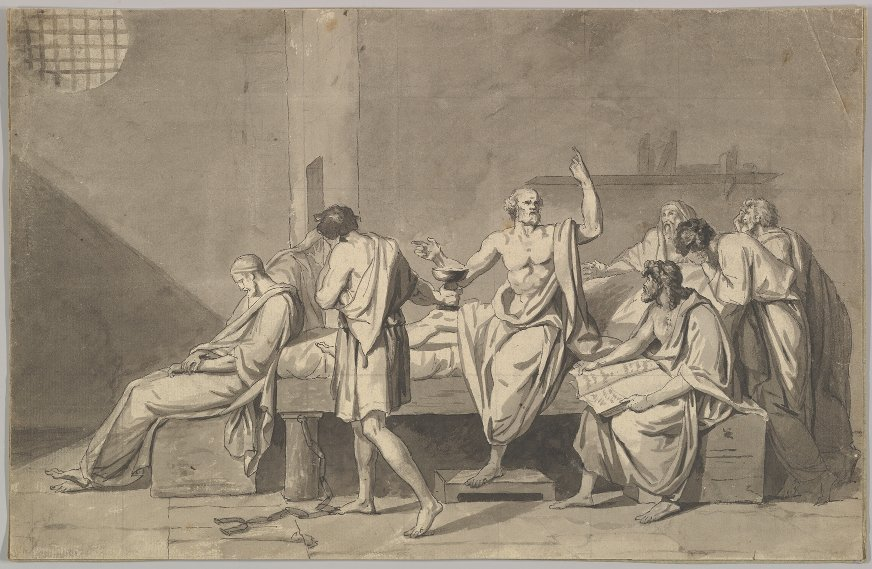
\includegraphics[width=0.5\textwidth,height=\textheight]{img/david-socrates.jpg}

\begin{centercap}

Jacques-Louis David, ``The Death of Socrates''

\end{centercap}

\end{centerpic}

\begin{epigraph}

The unexamined life is not worth living.\\
~\\
---Socrates

\end{epigraph}

\begin{center}

\begin{argument}

Then raising the cup to his lips, quite readily and cheerfully he drank off the poison. Until this point most of us had been able to control our sorrow; but now when we saw him drinking, and saw too that he had finished the draught, we could no longer hold off, and in spite of myself my own tears were flowing fast, so that I covered my face and wept, not for him, but at the thought of my own calamity in having to part from such a friend.\footnote{Plato, ``Phaedo,'' Project Gutenberg, accessed January 12, 2020, \url{https://www.gutenberg.org/files/1658/1658-h/1658-h.htm\#link2H_4_0002}}

\end{argument}

\end{center}

\textbf{\emph{This is Plato's version}} of an eyewitness' account of the last living moments of their teacher Socrates. Socrates was executed in 399 BCE in his hometown of Athens, Greece in the customary way of being given a cup of poison hemlock extract to drink, for the crimes of ``corrupting the youth'' and ``preaching false gods.'' What he really did was spend his days engaging his fellow citizens in dialogue about anything and everything, but especially focused on questions concerning how we all should live our lives, as well as challenging everyone he met to account for and defend their assumptions about how to live. But his relentless questioning earned him many enemies who preferred that the youth, and everybody else, rest content in the assumption that the best way to live is to seek fame and fortune and try to live the ``good life'' that these seem to make possible. Socrates was not convinced and advocated the life of the philosopher, turning away from worldly pursuits and instead reflecting on and critically examining our deepest assumptions and ultimately being willing to admit how little we really know.

\textbf{\emph{Socrates}} was famous for his saying that ``the unexamined life is not worth living.'' What he meant by this is that all of us have a responsibility to examine our own beliefs and try to figure out whether or not they are really true. Not doing this is like sleepwalking through life. This might be pleasant but it runs the risk of us devoting our lives to things that don't truly matter, and even worse it leads us to neglect developing our unique capacity as human beings. Unlike other animals, we can mentally take a step back from what we see in front of us and ask, ``Should I trust what I see or not?'' Likewise with everything we do: we can examine our own desires, intentions and plans and ask ourselves, ``Should I act on these or not?'' In both cases we are capable of distancing ourselves from the immediate demands of our situation and seeking orientation from another source -- we seek \emph{reasons} to believe or doubt what we see and \emph{reasons} to follow or resist our urges. This reflective capacity is the source of our strength since it has enabled us to understand and manipulate the world around us like no other creature on the planet. But, as we can now see more clearly than perhaps Socrates could, it also puts us in the uniquely awkward position of having to justify ourselves to our own worst critics, ourselves.

\textbf{\emph{Another famous, although fictional figure},} who shows the difficulties that our ability to reflect can pose is Shakespeare's Hamlet. Writing at the dawn of the modern era, which saw the expansion of human populations to the current seven and a half billion of us in the span of a few short centuries, and the resulting crowding out of many other life forms, Shakespeare sums up the human predicament when he has Hamlet say,

\begin{quote}
What a piece of work is a man! how noble in reason! how infinite in faculties! in form and moving how express and admirable! in action how like an angel! in apprehension how like a god! the beauty of the world, the paragon of animals! And yet to me what is this quintessence of dust?
\end{quote}

\textbf{\emph{The capacity}} to reflect is the source of both our godlike ``apprehension'' and the difficulties we inevitably encounter in figuring out what we should do with ourselves; our ability to dominate the world we live in and the difficulties we sometimes face in finding a solid sense of purpose and direction. What \emph{should} we really do with our short time here on this planet and why? Should we live our lives according to the standard routine, and accumulate more and more stuff, seeking one ``peak experience'' after another to file away in our memories? Or should we look for a higher purpose, whatever \emph{that} might be? Even though, thankfully, most of us do not experience the tension between these two aspects of our ability to reflect on ourselves and our circumstances quite as dramatically as Hamlet did, all of us face this essentially human predicament -- being masters of the universe and yet feeling lost at the same time. As we will be seeing in this text, philosophical ethics is another, much less bloody, way of exploring it. To set the stage for what we will be up to here I want to first say a bit more about our unique reflective capacity and our ability to pay attention to \emph{reasons}. This was what Socrates had in view when he questioned his fellow Athenians about what they thought was the best way to live. Then I'll turn to a more detailed account of what is distinctive about philosophy in general and philosophical ethics in particular.

\hypertarget{what-do-i-know}{%
\section{What do I know?}\label{what-do-i-know}}

\textbf{\emph{Another Ancient Greek philosopher}}, Plato's student Aristotle, defined human beings as, ``rational animals.'' We are like all other animals and come equipped with nervous systems that enable us to perceive what is happening around us and respond in real time. Animal nervous systems are the product of hundreds of millions of years of evolution, and are extremely useful for helping animals survive and flourish in a complex and constantly changing environment. But what is distinctive about the human nervous system is the degree to which the constant stream of information coming into it through our senses is integrated and organized. It is integrated in an experience which is, as far as we can tell, more fully conscious than that of other creatures. And it can be more explicitly examined and critically reflected on, enabling us to \emph{reason} about how reliable it is and whether what it presents us with is really true. We can make explict to ourselves our own thought processes and subject them to critical analysis.

\textbf{\emph{This is a point}} that it is hard to overemphasize but also easy to miss since we take it so much for granted. By asking ourselves about the reasons we have for believing that some aspect of our experience is true we are asking ourselves not only about the way things seem to us, but about the way things \emph{should} appear; not just what we happen to believe about things based on their appearance to us, but about what we \emph{should} believe about them because it reflects their true reality. And by asking ourselves such questions we are asking what philosophers call \emph{normative questions}, questions that have to do with values, with concepts like right, wrong, good, bad, true, false, beautiful and ugly. We not only perceive and think, but also judge our own perceptions and thoughts according to standards that are more general and weighty, going by the lofty names of Reason, Truth, Reality and so on.

\hypertarget{what-should-i-do}{%
\section{What should I do?}\label{what-should-i-do}}

\textbf{Aristotle also defined human beings} as ``political animals'' since we live together in societies organized around explicit rules and social norms. Here as well we don't have to simply act on whatever urges we feel most strongly, or even just follow along with what others expect of us, we can stop and think about what to do instead and think about whether it is \emph{right} to do or not.

\textbf{\emph{Our ability to reflect}} on our choices and actions introduces a normative dimension to human practical and social life as we come to ask ourselves questions about our own needs, desires and decisions as well as about the rules governing our social lives. We may wonder what we \emph{should do} in some particular situation, maybe when our impulses lead us in one direction and our experience and reason says otherwise; or when we feel social demands imposed on us that we still feel uncomfortable with. Consider the following famous fictional case.

\hypertarget{a-difficult-case}{%
\subsection*{A difficult case}\label{a-difficult-case}}


\begin{question}

Imagine that you are standing next to a railway track and notice a runaway trolley coming down the tracks. There are five children further down the track who are too far away to hear you. There is also a switch in front of you, that would divert the trolley to another track. Unfortunately there is also a single worker on this other track, who is himself to far away to hear you.\\
~\\
\emph{Would you throw the switch and cause the worker to most likely die in order to prevent the runaway trolley from hitting the children?}

\end{question}

\textbf{\emph{This classic case}} of an ethical dilemma has been extensively studied by philosophers and moral psychologists.\footnote{Originally developed by Judith Jarvis Thompson 50 years ago, this problem has lately seen practical application in the development of self-driving cars., Lauren Cassani Davis, ``Would You Pull the Trolley Switch? Does It Matter?'' The Atlantic, 2015, \url{https://www.theatlantic.com/technology/archive/2015/10/trolley-problem-history-psychology-morality-driverless-cars/409732/}} It presents us with a situation in which we most likely feel torn between two alternatives, neither of which seems to be acceptable or desirable, but in which we also may feel unable to refuse to pick either. Cases like this are good at bringing to the surface the intuitions and assumptions we make about what the right thing to do might be, and that is why they are often studied by philosophers and others interested in looking more closely at moral decision making. One significant result of the study of this case is that a large majority of people say that if they were in that situation they \emph{would} throw the switch. Many of us feel compelled to follow a common moral idea: all else being equal, do whatever saves the most lives. But then consider the following variation on this case.

\begin{question}

Imagine that you are standing on a bridge with a low railing over a railway track and notice a runaway trolley coming down the tracks. There are five children further down the track who are too far away to hear you. There is also a very large person standing next to you, and if you gave him a slight push he would fall in front of the trolley car causing it to derail, thus saving the five children.\\
~\\
\emph{Would you push the person off of the bridge in order to prevent the runaway trolley from hitting the children?}

\end{question}

\textbf{\emph{In this case}} a large majority of people say they \emph{would not} push the person off of the bridge even if it would save the five children. Given that the result is the same in either case, the question then becomes why it is that in the this version of this scenario we no longer look at it in terms of gut feeling that it is better to do what leads to more lives being saved.

\textbf{\emph{Whatever the explanation}} for this discrepancy may be (and there is an entire academic industry that has developed around research into the trolley dilemma) the important point here is that philosophers are interested in both examining cases like this directly and in studying how it is that we all tend to respond. Cases like this help us to see and hence to start examining the deeper assumptions we rely on in our thinking about right and wrong. In general this is what philosophy as a discipline is all about -- exposing to view and carefully examining the assumptions we make about how the world works, what we can know about it, and what matters. This is exactly what Socrates meant by leading ``an examined life.'' He insisted that if we never bothered to reflect on our own deepest assumptions about reality, knowledge and values we would be missing out on what may truly make life worth living. You may disagree with him that this kind of examination is something that we should all devote our entire lives to as he did, but he does have a point worth considering. If we never take the time to deeply reflect on our assumptions, are really ever living \emph{our own} lives?

\hypertarget{philosophical-ethics}{%
\section{Philosophical Ethics}\label{philosophical-ethics}}

\textbf{\emph{Philosophical ethics}} is nothing but the deliberate pursuit and clarification of this kind of reflection on our own values, actions and decisions. Even though, as I have been emphasizing, we all have the capacity to reflect on our lives and choices, we do not always spend the time or make the effort to do this carefully and deeply. This is because we are mostly preoccupied with the immediately practical details of our lives. We are too busy living to take the time to stop and think about the significance of what we are doing. However, at times in the lives of both individuals and societies the need to reflect more clearly on what we are doing becomes more urgent. For individuals the need to stop and think and to reconsider the basic assumptions on which we act often arises in relation to important life events or radical changes -- the sudden loss of a loved one; the birth of a child; living through a natural disaster or a war; or even the transition to adulthood in which one assumes full moral and legal responsibility while also gaining the full rights and privileges of adults. These are topics and situations, as we will see later, that are often the focus of discussions in the branch of philosophical ethics called applied ethics. In the case of societies, philosophical thinking likewise flourishes in times of great stress or change -- for example when radically different societies suddenly make contact with each other; when new groups and ways of living displace old groups and ways; when new discoveries challenge peoples' basic views of the nature of things; when societies find their very existence threatened by seemingly insurmountable obstacles. In cases like these it becomes more obviously important to reflect carefully on what we assume is valuable to us both individually and as a society, on what counts as a good life.

\textbf{\emph{A philosophical approach}} to ethics, or moral philosophy\footnote{Throughout this book I'll be using the terms ``ethics'' and ``morality'' as basically synonymous. Some people distinguish between the two terms in one way or another and that is fine as far as it goes. But since the reason English has both terms is that we borrowed each from a different language -- ``ethics'' comes from Greek, while ``morality'' comes from Latin -- and both original terms mean something pretty similar, I see no reason to insist on any fundamental different meaning between them.}, looks at a few different kinds of questions. So the broader field of ethics can be divided up into a few different sub-fields. These are:

\hypertarget{descriptive-ethics}{%
\subsection*{Descriptive ethics}\label{descriptive-ethics}}


\begin{question}

\begin{itemize}
\tightlist
\item
  What do people really think about right and wrong?
\item
  How can we best describe and explain people's moral claims and beliefs?
\end{itemize}

\end{question}

\textbf{\emph{Descriptive ethics}} is not exclusively a philosophical approach to ethics -- sociologists, psychologists, anthropologists and other social scientists are also interested in studying people's ethical, moral and social beliefs. From the perspective of descriptive ethics, our beliefs and principles are things to be studied, categorized, organized and explained. This is what social scientists do for a living.

\hypertarget{meta-ethics}{%
\subsection*{Meta-ethics}\label{meta-ethics}}


\begin{question}

\begin{itemize}
\tightlist
\item
  How does ethical thinking work and how does it compare with other forms of thinking?
\item
  Are ethical claims nothing but \emph{opinions} as opposed to the \emph{factual} claims made scientists?
\end{itemize}

\end{question}

\textbf{\emph{Meta-ethics}} is a higher-order or ``meta-level'' discussion \emph{about} ethical thinking. Here again, philosophers as well as social scientists often ask meta-ethical questions in their attempts to understand what is distinctive about ethical thinking as opposed to other modes of cognition. Looking at ethics from this perspective does not involve taking a stand on particular ethical principles or issues.

\hypertarget{prescriptive-ethics}{%
\subsection*{Prescriptive ethics}\label{prescriptive-ethics}}


\begin{question}

\begin{itemize}
\tightlist
\item
  What is \emph{really} the right thing to do?
\item
  What moral principles are really justified and should be followed?
\end{itemize}

\end{question}

\textbf{\emph{This approach}} to ethics is the uniquely philosophical attempt to find the true basis of ethical thinking. We will be spending a lot of time here examining various attempts to give an account of the basis and justification of ethical thought, belief and action. This way of approaching ethics is not scientific, to the extent that science concerns itself with ``value-neutral'' descriptions and explanations of whatever phenomena it is addressing. That philosophy can succeed in making normative claims while remaining based on objectivity and rationality is up to philosophers to establish.

\hypertarget{applied-ethics}{%
\subsection*{Applied ethics}\label{applied-ethics}}


\begin{question}

\begin{itemize}
\tightlist
\item
  What is the right thing to do in real-world cases of ethical controversy?
\item
  What assumptions and principles lie at the basis of ethical controversies?
\end{itemize}

\end{question}

\textbf{\emph{How does all of this play out}} in real life cases? Under this heading are also to be found discussions of ethical issues associated with some particular area of human life, profession, or subject matter -- hence medical ethics, business ethics, legal ethics, environmental ethics, bioethics and so on are sub-fields within applied ethics.

\textbf{\emph{We should keep in mind}} as we proceed that these various approaches are not always so clearly separate from one another. Our description of what people believe about ethical questions, for example, is clearly often informed by what we think they are justified in believing. Nevertheless we should keep in mind the fact that we can look at ethics from each of these different points of view and recognize that failing to do so may result in unnecessary confusion.

\textbf{\emph{In conclusion}} we might say that philosophical ethics involves deliberately reflecting on our ideas about ethics in general and on specific applications of these ideas to actual cases and controversies. Another term for such deliberate reflection is ``critical thinking.'' This should not be looked at as a primarily negative activity as the word ``critical'' might suggest, but as the positive attempt to arrive at the truth of the matter by thinking carefully about what are often complex and ambiguous ideas and concepts. Even though, as I mentioned at the outset, all of us are equally capable of reflecting critically on our own beliefs, desires, actions and values, it does take some effort and quite a bit of practice to be able to do so effectively. This is because critical thinking is a skill like anything else that we might do with our minds (like solve algebra problems or identify different species of trees) and we shouldn't expect to be experts at it from the start. In the \protect\hyperlink{logic}{next chapter} we will look at and get some practice using one of the most important tools for critical thinking -- the logical analysis of arguments.

\hypertarget{slideshow-summary}{%
\section{Slideshow Summary}\label{slideshow-summary}}

\begin{slideshow}Here is a slideshow summary which can be \href{https://gwmatthews.github.io/ethics-slideshows/01-phl210-slides.html}{viewed online}, \href{https://gwmatthews.github.io/ethics-slideshows/pdf/01-phl210-slides.pdf}{downloaded} or \href{https://gwmatthews.github.io/ethics-slideshows/pdf/01-phl210-handout.pdf}{printed}.

\end{slideshow}

\hypertarget{further-exploration}{%
\section*{Further exploration}\label{further-exploration}}


Michael Sandel is a philosophy professor at Harvard who teaches a very popular course called ``Justice'' that explores material that overlaps with this text. His extensive website \href{http://justiceharvard.org/}{Justice with Michael Sandel} also has videos of his lectures from that course the first of which focuses on the famous runaway trolley example.

\href{https://www.theguardian.com/science/head-quarters/2016/dec/12/the-trolley-problem-would-you-kill-one-person-to-save-many-others}{The Trolley Problem}: an account of some recent rearch on the problem.

\href{https://qz.com/1327804/its-impossible-to-lead-a-totally-ethical-life-but-its-fun-to-try/}{It is impossible to lead a totally ethical life}: Ephrat Livni reflects on ethics and everyday life.

\href{https://press.rebus.community/intro-to-phil-ethics/}{Introduction to Philosophy: Ethics}, ed.~George Matthews. A free textbook, part of a series edited by Christina Hendricks.

\hypertarget{logic}{%
\chapter{A Little Bit of Logic}\label{logic}}

\begin{centerpic}

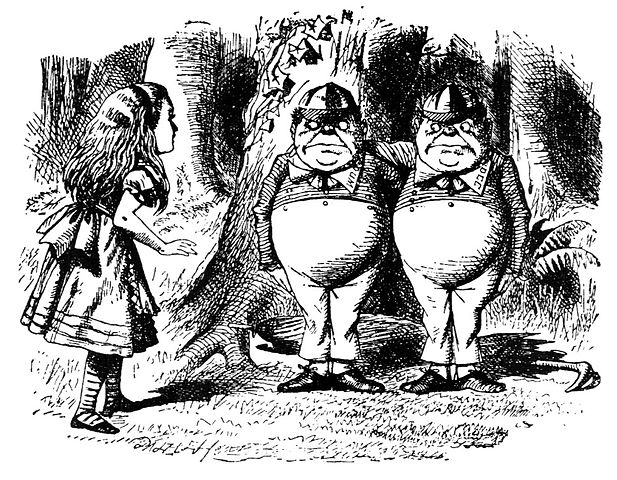
\includegraphics[width=0.5\textwidth,height=\textheight]{img/tenniel-tweedle-dee-dum.jpg}

\begin{centercap}

John Tenniel, ``Alice meets Tweedle Dee and Tweedle Dum''

\end{centercap}

\end{centerpic}

\begin{epigraph}

`Contrariwise,' continued Tweedledee, `if it was so, it might be; and if it were so, it would be; but as it isn't, it ain't. That's logic.'\\
~\\
---Lewis Carroll, Through the Looking Glass

\end{epigraph}

\textbf{\emph{Logic}} is the formal study of reasoning -- the attempt to justify or provide evidence for claims or beliefs. In this chapter we will look at the basic concepts and techniques for the logical analysis of arguments. As we will be seeing this will be useful in our discussions of ethics since much of what we will be doing will involve careful consideration of the justification of claims we make about ethics in general as well as particular topics in ethics.

\textbf{\emph{Before}} we get started though we need to clarify some terminology -- especially our use of the word ``argument.'' Too often this word conjures up a pointless verbal fight between people with opposed views. They argue rather than discuss because their differences of opinion are fixed in place and neither will budge. It is typically a good idea to stay away from arguments in this sense. The word argument as we are using it here, however, has quite a different meaning. For us arguments do not require differences of opinion because arguments are just attempts to explicitly provide back-up or justification for some claim that we might make. We offer arguments in this sense whenever we make the grounds for our belief explicit whether we are doing this within the confines of our own heads, in written form or spoken out loud, and whether or not anyone disagrees with us. Arguments in this sense of the term might appear in regular old verbal disputes. But as we will be seeing, arguments are best looked at one at a time since each one stands or falls on its own merits.

\textbf{\emph{So, for philosophers,}} arguments are just attempts to provide support for whatever it is that we might claim is true. For example, maybe we think the death penalty is wrong, or the opposite, so we come up with an argument to show this. Or maybe we think that morality is a sham, nothing but a cover story for basically selfish motives. Once again, we can come up with an argument in support of this idea. Or on an even more abstract level we might think that moral judgments are just matters of opinion and that it is therefore a waste of time to even argue about what is right and what is wrong. Since none of these claims are self-evidently true (even though some people may think some of these are obvious) we'll need an argument to back them up, or at least to make explicit our reasons for making these claims. In the end, we can think whatever we want. That will, however, only get us so far -- either others will agree with us or not, and either our thoughts will be true or not. But we can also offer reasons in support of our claims in the form of arguments. As we will be seeing, not all arguments are equally persuasive. There are, however, clear-cut and reliable ways of evaluating them to see which really provide the support we are after and which do not.

\hypertarget{arguments-rationality-and-rhetoric}{%
\section{Arguments, Rationality and Rhetoric}\label{arguments-rationality-and-rhetoric}}

\textbf{\emph{Arguments}} can of course be looked at as attempts to persuade other people that they should accept the claims that we are making. Because of this it may seem at first glance to be similar to rhetoric, also known as ``the art of persuasion.'' People who study and practice rhetoric often claim that rational argument is just one among many different methods of persuasion, appropriate at specific times, but not fundamentally different than other methods. That is, they claim that argument is a form of rhetoric. Philosophers, on the other hand, would like to insist on the basic difference between the two. Philosophers call attention to the fact that in rhetoric:

\begin{itemize}
\item
  Appeal is made to our emotions, prejudices, fears, hopes, etc. That is, who we are and what we feel about things matters. This is both its strength and its weakness.
\item
  Because of this, the persuasion that rhetoric produces doesn't last, once our feelings change, we are no longer convinced, and our feelings are constantly changing.
\end{itemize}

In rational argument, on the other hand:

\begin{itemize}
\item
  Appeal is made not to our emotions but to our ability to reason.
\item
  Since everyone is equally capable of reasoning, this means that arguments do not appeal to us personally. It doesn't matter who you are, a good argument should convince you.
\end{itemize}

\hypertarget{the-structure-of-arguments}{%
\section{The Structure of Arguments}\label{the-structure-of-arguments}}

\textbf{\emph{To see}} all of this more clearly, we need to take a look at how arguments work. But first things first -- we need a more precise definition of what we mean by an argument in the first place. That's easy enough:

\begin{note}

An argument is a series of statements where some of these statements are intended to provide evidence or support for others. When we argue we are attempting to establish some claims on the basis of other claims.

\end{note}

\textbf{\emph{As sets of statements}}, arguments involve the declarative use of language. Declarative statements (or propositions) are just sentences that state stuff, they make claims, and so they can be either true or false. So when we are looking at arguments we are deliberately ignoring the many other ways we can use language, such as asking questions, making commands, expressing feelings. When we are offering an argument we are making a series of claims in which some are supposed to provide support for others. The statements that are doing the supporting are known as \emph{premises}. The statement that is being supported, the point of our argument is called the \emph{conclusion}.

\textbf{\emph{It is, however,}} sometimes difficult to tell whether a set of sentences is an argument or not. Let us consider a few examples:

\begin{center}

\begin{argument}

Parents should have the right to make decisions about their own children's healthcare.\\
Why should other people mess around in their business?\\
And please, let's keep the lawyers out!

\end{argument}

\end{center}

This may seem like an argument, so how can we tell for sure? Simply by checking whether this set of sentences is a set of statements where some are intended to provide support for others. So, how many statements are there here? Only one: the first sentence is a statement, the second is a question and the third is a command. In other words, even though this looks at first like an argument it is really just a single claim with no real argument given in support.

\textbf{\emph{What about}} the next example? How many statements are in these sentences? And do any of them really offer support for any of the others?

\begin{center}

\begin{argument}

I am convinced that aliens are living among us and you should be convinced as well.\\
I have really good evidence for this claim.

\end{argument}

\end{center}

Well this is almost an argument, but not quite. There is a claim being made here: aliens are living among us. But there is no real support given for this claim, only the insistence that this person has some unknown evidence. Before we can start to evaluate this evidence to see whether it really supports the claim, we need to see it. So here we have only two separate statements without a real argument yet.

\textbf{\emph{Now consider}} the following example:

\begin{center}

\begin{argument}

Christopher Columbus was a criminal, because anyone who kills innocent people, kidnaps others, and steals their valuables is a criminal and that is just what he did.

\end{argument}

\end{center}

Here the grammatical form is a little misleading. This is an argument in spite of the fact that there is only one sentence. Why? Because this one sentence expresses a few different claims or propositions and some of these claims are offered as supports for others. We can see this if we break it up into individual claims and change the order around like so into \textbf{standard form} with the premises listed as individual statements and the conclusion written last.

\begin{center}

\begin{argument}

Anyone who kills people, kidnaps other people and steals their valuables is a criminal.\\
Christopher Columbus did all of those things.\\

So Christopher Columbus was a criminal.

\end{argument}

\end{center}

Perhaps this is not yet a very convincing or complete argument, but at least it is an argument unlike the first examples.

\textbf{\emph{It is not}} always so clear which statements in an argument are the premises and which statement is the conclusion. Often, but not always, these are signaled with one of a number of typical words or phrases that function as premise or conclusion indicators. Paying attention to these typical words and phrases can help you to disentangle the argument from the peculiarities of a writer's style.

\hypertarget{premises}{%
\subsection*{Premises}\label{premises}}


\textbf{\emph{To help guide}} us through an argument a writer or speaker who is presenting an argument might use the following expressions and phrases to show what the argument rests on. These are \emph{premise indicators}.

\begin{note}

\begin{itemize}
\tightlist
\item
  Because
\item
  Since
\item
  In light of the fact that
\item
  In view of the following evidence
\end{itemize}

\end{note}

This is not an exhaustive list. Basically, when reading an argument you can pick out the premises by asking yourself where the writer is starting from and where he or she is going. The first is the set of premises and the second is the conclusion.

\hypertarget{conclusions}{%
\subsection*{Conclusions}\label{conclusions}}


\textbf{\emph{It is often}} the case that arguments are presented with the conclusion first in order to emphasize where the discussion is supposed to be going. The following common words are often used to indicate a statement that is supposed to play the logical role of the conclusion of an argument.

\begin{note}

\begin{itemize}
\tightlist
\item
  Therefore
\item
  It follows that
\item
  Thus
\item
  It should be clear that
\end{itemize}

\end{note}

These words and phrases indicate that this is where the writer (or speaker) is going with the argument and they are often used at the beginning of an informal argument to orient us, even though logically speaking they are last. For example, when a lawyer begins her argument in court with the claim, ``Your honor, ladies and gentlemen of the jury, my client is not guilty,'' and then goes on to present the evidence, she is reversing the logical order for rhetorical effect. This is fine in everyday life, but since it can be confusing, when we look at arguments explicitly here we will look at them in standard form with the premises first and conclusion last.

\hypertarget{pattern-of-reasoning}{%
\subsection*{Pattern of reasoning}\label{pattern-of-reasoning}}


\textbf{\emph{One other thing}} to watch for when looking at arguments is words and phrases that indicate the structure of the reasoning itself. These are ways of pointing out exactly how the premises are supposed to support the conclusion, and so are indicators of the pattern or form of reasoning involved. Some examples are:

\begin{note}

\begin{itemize}
\tightlist
\item
  Because of these, that has to be true.
\item
  If this then that, otherwise this.
\item
  All of the above is true so this means\ldots{}
\item
  This is the only option that makes sense.
\item
  If we assume that this is true we get a ridiculous result so it can't be true.
\end{itemize}

\end{note}

These indicate the general logic form of argument being followed. Is it a matter of necessity, other conditions present or absent, summation of influences, or a process of elimination, or are we showing something indirectly by showing that denying it makes no sense? The more formal study of logic looks carefully at these and many other different patterns of reasoning, and we will meet them at various points in our discussions of arguments about topics in ethics.

\hypertarget{validity-and-soundness}{%
\section{Validity and Soundness}\label{validity-and-soundness}}

\begin{note}

Being rational is nothing more than trying to follow two basic rules.

\begin{enumerate}
\def\labelenumi{\arabic{enumi}.}
\tightlist
\item
  \textbf{Have good reasons for your fundamental beliefs.} Don't just repeat them because you have heard them, but own them because you have thought them through and they seem to present a defensible picture of how things should be.
\item
  \textbf{Adjust your theories to the evidence.} NOT the other way around! Theories are nothing but models that help us see what might happen next. If our theories keep telling us that something will happen and it doesn't so much the worse for the theory.
\end{enumerate}

Well established theories have both a cogent theoretical story to tell, but also mesh with the facts on the ground. Because of this they can help guide us through our lives. Bad theories that fail either on the theoretical or empirical side, are no better than guesses.

\end{note}

\textbf{\emph{Not all arguments}}, however, are really equal. Just having any old argument won't always get us very far. Instead, as we will see, there are some arguments that really are better than others. This was the insight of the first philosophers in the Western tradition, Socrates, Plato and Aristotle, and it does seem kind of strange that I feel compelled to have to justify it even after a couple of thousand years. Way back then, just like now, many people thought this was a presumptuous claim to make. This is especially the case since it amounts to the claim that some arguments are really compelling on their own, and that we should, as long as we are being rational, have no choice but to accept them. For the skeptics out there who doubt that we will ever be able to create such an argument, I should also point out that the clearest and best arguments really don't end up saying anything very controversial or extraordinary. This is one of the limitations that logic imposes on us: if we are really being logical and using only reliable arguments we may have to refrain from claiming to be able to establish very much. Understanding the logic of arguments, if nothing else, should encourage us to be a little more modest in our claims to knowledge. And this is why Socrates, in spite of his reputation for being a bit of a jerk in pointing out to many people the flaws in their own arguments is today most well known for saying that the only thing he really knew what how little he knew.

\textbf{\emph{To get back to business,}} when we are arguing what we are doing is trying to establish the truth of something that we don't know on the basis of other things that we already know or accept. What we are interested in is establishing the truth of the conclusion, yet for some reason it's truth is not obviously apparent to us so we need to establish it on the basis of other claims the truth of which we can already accept. Arguments move us from the known to the unknown.

\textbf{\emph{To take}} a simple example, suppose we would like to establish that Socrates fears death. We don't have any direct reason for thinking that this is true. But we do know some other things that may be of use in establishing this. First we know that Socrates is a human being. Second we know that all human beings are mortal. Third, we know that all mortals fear death. In standard form this would be arranged like so:

\begin{center}

\begin{argument}

Socrates is a human being.\\
All human beings are mortal.\\
All mortals fear death.\\

So Socrates fears death.

\end{argument}

\end{center}

This is a bit of a contrived example, but it can help us to see the key concepts we can use to evaluate any argument at all.

\hypertarget{key-concepts}{%
\subsection*{Key concepts}\label{key-concepts}}


\textbf{\emph{The information}} in the premises is enough information, as we can easily see, to establish our conclusion. Since Socrates is human he must be mortal, and he must fear death, since all mortals fear death. This argument seems like a pretty solid piece of reasoning. But how can we tell in general whether an argument is a good argument? It turns out that there are two questions we will need to ask about an argument in order to determine whether or not it is a good argument:

\begin{note}

\begin{itemize}
\tightlist
\item
  Is there a clear and solid connection between every step of the reasoning that leads us inevitably from premises to conclusion? In philosophical terminology: \textbf{is it valid}?\\
  ~\\
\item
  Are the claims that we started from, our premises, really true? In philosophical terminology: \textbf{is it sound}?
\end{itemize}

\end{note}

How do we answer these questions for the example above? It seems that there is in fact a clear and solid connection between what the premises are saying and what the conclusion is saying. In fact we already showed this above when showed that the conclusion necessarily follows from the premises. Technically this is a short and informal \emph{proof} of its strength as an argument, that is, of its validity. So the answer to the first question is, yes, it is valid.

\textbf{\emph{As far as}} the second question goes, however, we may have our doubts. Are all of the premises really true? Socrates is (or was) a human being -- he was one of the first philosophers. And all human beings are in fact mortal, at least as far as the evidence we have goes. But do we really know whether all mortals, past, present and future fear death? So here is the one small weakness of the argument. If we could be assured that this premise was true the argument would be completely convincing and would provide adequate backup for the conclusion. But it rests, unfortunately, on a weak premise, so it is not a sound argument. Since these two ideas are both very important for everything we'll be doing here and not so obviously obvious, here are some more explicit definitions:

\begin{tip}

The best arguments must be both \emph{valid} and \emph{sound.}

\begin{itemize}
\item
  \textbf{Validity}: in a valid argument IF the premises are true the conclusion MUST also be true.
\item
  \textbf{Soundness}: A sound argument is a valid argument that also has TRUE premises.
\end{itemize}

\end{tip}

One thing to notice here is that the test for validity is entirely independent of the test for soundness. It is a little misleading, as we can now see, to ask whether arguments are either good or bad. More precisely, they can be:

\begin{itemize}
\item
  \emph{Valid and sound}: these are the best arguments, because the premises really establish the conclusion, and the premises are true -- hence the conclusion really is true.
\item
  \emph{Valid but not sound}: these are promising arguments that exhibit good logical form, but that rely on less than perfect information in their premises, and so are not completely solid.
\item
  \emph{Invalid}: these arguments are bad arguments since they do not establish what they claim to be establishing. All invalid arguments are automatically unsound, since sound arguments are a subset of valid arguments.
\end{itemize}

\hypertarget{more-examples}{%
\subsection*{More examples}\label{more-examples}}


\begin{note}

\emph{Theoretical and Empirical Claims}

Complex arguments about moral issues typically have two primary kinds of support, theoretical claims and empirical claims.

\begin{itemize}
\tightlist
\item
  \textbf{Theoretical Claims} are premises that spell out the bigger picture about how we are looking at things. These can range from explicit statements of methodology and scientific support to implicit ideological frameworks and assumptions.
\item
  \textbf{Empirical Claims} are factual claims on which the application of our theory to reality rests. If our theory says that this economic policy will cause that change in unemployment rates and it consistently doesn't happen that way, we have a flawed theory. So empirical claims are where we provide evidence that shows as much as we can how it is that our theory makes a difference in reality. This is an important part of moral argument as well since it is often the case that our ideas about morality depend on our ideas about what humans really do in certain kinds of cases, so we should at least get that right.
\end{itemize}

\end{note}

\textbf{\emph{Learning how}} to identify valid arguments is important for a course in philosophical ethics, since the philosophical approach to ethics consists largely of the examination of arguments about ethical issues. And the best way to learn this is by practicing. Consider the following argument, conveniently written in standard form:

\begin{center}

\begin{argument}

The earth is a rotating sphere moving around the sun.\\
We are all on the surface of the earth.\\
Anything on the surface of a moving object moves with that object.\\

So we are all moving around the sun.

\end{argument}

\end{center}

Forget for a moment about whether or not you buy the conclusion on its own. In analyzing an argument we need to know whether the premises support the conclusion adequately, so we pretend that we are not sure about the truth of the conclusion. Our first test is the test of validity. We ask ourselves: if the premises were true, could the conclusion be otherwise? Is the truth of the conclusion guaranteed by the truth of the premises? In this case it seems clear that if we are in fact all on the surface of an object that is moving around the sun, then we would all also have to be moving around the sun. So the argument is valid.

\textbf{\emph{Notice}} that establishing an argument's validity is not yet establishing that the conclusion is really true. It is only establishing that the conclusion would be true, if only we could show that the premises were true. In fact this argument was rejected until about 500 years ago because nobody was willing to accept the truth of the first premise. Establishing that this was true took quite a bit of effort by Copernicus, Kepler, Galileo and other early modern scientists. However, we now know that the premises are true. So this argument is not only valid, but also sound. And since it is sound we have proven beyond the shadow of a doubt that the conclusion is true. One more thing to point out here is that this argument has always been sound (or at least as long as the solar system has existed) even if many people denied the truth of the first premise. They were simply mistaken in this denial.

Let's look at another example:

\begin{center}

\begin{argument}

If you want to see the world, you should join the navy.\\
Jane wants to see the world.\\

So Jane should join the navy.

\end{argument}

\end{center}

This argument is a little trickier because it contains an \emph{If \ldots{} then} statement. If \ldots{} then statements, also known as conditionals, make indirect claims. They don't just tell us what is the case, they tell us what would be the case if, or on condition that, something else were true. With this in mind let us consider this second argument. First we check for validity, by assuming that the premises are true and seeing if the conclusion would have to be true as well. In other words we are not yet interested in whether or not they really are true, but whether the argument works as an argument, whether the conclusion logically follows from the premises. It seems pretty clear that this argument is valid. This is because \emph{if}, as the first premise claims, the navy really is the best way to see the world, \emph{and if} as the second premise claims, a person named Jane wants to see the world, then she should clearly join the navy. Notice that this argument's validity does not have anything to do with its content, with the particular claims being made. Instead, validity is a matter of form, so that we could substitute any other content for the content of this argument without affecting its validity. Essentially this argument has the following form:

\begin{center}

\begin{argument}

If A, then B.\\
A.\\

Therefore B.

\end{argument}

\end{center}

\textbf{\emph{Here}} A, B can be substituted by any statements we please, as long as our substitution is consistent throughout the argument. In all cases the resulting argument will turn out to be valid. Try it and you will see that the resulting arguments all come out valid. This is because validity is a matter of logical form regardless of the content we are arguing about.

\textbf{\emph{The soundness}} of arguments, however, unlike validity, has everything to do with content, because an argument is sound when it is valid and it \emph{also has true premises}. Back to the argument about Jane. Is it sound? First we note that it is valid, then we ask whether or not the premises are really true. Consider the first premise: ``If you want to see the world you should join the navy.'' It may be true that joining the navy is one way to see the world (provided that you don't end up on a submarine, or in the engine room of a ship), but is it the only way? Of course not, so the first premise is just false. The second premise is also questionable, but for a different reason -- we simply do not know who Jane is since this is a fictional example. So in spite of its validity this argument is unsound and we need not accept the conclusion as a true statement. It may in fact be true, but this argument gives us no good reason for thinking so. As an exercise you might want to try coming up with a sound argument that follows the form of this one.

\textbf{\emph{Now consider}} as our next example, the following argument:

\begin{center}

\begin{argument}

If you want to see the world, you should join the navy.\\
Jane joined the navy.\\

So Jane wants to see the world.

\end{argument}

\end{center}

This argument seems similar to the previous one, but it has one important difference. The conclusion of this argument was the second premise of the last argument, and the second premise of this argument was its conclusion. What happens to the validity of the argument when we make this simple change? Notice what this argument is saying. It is offering an explanation of why it is that Jane joined the navy -- because she wanted to see the world. The question is, and this is the way we check for validity, are there any other possible explanations of why she joined the navy that are consistent with the premises? In other words, \emph{is it possible for the premises to both be true and the conclusion false}? The answer is yes. It all hinges on what the first premise doesn't say. It doesn't say that the only possible reason to join the navy is the desire to see the world. It just says that if that's what you happen to want then the navy is for you. So Jane could have joined the navy only because she wanted to learn all there is to know about marine diesel engines without caring whether she learned this in New Jersey or in the South Pacific ocean. To put this in yet another way: if it is at all possible, if there are no contradictions involved, for the premises of an argument to be true and the conclusion false, then the argument is invalid. This argument is invalid for precisely this reason. Furthermore, since it is invalid, this automatically makes it unsound, since in order for it to be sound it has to first be valid.

\hypertarget{proofs-and-counterexamples}{%
\section{Proofs and Counterexamples}\label{proofs-and-counterexamples}}

\textbf{\emph{Another}} way to look at the difference between valid and invalid arguments is in terms of the difference between a proof and a counterexample. A proof is a step by step demonstration that the conclusion is a \textbf{necessary} consequence of the premises. To prove that a conclusion validly follows from a set of premises we show in a detailed way how a series of obviously valid steps in reasoning lead us to the conclusion. Take the following argument for example.

\begin{center}

\begin{argument}

Fred is older than Wilma but younger than Betty.\\
Barney is older than Betty.\\

So Barney is older than Fred.

\end{argument}

\end{center}

Remember that a valid argument is one in which \textbf{\emph{if}} the premises are true, the conclusion must also be true. So how would we prove that this is the case? Well we just \emph{assume} that the premises are true and go from there. So here is what a proof might look like:

\begin{tip}

The first premise states that Fred is older than Wilma and he is younger than Betty. Wilma doesn't matter here since she isn't mentioned in the other premise or the conclusion, so let's just note that this premise clearly states that Fred is younger than Betty. Now this would mean that Betty is older than Fred, since ``older'' and ``younger'' are inverses. If I am younger than you then you are older than me no matter who we are since that's what ``younger'' and ``older'' mean. Now since Barney is older than Betty, as the second premise states, he must be older than Fred too, since as we just saw, Betty is older than Fred. This follows from the fact that the relationship ``older than'' is a \textbf{transitive} relationship -- if A is older than B and B is older than C A has to be older than C since that's ``just what''older than" means. So our conclusion that Barney is older than Fred is clearly a \emph{logical consequence} of the premises.

\end{tip}

\textbf{\emph{That's all}} there really is to any proof. We have just unpacked the meaning of what the premises are saying in a way that establishes that they entail the conclusion. We don't, in other words, have to add any new information to what is already stated in the premises in order to get the conclusion. In more complicated cases it can take much more effort to show this but all proofs are nothing but such a process of showing that the conclusion is thus ``contained'' in the premises already, which is of course \emph{why} the truth of the premises would guarantee the truth of the conclusion. In a simple case like this we can almost just see the obviousness of the connection between premises and conclusion, and so it might seem silly to spell things out in this much detail, but in more complicated cases there is more room for error so spelling things out like this is important.

\textbf{\emph{Invalid arguments}} in contrast are arguments where we would need something more than what is contained in the premises to get the conclusion. No matter how we attempt to prove our conclusion we will \emph{always} come to some spot where we cannot get any closer to the conclusion. So how do we show \emph{this}? We use a counterexample, which is nothing but a possible situation in which the premises would all be true and the conclusion would be false. This shows that the argument is invalid, since if it were valid it would be \emph{impossible} for the premises to be true and the conclusion false at the same time as we just saw. Consider the following argument:

\begin{center}

\begin{argument}

Fred is older than Wilma but younger than Betty.\\
Barney is younger than Betty and older than Wilma.\\

So Fred is older than Barney.

\end{argument}

\end{center}

Even though we have no idea what these peoples' ages are (or even if they exist outside of a 1970's TV cartoon series) we can tell that the conclusion does not have to be true, even if the premises were true. This argument is invalid and we can show this with a counterexample.

\begin{longtable}[]{@{}cc@{}}
\toprule
person & age\tabularnewline
\midrule
\endhead
Barney & 36\tabularnewline
Betty & 40\tabularnewline
Fred & 35\tabularnewline
Wilma & 32\tabularnewline
\bottomrule
\end{longtable}

\textbf{\emph{Notice that}} if these people had these ages, this would make all of the premises true and the conclusion false. If Fred is 35, Wilma is 32, Betty is 40 and Barney is 36, then it is true that Fred is older than Wilma, but younger than Betty -- which is what the first premise claims. It is also true that, given these ages, Barney is younger than Betty and older than Wilma -- which is what the second premise claims. But Fred is not older than Barney. In other words, what these ages show that it is \emph{possible} for the premises to be true and for the conclusion to be false and thus that the reasoning involved in getting to the conclusion is invalid. Even if we had true premises, this would not be enough to guarantee the truth of the conclusion. That is what terrible reasoning is all about. We will many more examples of bad reasoning in the next chapter on logical fallacies.

\hypertarget{slideshow-summary-1}{%
\section{Slideshow Summary}\label{slideshow-summary-1}}

\begin{slideshow}Here is a slideshow summary which can be \href{https://gwmatthews.github.io/ethics-slideshows/02-phl210-slides.html}{viewed online}, \href{https://gwmatthews.github.io/ethics-slideshows/pdf/02-phl210-slides.pdf}{downloaded} or \href{https://gwmatthews.github.io/ethics-slideshows/pdf/02-phl210-handout.pdf}{printed}.

\end{slideshow}

\hypertarget{further-exploration-1}{%
\section*{Further exploration}\label{further-exploration-1}}


For a slightly different and more in-depth treatment of the basic concepts of logic see \href{https://jonathanweisberg.org/vip/logic.html\#logic}{the logic chapter} of Jonathan Weisberg's open source textbook on probability and statistics, \emph{Odds \& Ends.}

Wireless Philosophy is a well-produced series of short videos on a great many topics in philosophy. Their \href{https://www.youtube.com/playlist?list=PLtKNX4SfKpzX_bhh4LOEWEGy3pkLmFDmk}{playlist on Logic and Critical Thinking} is a great resource for exploring logical thinking in all of its complexity, 5 or 6 minutes at a time.

\href{https://philosophy.hku.hk/think/}{Critical Thinking Web}: A great site with over 100 free tutorials on many aspects of logic and critical thinking. A nice way to hone your logical thinking skills.

\href{https://www.iep.utm.edu/ded-ind/}{Deductive and Inductive Arguments}: An in depth look at the subject at the Internet Encyclopedia of Philosophy.

\href{https://plato.stanford.edu/entries/abduction/\#}{Abduction}: A close look at the logic of scientific explanation. Gets technical, but the introduction is accessible.

\href{https://youtu.be/4JYL5VUe5NQ}{The Irrationality of Politics}: Michael Huemer is a professor of philosophy at the University of Colorado. This TED Talk by him addresses the question of why we are so irrational when it comes to politics.

\hypertarget{fallacies-and-biases}{%
\chapter{Fallacies and Biases}\label{fallacies-and-biases}}

\begin{centerpic}


\includegraphics[width=0.4\textwidth,height=\textheight]{img/illusion.png}

\begin{centercap}

\href{https://pixabay.com/users/openclipart-vectors-30363/}{OpenClipart-Vectors} at pixabay.com

\end{centercap}

\end{centerpic}

\begin{epigraph}

Reality is, you know, the tip of an iceberg of irrationality that we've managed to drag ourselves up onto for a few panting moments before we slip back into the sea of the unreal.\\
~\\
---Terence McKenna

\end{epigraph}

\textbf{\emph{Throughout}} our discussions of logic so far, you may all have been wondering how often anyone ever lives up to the standards of logical reasoning as we have laid them out here. It may seem fairly obvious that most people do not seem to be either willing or able to accept only those claims that are conclusions of sound arguments, but instead we often decide based on feelings and instincts or on the basis of what we just want or assume to be true at the outset. In fact, there is a theory of the origins of our capacity for logical reasoning known as the ``\href{https://www.edge.org/conversation/hugo_mercier-the-argumentative-theory}{argumentative theory of reasoning}'' that claims that our logical abilities, such as they are, evolved to enable us to ``prove'' ourselves right. Before the abstract study of logic was invented by Aristotle, who sought the universal principles governing reasoning, we were all already adept at persuading others by manipulating logic for the sake of convincing others that we were right and hence asserting social dominance, whether or not our claims were truly justified. It seems, in other words, that the rhetoricians were right after all that logic is just one means of persuasion among others, no better or worse than them, but maybe more or less effective in different contexts.

\textbf{\emph{Or is it?}} As we saw in the last chapter, there is something to be said for being logical. Put simply, valid and sound reasoning really just boils down to not saying more than you really know and this seems like a pretty reasonable approach if we want to figure out what is true and what is not. It is, however, abundantly clear that us humans often fail to abide by this principle and make claims that we really don't have much support for. This chapter explores two related ways we do this -- by committing fallacies and by getting caught by various ``cognitive illusions.'' Fallacies are bad arguments -- they are typically invalid -- that are often used to try to convince someone of some point that really has little argumentative support. They work, to the extent that they do, because they take advantage of certain weaknesses in our reasoning skills. As we will be seeing, a careful analysis of how various different forms of fallacious reasoning work and of what mistakes they make can provide us with a certain degree of protection from those who would use them to convince us of things that have little real support. Cognitive illusions are related in that they lead to mistakes in reasoning, but they are often more difficult to spot and avoid falling prey to, since they are mistakes rooted in mental shortcuts that can be reliable in certain contexts. Like visual illusions, they are false representations of reality, which, even if we know they are false, we cannot help falling prey to. Looking at some common cognitive illusions can help us to see, however, why we should sometimes not trust our own thought processes as much as we often do. And this as well can provide us with more tools for distinguishing between between what is really the case and what just seems to be so.

\textbf{\emph{As we turn to examine}} some important logical fallacies it is helpful to keep in mind that there are both many more particular fallacies than the ones we are going to look at and also many different ways of categorizing them. The thing to keep in mind here is that all stretch logical support beyond its breaking point, and how in particular this happens is not always so clear. On the other hand you can usually see the weakness of an argument that relies on a fallacy by asking yourself a simple question about it: What is being claimed here, and on the basis of what? This often reveals the basic weakness of the argument as it involves stepping back from the particular claims being made in order to see the broader pattern and strategy of reasoning involved. It is this pattern that is flawed, regardless of the content of the argument. As a result, we can often find instances of the same form of fallacious reasoning used with many different topics, especially those that are controversial.

\textbf{\emph{In addition}} it can be helpful to look at fallacies in terms of a few more general types of mistakes in reasoning. That is what we will do here as we examine some different forms of bad reasoning under the headings: \protect\hyperlink{relevance}{fallacies of \emph{relevance}} all of which depend on premises not relevant to the conclusion; \protect\hyperlink{ambiguity}{fallacies of \emph{ambiguity}} all of which depend on the ways in which many words and expressions can have multiple and often incompatible meanings; and \protect\hyperlink{presumption}{fallacies of \emph{presumption}}," which depend on unacknowledged, unjustified extra assumptions.

\hypertarget{relevance}{%
\section{Fallacies of Relevance}\label{relevance}}

\textbf{\emph{As we turn to}} the fallacies of relevance, it is good to remember these fallacies depend on the use of information that may seem relevant to establishing the conclusion but isn't really relevant after all. They often play on our emotional responses to certain situations and topics and they can be quite effective as means of persuading us. They work so well in getting us to buy into their conclusions in part because of the nature of the human mind -- even though we are capable of thinking about things coolly and logically, we often jump to conclusions on emotional grounds and then enlist our cognitive abilities merely to rationalize decisions and conclusions we have already made. Philosophers would encourage us to resist such impulses and to stop and think before jumping to conclusions. This can of course be quite challenging just because of the way in which our brains are wired -- the neural pathway between sensory input to motor and cognitive output is shorter in its trip through those parts of the brain that process emotions than it is through our higher cognitive powers. But still, whoever said leading an examined life was the easiest thing to do?

\hypertarget{appeal-to-authority}{%
\subsection*{Appeal to authority}\label{appeal-to-authority}}


\begin{center}

\begin{argument}

My friend who is a scientist insists that global warming is not cause for alarm, and for me that is a good enough reason to accept her conclusion.

\end{argument}

\end{center}

\textbf{\emph{This fallacy}} is also known as ``appeal to inappropriate authority.'' Appealing to authority is a commonly used way of trying to convince people. But why do we find authorities believable in the first place? Because they are authorities? In this case we may wonder why they are considered authorities at all. On the other hand if they have something to back up their claims, why don't we just see for ourselves whether they are right or not?

\hypertarget{ad-hominem}{%
\subsection*{Ad hominem}\label{ad-hominem}}


\begin{center}

\begin{argument}

There is no need to take that animal rights activist seriously.\\

After all, she also benefits from the use of animals -- notice her leather shoes and fur mittens.

\end{argument}

\end{center}

\textbf{\emph{The name}} of this fallacy is a Latin expression meaning ``against the person.'' It is also known as the ``abusive fallacy,'' or ``personal attack.'' This very popular fallacy focuses on the personal inconsistency of the person giving the argument in an attempt to discredit their argument. People who use this strategy don't respond directly to their opponent's argument but bring up external reasons not to believe anything he or she says. This is clearly wrong since it is the argument that someone gives and its validity and soundness that should be our concern not the person from whose mouth that argument happens to be coming.

\hypertarget{popular-appeal-bandwagon-fallacy}{%
\subsection*{Popular appeal (bandwagon fallacy)}\label{popular-appeal-bandwagon-fallacy}}


\begin{center}

\begin{argument}

The Romans were justified in slaughtering thousands of slaves.\\

After all it was a part of their culture and not many people objected.

\end{argument}

\end{center}

\textbf{\emph{This fallacy}} involves appealing to what most people or the majority of people think as a way of determining what is really true or really right. But as pre-civil rights segregation laws show -- what the majority wants or believes can very easily be wrong. The fallacy known as the ``appeal to tradition'' is similar in that it claims that tradition, the way people have been doing things for a long time, is a good enough basis for us to believe or act as they did. This, of course overlooks the possibility that they were wrong or had no good reason to believe or act as they did.

\hypertarget{appeal-to-force}{%
\subsection*{Appeal to force}\label{appeal-to-force}}


\begin{center}

\begin{argument}

The reason that we are right is because we have the military might to get rid of any government that disagrees.

\end{argument}

\end{center}

\textbf{\emph{However effective}} force or threats of force may be in getting people to do what we want, we may wonder whether this approach really is attempting to convince anyone of anything. Even though threats may get people to say that they agree with you, this shows nothing about whether or not the conclusion is true or whether they really believe what you are saying.

\hypertarget{appeal-to-consequences}{%
\subsection*{Appeal to consequences}\label{appeal-to-consequences}}


\begin{center}

\begin{argument}

If astronomers are correct, the earth orbits a relatively insignificant star in a remote corner of one galaxy among billions.\\

But this conclusion violates our sense of the significance of our own lives and so it must be false.

\end{argument}

\end{center}

\textbf{\emph{This fallacy}} involves rejecting some particular viewpoint, theory or idea based on the consequences to which it leads. These consequences are often emotionally loaded, the kinds of things that we may not want to believe. However, it is often simply irrelevant whether or not we like or want to believe something: the truth may in fact be indifferent to what is pleasing to us. The way to tell what the truth of the matter is, is to examine the evidence rather than reject a theory out of hand because it has unappealing consequences.

\hypertarget{the-naturalistic-fallacy}{%
\subsection*{The naturalistic fallacy}\label{the-naturalistic-fallacy}}


\begin{center}

\begin{argument}

Women alone are capable of having babies.\\

So the responsibility of raising and taking care of them is entirely theirs.

\end{argument}

\end{center}

\textbf{\emph{Next we have}} the naturalistic fallacy. We often appeal to nature as if natural things, practices, etc. were automatically good. This is perhaps understandable in a world filled with various artificial substances of dubious safety. But we should be careful of making such appeals since they involve a leap of logic. The problem with the naturalistic fallacy is actually quite a general problem -- the attempt to conclude something about what should or ought to be be the case from what simply is the case. In this example, the facts of how human reproduction work entail nothing about who should play what role in raising children. That is a matter of social relations that, us philosophers hope, should be based on a free and open (and rational) discussion between those involved and not on the ``facts of life.''

\hypertarget{the-genetic-fallacy}{%
\subsection*{The genetic fallacy}\label{the-genetic-fallacy}}


\begin{center}

\begin{argument}

Newspapers are businesses that make profits from selling papers.\\

So we should distrust what they publish since it is bound to be affected by their desire to make money.

\end{argument}

\end{center}

\textbf{\emph{Arguing like this}} is a more general version of the naturalistic fallacy. We often assume that where something comes from affects its nature in fundamental ways and so we automatically tend to distrust research that is paid for by corporations, we distrust claims made by people who stand to gain from what these claims are about and so on. Although it may seem like wise advice to ``follow the money'' and keep in mind that those who pay the bills might use their power to determine the content of the conversation, insisting that \emph{this must be} the case simply does not follow. In the case of the news media, the fact that a large newspaper corporation makes money for its employees doesn't automatically slant what exactly they are saying in one way or another. This is because one part of their business strategy might also be to maintain high standards of independently verified journalistic integrity. If they are selling their reputation as reliable reporters, and there is an independent way of determining the truth of their claims, there is not necessarily a conflict built into the idea of selling newspapers. Just as in the case of other fallacies of relevance, such as appeal to authority and ad hominem, in this case what matters is not so much who is saying something but what is being said, and we can see for ourselves whether or not it is reliable or slanted in any way.

\hypertarget{red-herring}{%
\subsection*{Red herring}\label{red-herring}}


\begin{center}

\begin{argument}

We shouldn't worry that much about people dying of horrible diseases in Africa.\\

After all we have problems of our own to deal with.

\end{argument}

\end{center}

\textbf{\emph{The name}} of this fallacy comes from the British method of fox hunting. First a captive fox is released and then a pack of foxhounds follow its scent trail, followed in turn by the hunters. In order to make it a little more difficult for the hounds to follow the fox, a piece of smoked herring (a smelly fish that typically is red in color) is wiped on the ground across the fox's path and thrown off to the side somewhere. This serves to distract and confuse the hounds and gives the fox a chance to get away. In an argument whenever you bring up something irrelevant in order to draw attention away from the topic at hand you are relying on the fallacy of red herring. The problem with the reasoning in this example, of course, is that there is no mention made of the possibility that both problems in Africa and problems here can be addressed. Besides mentioning something off the topic in no way undermines whatever claims are made about that topic.

\hypertarget{weak-analogy}{%
\subsection*{Weak analogy}\label{weak-analogy}}


\begin{center}

\begin{argument}

Galileo was ridiculed because of his views, and these views later proved to be correct.\\
I too am ridiculed for believing that the Pope is a reptilian alien in league with the Freemasons.\\

Thus I too will have my day and my views will be accepted.

\end{argument}

\end{center}

\textbf{\emph{Analogies are}} comparisons between different things. We reason analogically when we argue that because one object or concept has a certain feature, other objects or concepts that are similar in certain respects will also have that feature. This is an important way in which we make sense of the world. However, it has its drawbacks. If we are not careful we can end up making analogies when they are not really there. This argument is based on a weak analogy because it is just not the case that all views that are ridiculed end up prevailing in the end. Some do, like Galileo's, but the reason was not inherent in their being ridiculed, but on their being based on good reasoning supported by evidence in the appropriate ways. And by the way, there really are people who believe that the Pope is a reptilian alien, just google it and see.

\hypertarget{ambiguity}{%
\section{Fallacies of Ambiguity}\label{ambiguity}}

\textbf{\emph{The next set}} of fallacies relies on the fact that many terms have multiple meanings. Switching between meanings without acknowledging that one is doing so is a way of making invalid reasoning look valid. Closer examination reveals arguments that do this to be weaker than at first glance. Here we will consider just a few examples. Many more often appear in debates and you can find out about many more examples by following the links at \protect\hyperlink{further-3}{the end of this chapter}.

\hypertarget{equivocation}{%
\subsection*{Equivocation}\label{equivocation}}


\begin{center}

\begin{argument}

People in jail are really free.\\

This is because if you can think whatever you want, then you are free and people jail can certainly think whatever they want.

\end{argument}

\end{center}

\textbf{\emph{Equivocation}} is using multiple meanings of a word as if they were the same. We start out with one meaning of a word like ``freedom'' and end up with another meaning, in the attempt to fool the person who is listening to us that our reasoning is valid. Since many words have multiple meanings it is important to watch out for subtle shifts as an argument progresses.

\hypertarget{straw-person}{%
\subsection*{Straw person}\label{straw-person}}


\begin{center}

\begin{argument}

The senator who suggested cutting funding for the new Air Force attack drone system really wants to leave us defenseless against our enemies.\\

Thus we should reject such cuts.

\end{argument}

\end{center}

\textbf{\emph{This fallacy}} often appears in the context of a debate in which one person misrepresents his or her opponent's view in order more easily to knock it down, like a person made of straw. This is a fallacy of ambiguity in that it relies on a superficially similar version of the view that is being attacked rather than the view itself. One can often ``win'' debates by using this strategy, but such victories are hollow in that they do not really engage with the real issues. If you really want to demonstrate that some view you are attacking is worthy of rejection, it is far better to rely on the ``principle of charity'' and present your opponent's view in as favorable a light as possible. If it still fails, then your position may look even better. The drawback, however, is that if you represent your opponent's views in a more fair and favorable light, your objections to them may themselves not hold up. But that is really only a drawback if you care more about winning debates rather than in figuring things out.

\hypertarget{cherry-picking}{%
\subsection*{Cherry picking}\label{cherry-picking}}


\begin{center}

\begin{argument}

This study of 12 children clearly shows a link between childhood vaccination and autism.\\

Thus vaccines cause autism.

\end{argument}

\end{center}

\textbf{\emph{This one}} is really no joke -- in fact the whole of the current scare about childhood vaccinations and autism was ``established'' by a single study of twelve children! The fact that the paper was retracted, and its author was barred from medical practice didn't matter since its influence only grew since the date of its publication. The logical mistake here is that of selectively reading the evidence in favor of your own hypothesis, or ``cherry picking'' the data to get the juiciest bits while ignoring anything that contradicts it. The other name for this fallacy, ``Texas sharpshooter'' refers to the related practice of proving your worth as a target shooter by first shooting random holes in the side of a barn, and then afterwards drawing your target around a cluster of holes so that it looks like you are a great shot. Is this done in Texas? Probably not, but whoever named it must have had a low opinion of Texans -- no offense intended and if you are from Texas, substitute your state of choice.

\hypertarget{fallacy-of-misplaced-concreteness}{%
\subsection*{Fallacy of misplaced concreteness}\label{fallacy-of-misplaced-concreteness}}


\begin{center}

\begin{argument}

I feel so agitated after I watch the news.

That is not so surprising though, since the media is trying to scare us all.

\end{argument}

\end{center}

\textbf{\emph{How often have you heard someone}} say something like ``it's the media's fault?'' While this may be a common way of talking about things, it makes a subtle mistake in reasoning. It treats an abstract noun, ``the media'' which refers to many different organizations, publications, companies and their vast numbers of employees, owners, stockholders, etc, as if it were a concrete noun: the kind of thing that \textbf{could} meaningfully be referred to as being at fault for something. Concrete things, such as individual people can of course be at fault. Some organizations, such as corporations, can be at fault in a legal sense that they are liable for damages if they do something that is illegal. But can ``the media'' really be at fault for \emph{anything?} What would this even mean? To be at fault for something, I for example, have to knowingly and willingly do something that is illegal or otherwise wrong. But this requires that I can know things and will things, that is, that I am person with a functioning mind.

\textbf{\emph{When we talk about abstractions}} like governments, the media, society and so on, were are no longer talking about particular concrete things, however. Instead we are talking about collections of organizations, institutions, and of course all of the many particular people who run them. And such collections are just not the kinds of things that \emph{can do anything} on their own. This is not to say that individual news agencies, reporters, publishers or whoever, wouldn't be responsible for knowingly publishing false or misleading information. Of course they would be. It is also not to say that there might not be general trends -- clearly governments run by one particular political party tend to do things that governments run by another party would not. It's just that we have to be careful about talking about these abstractions -- the government, the media, society -- as if they were real agents making deliberate decisions. To do so would be to commit the fallacy of misplaced concreteness.

\hypertarget{presumption}{%
\section{Fallacies of Presumption}\label{presumption}}

\textbf{\emph{The third set}} of fallacies we will consider here are those that make presumptions, often in a hidden way. That is, they rely on hidden and unstated assumptions written, as it were, between the lines. This strategy, however, cannot withstand critical analysis since if we can get the perpetrator of such fallacies to acknowledge these hidden presumptions we can see them for what they are, mere assumptions without warrant.

\hypertarget{mere-assertion}{%
\subsection*{Mere assertion}\label{mere-assertion}}


\begin{center}

\begin{argument}

Abortion is just wrong, and that is all there is to it.

\end{argument}

\end{center}

\textbf{\emph{This is}} the simplest and most obvious kind of bad reasoning. As the name implies, mere assertion involves simply stating what you want to establish without presenting any evidence whatsoever to support it. It is truly amazing how often people simply assert something that they may think is true without bothering to offer anything to support this assertion.

\hypertarget{begging-the-question}{%
\subsection*{Begging the question}\label{begging-the-question}}


\begin{center}

\begin{argument}

You should become a Christian.\\
This is because the Bible says that if you are not a Christian you will go to Hell.

\end{argument}

\end{center}

\textbf{\emph{This strange sounding}} name really applies to a very simple technique. Someone who begs the question is guilty of assuming what they are claiming to establish in their argument. In other words they put a disguised version of their conclusion in the premises of their argument. That is, they are not really arguing for what they claim to be arguing for. This is an example of a fallacy that is nevertheless a valid form of reasoning. The problem here is that we cannot just assume that the conclusion is true, as someone who uses this way of argument is in fact doing. Begging the question is not, of course, always so obvious. We can see that this is a case of begging the question when we realize that the only people who will be convinced by this argument are Christians. Why? Simply because nobody else will take evidence from the Bible seriously, and people who consider the Bible as authoritative are already Christians. This example also shows why begging the question is also known as ``preaching to those already converted.''

\hypertarget{appeal-to-ignorance}{%
\subsection*{Appeal to ignorance}\label{appeal-to-ignorance}}


\begin{center}

\begin{argument}

The claim that the death penalty deters crime has not been established with any certainty.\\
Thus it is clear that it does not deter crime.

\end{argument}

\end{center}

\textbf{\emph{The fact that}} something has not yet been proven to be true does not mean that it is false. It is just unknown! Yet this fallacy assumes that if we do not have proof of something then that thing must be false.

\hypertarget{false-dilemma-black-or-white-fallacy}{%
\subsection*{False dilemma (black or white fallacy)}\label{false-dilemma-black-or-white-fallacy}}


\begin{center}

\begin{argument}

Either living organisms are products of blind chance or they were deliberately designed.\\
But it makes no sense that something as functionally complex as a living organism is the result of blind chance.\\

Hence they must have been designed.

\end{argument}

\end{center}

\textbf{\emph{The argument here}} rests entirely on an assumption that is not always so easy to see, the assumption that the alternatives stated are the only ones there are. If this were the case, then the argument would stand, but often other alternatives are simply not even mentioned. Hence the dilemma, or forced choice between two alternatives, is here a false one. In the example below, which is often used against the theory of biological evolution, the missing alternative is precisely what Darwin articulated in his book \emph{On the Origin of Species}, a theory which contains an element of chance but which is not reducible to the blind chance that this argument presumes is the only alternative to deliberate design.

\hypertarget{hasty-generalization}{%
\subsection*{Hasty generalization}\label{hasty-generalization}}


\begin{center}

\begin{argument}

All three of my ex-wives always told me what to do.\\

This clearly shows that all women want to control us men all the time.

\end{argument}

\end{center}

\textbf{\emph{We may be tempted}} to conclude a lot from a single case, or a relatively small sample, but this is often merely a way to confirm our prejudices. If we really want to make sweeping generalizations, we'll have to gather a bit more evidence in less clearly biased ways than this.

\hypertarget{slippery-slope}{%
\subsection*{Slippery slope}\label{slippery-slope}}


\begin{center}

\begin{argument}

If we legalize physician assisted suicide then everyone over sixty had better watch their backs.\\

Once doctors get used to helping people with terminal illnesses die comfortably, they'll find it easier to get rid of older people.

\end{argument}

\end{center}

\textbf{\emph{Slippery slope arguments}} are often used as a way of warning us of the dangers of allowing people to do something that is now forbidden. They say, in effect, if we allow someone to do this, then they'll have no reason not to do that, which is much worse. The name comes from the metaphor of an icy ski slope: if we are foolish enough to step onto the slope, without skis on of course, we'll end up uncontrollably sliding down to the bottom. The problem with this argument is that it claims that we must end up where the arguer claims we will, but the argument gives does nothing but assert that.

\hypertarget{false-cause}{%
\subsection*{False cause}\label{false-cause}}


\begin{center}

\begin{argument}

The majority of heroin users smoked marijuana when they were younger.\\
So smoking marijuana must be one of the causes of heroin use.

\end{argument}

\end{center}

\textbf{\emph{Us humans}} are very good at noticing patterns in the world around us. In fact science is based on this ability -- we notice regularities and then come up with explanations for them. The most powerful of these explanations involve attributing a causal relationship between events that appear to be related to each other in a regular way. We have to be careful here, however, since we also have the tendency to overdo this. This may seem like a convincing argument until we recognize that the fact that something tends to happen before something else is not nearly enough to establish that the first thing causes the second to happen. For example, the fact that my alarm clock goes off every day shortly before sunrise does not mean that my alarm clock causes the sun to rise. The same goes for drug abuse. The fact that I abused marijuana first and then heroin later does not mean that the first caused the second. It is equally possible that I abuse whatever drugs I abuse for another reason -- I have major problems I am trying to escape from.

\hypertarget{circular-reasoning}{%
\subsection*{Circular reasoning}\label{circular-reasoning}}


\begin{center}

\begin{argument}

He must be guilty, since he has a guilty look on his face.\\

Furthermore, the look on his face indicates guilt, because he is the one who did it.

\end{argument}

\end{center}

\textbf{\emph{This final fallacy}} in our list is, in a sense, a more complex version of begging the question. Circular reasoning involves bouncing back and forth between two assumptions each of which is supposed to be the basis for the other. To see the circular structure of the reasoning exhibited here it may help to figure out which statement is the premise and which is the conclusion. In this example, at first glance it seems like the conclusion is ``He is guilty,'' and this seems to be based on the premise that ``He has a guilty look on his face.'' However, the fact that the look on his face indicates guilt is then supported by the assertion that ``He did it.'' Clearly we are moving around in a circle -- our premise supports and is supported by our conclusion. There is thus no real support for either and the whole structure is unfounded. This fallacy is also known as the ``vicious circle'' fallacy.

\hypertarget{cognitive-biases}{%
\section{Cognitive Biases}\label{cognitive-biases}}

\textbf{\emph{Fallacies}}, as we have been seeing, are common mistakes that we make in reasoning especially when we are trying to support a conclusion that we have insufficient evidence to support, ways in which we claim more than we really know. In recent years cognitive psychologists have also explored the ways in which not only get our arguments wrong, but also tend to get things wrong in our own thinking, how as Thomas Gilovich puts it in the title of his book \emph{How We Know What Isn't So}.\footnote{Thomas Gilovich, \emph{How We Know What Isn't So} (New York: The Free Press, 1991)} That is, we have a tendency to fall prey to biases and mistakes in our own reasoning whatever it is that we may end up defending later in our arguments. In this section we'll look at some of the most important and relevant of these cognitive biases.

\textbf{\emph{In general}} we might classify these biases into two general types: ``hot biases,'' or motivated irrationality where our interests, emotional responses or visceral reactions to things influences our thinking process; and ``cold biases'' or unmotivated irrationality which are a result of certain mental shortcuts and routines we rely on even in situations where they do not really apply. Let's look at some examples.

\begin{more}

Hot biases involve bending our reasoning to fit our wants and desires. Because of this definition I believe that hot biases can be pretty easy to spot throughout our daily lives and interactions with others. That is if we take a step back and evaluate our reasoning and emotions within the situation. However, unlike hot biases, cold biases are not results of our desires, but rather they are more like ``bugs'' in our mental operating systems. When you get into cold biases, I believe that this is where things could get tricky.

-- Ryan Moore

\begin{more-text}

The reason I believe that cold biases can be very tricky to spot is that they are simply caused by the way our minds are wired as humans. This means that when dealing with these cold biases in any situation, the odds are already stacked against us. Even when attempting to avoid the use of bias in any situation, debate, or reasoning process, cold biases may rear their ugly heads without us even fully understanding that they are present.

One cold bias strikes me in particular, ``The fundamental attribution error.'' What this refers to is our tendency to be more generous with ourselves when trying to excuse our actions or get ourselves off the hook than we tend to be regarding others. The reason this bias struck me was because, without even noticing it, I have just recently fallen victim to this cold bias in my own life.

To make a long story somewhat short, my girlfriend was in a fender-bender about 2 months back. She was at fault, as she rear-ended the person in front of her. Everybody was okay, and there was minimal damage, but there was still enough damage for it to be noticeable. Well, when I got home from work, she told me the story of what had happened and showed me the damage. In this situation, after she showed me the damage and explained it, I was giving her grief about being more careful when driving probably for the rest of the night. At that point in time, I didn't want to hear any excuses. I was just annoyed that the car was going to need some work. However, not even two weeks after that incident, guess what. I rear-ended someone on my way into work. Honestly though, what are the actual chances? Again, luckily nobody was hurt (besides my ego), and there was very minimal damage. All I had was a cracked headlight and the other car had a small scuff. Well, later that night when I got home from work, I explained to my girlfriend what had happened. However, this time, I was ALL for using every excuse in the book of how it wasn't my fault (when in reality, if you rear-end someone, it's almost always your fault). Looking back on this situation, I fell victim to cold bias. While my girlfriend and I basically committed the same fault, I was much more generous with myself when I was the one who messed up.

Overall, it is my opinion that cold biases can be much more difficult to spot and stop as compared to hot biases.

\end{more-text}

\end{more}

\hypertarget{hot-biases}{%
\subsection*{\texorpdfstring{\textbf{Hot Biases}}{Hot Biases}}\label{hot-biases}}


\textbf{\emph{Hot biases}} are also known as examples of ``motivated irrationality'' because they involve bending our reasoning to suit our wants and desires. Our motivations may not always be clear even to us, so we may not realize that we are caught up in such biases. Luckily, however, there are steps we can take to avoid falling prey to them.

\hypertarget{confirmation-bias}{%
\subsection*{Confirmation bias}\label{confirmation-bias}}


\textbf{\emph{Confirmation bias}} is our often unconscious tendency to give more weight to evidence supporting our pre-existing beliefs or hypotheses and our tendency to downplay the significance of evidence against them. The result is similar to cherry picking but it may not be a deliberate attempt to mislead, but more of a product of other unconscious tendencies.

\begin{center}

\begin{argument}

I keep seeing more and more evidence in favor of my hypothesis! What about the evidence against it? Well that must be based on faulty data collection.

\end{argument}

\end{center}

Given that we have a strong tendency to fall prey to this bias, what steps might we take to avoid it? For one, we can use various ``blind'' methods of data collection and analysis to protect our reasoning from the errors involving confirmation bias. ``Double blind'' medical trials follow these precautions -- to avoid confirmation bias, the patients involved in the trial of a new drug, for example, don't know whether they are getting the drug or a pacebo, and the researchers also don't know whether each particular patient they examine afterwards are in the test group who receive dthe drug of the control group that didn't

\hypertarget{group-think}{%
\subsection*{Group think}\label{group-think}}


\textbf{\emph{Just like}} our pre-existing beliefs can influence what we take the evidence to support, likewise with our connections to other people can do so. When someone in a group we identify with comes up with an idea we have tendency to give it more weight than in fact it deserves. A great example of this occurred during the Kennedy administration with the Bay of Pigs incident. The plan was to send a small group of armed anti-Castro Cuban soldiers to the Bay of Pigs in Cuba with the thought that that would be enough to incite a full-scale revolt against the Communist government by the rest of the Cuban population. Enough members of Kennedy's National Security Council which planned and approved the incursion were strongly in favor of it that they collectively ignored their own military intelligence which indicated that there was little popular support for revolting against the Cuban government. So when the invasion happened in January 1961 the initiative was quickly defeated and the Cuban exiles who landed in the beach were quickly arrested and imprisoned much to the embarrassment of the Kennedy Administration.\footnote{``Bay of Pigs - Groupthink,'' accessed December 2, 2019, \url{https://www.globalsecurity.org/intell/ops/bay-of-pigs-groupthink.htm}}

\hypertarget{wishful-thinking}{%
\subsection*{Wishful thinking}\label{wishful-thinking}}


\textbf{\emph{These last two}} biases could be considered specific examples of a more general tendency we have towards wishful thinking, which is the tendency to project our own desires onto reality and fool ourselves into thinking that reality conforms to how we would like it to be.

\begin{center}

\begin{argument}

I just know that the Yankees will win the World Series, they just can't let me down again!

\end{argument}

\end{center}

All of these biases fail to make a distinction between what we would like to be the case and what really is in fact the case. We may end up lucky and happen to find out that reality conforms to how we would like it to be, but then again we may not. We can protect ourselves against these kinds of biases first by being aware of our own tendencies to fall prey to them and then by using particular strategies to separate our analysis of the evidence from our wishes.

\hypertarget{cold-biases}{%
\subsection*{\texorpdfstring{\textbf{Cold biases}}{Cold biases}}\label{cold-biases}}


\textbf{\emph{Cold biases}} differ from hot biases in that they are not such much results of our desires but of the ways in which our cognitive systems work. They are more like ``bugs'' in our mental operating systems than ways in which we twist our thoughts to conform to our desires.

\hypertarget{anchoringframing-effects}{%
\subsection*{Anchoring/framing effects}\label{anchoringframing-effects}}


\textbf{How much} are you willing to pay for some given product or service? Well it turns out to depend not just on the features of that product or service itself but also by what is next to it on the shelf, what other options you are presented with and even the initial asking price. These are examples of the ways in which the context of our choices influences the content of our choices. Many examples of this can be found in the marketplace. The notorious ``bait and switch'' tactic relies on this bias.

\begin{center}

\begin{argument}

Today only, you can get a new Toyota for 20\% off the sticker price! So act now and drive your new car away today!

\end{argument}

\end{center}

There are numerous ways in which advertisers and salespeople try to influence our choices. First the ``sticker price'' may or may not reflect anything about the reality of the product in question but may be intentionally inflated to anchor our minds to a price higher than we would actually pay. It turns out that doing so will make us more willing to pay a higher price than we would if the original non-discounted price were set closer to what we might actually pay, or what the manufacturer expects us to pay. Likewise, adding extra options that we may not actually be interested in independently can influence our willingness to buy a product, especially when it is compared to an otherwise equivalent product without those potions. In both cases our ability to compare what is offered with what we want is corrupted by the context within which the product is presented.\footnote{For more on anchoring effects see Daniel Kahneman, \emph{Thinking Fast and Slow} (New York: Farrar, Straus and Giroux, 2011)}

\hypertarget{the-fundamental-attribution-error}{%
\subsection*{The fundamental attribution error}\label{the-fundamental-attribution-error}}


\textbf{\emph{When it comes to}} explaining human behavior, and trying to figure out the relative weights of internal factors such as needs, desires and the personality of the actor on the one hand, and external situational factors on the other hand it turns out that we come up with different weights when thinking about our own behavior and that of other people. our own and others. We tend, for example, to put more weight on things outside of our own control when accounting for our bad behavior than we do when accounting for the behavior of others.

\begin{center}

\begin{argument}

The fact that I tripped when walking down the street was because the sidewalk was uneven. When you trip on the other hand, it's evidence that you are a klutz.

\end{argument}

\end{center}

\textbf{\emph{In other words}} we are more generous with ourselves in terms of getting ourselves off the hook --- it's not my fault it's the situation I was in --- than we are with others --- clearly it is their fault! This is true that in many, many cases, if we looked at things in the more neutral terms of finding what factor most influence all of our behavior situational or external factors often play a much greater role than we think. So we are more accurate when we reflect on ourselves than when we look at the behavior of other people. Our attribution of causal influences tends to be skewed in the wrong direction when we look at why others do what they do especially when we compare it with our understanding of what influences us ourselves.

\hypertarget{the-availability-heuristic}{%
\subsection*{The availability heuristic}\label{the-availability-heuristic}}


\textbf{\emph{Finally}} in this brief survey of some major cognitive biases we have the confusion we tend to make between how readily something comes to mind (its ``salience'') and the more objective probability of its occurrence (its ``frequency''). Thus because terrorist attacks are so dramatic and stand out in our minds much more than the more common and mundane threats we are exposed to we tend to be more afraid of terrorism than, for example, driving to the airport. In the aftermath of the 9/11 attacks I remember listening to an interview with an expert on national security threats. The interviewer asked him what we could all do to be safer in international air travel and his response was ``Drive very carefully to the airport.'' This effect, once you start to notice it, is everywhere. We focus on dramatic if also highly unlikely threats and events and ignore those that are far more likely and hence, paradoxically, not so obvious to us.

\textbf{\emph{In this}} and the last chapter we have taken a closer look at what is involved in the justification of any claim at all. We have seen that the best arguments are both valid and sound -- they work logically in that their premises really provide adequate support for their conclusions and their premises are actually true. We have also examined some of the many mistakes in reasoning to which we are prone. These mistakes are not only used in a deliberately misleading way, since all of us have a tendency to make decisions and judgments first and then come up with reasons in support of them later. Thus we often rely on fallacious reasoning to rationalize our own beliefs or we tend to read the evidence is biased ways. As we will be seeing, as we turn now to start examining some of the many different theoretical approaches to ethics, the tools of logic and critical thinking will prove very useful in trying to come up with a reasonable answer to the general question, ``what is the right thing to do?''

\hypertarget{slideshow-summary-2}{%
\section{Slideshow Summary}\label{slideshow-summary-2}}

\begin{slideshow}Here is a slideshow summary which can be \href{https://gwmatthews.github.io/ethics-slideshows/03-phl210-slides.html}{viewed online}, \href{https://gwmatthews.github.io/ethics-slideshows/pdf/03-phl210-slides.pdf}{downloaded} or \href{https://gwmatthews.github.io/ethics-slideshows/pdf/03-phl210-handout.pdf}{printed}.

\end{slideshow}

\hypertarget{further-3}{%
\section*{Further exploration}\label{further-3}}


\textbf{\emph{There are many}} great websites that list, discuss and explain the many ways we get things wrong in our thinking. Here are a few of my favorites.

\href{https://yourlogicalfallacyis.com/}{\emph{Your Fallacy Is}} is a nicely designed website with more examples of common fallacies.

\href{https://yourbias.is/}{\emph{Your Bias Is}} is the sister site to Your Fallacy Is and focuses on common cognitive biases.

\href{https://www.logicallyfallacious.com/tools/lp/Bo/LogicalFallacies}{\emph{Logically Fallacious}} is a site with a huge and comprehensive list of logical fallacies and cognitive biases. A great reference with lots of examples.

And you should of course follow the \href{https://twitter.com/fallacy_ref}{Logical Fallacy Ref} on Twitter.

\hypertarget{part-ethics-culture-and-religion}{%
\part{Ethics Culture and Religion}\label{part-ethics-culture-and-religion}}

\hypertarget{relativism}{%
\chapter{Relativism}\label{relativism}}

\begin{centerpic}

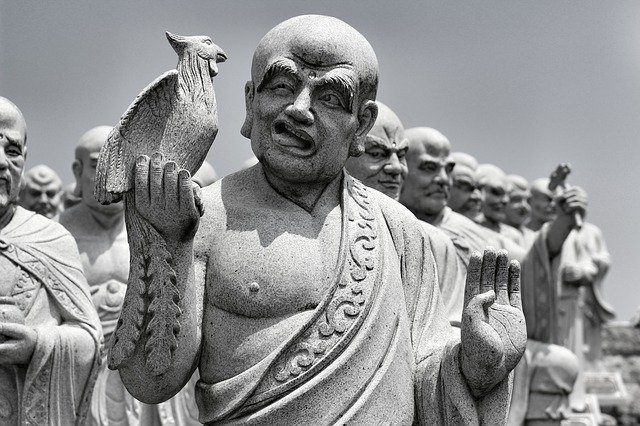
\includegraphics[width=0.5\textwidth,height=\textheight]{img/buddha-bird.jpg}

\begin{centercap}

\href{https://pixabay.com/users/mikhsan-4911734/}{mikhsan} at pixabay.com

\end{centercap}

\end{centerpic}

\textbf{\emph{As we now turn}} to look more carefully at ethics it may help to have a sense of the general approach we will be following here. We'll be looking at a variety of theoretical perspectives on ethics -- perspectives which determine the position one might take regarding questions such as:

\begin{itemize}
\tightlist
\item
  Is ethics just a matter of opinion, or is can ethical principles lay claim to a more universal validity?
\item
  What is the relation between ethics, law and religion -- all of these spell out rules for behavior but on the basis of what and what happens when they come into conflict?
\item
  Is it rational to be ethical or does ethics depend on something other than our ability to think things through?
\item
  Is there anything that is just plain wrong, no matter what the consequences?
\end{itemize}

\textbf{\emph{There are many possible ways}} to consider these questions. I'll be following a fairly common approach that looks at them in the light of various general theories or philosophical positions one might adopt. Each of these theories makes a particular claim about what is fundamental to ethics, highlights certain aspects of our ethical lives and also provides some guidance for dealing with ethical controversies in the real world. These theories have all found both defenders and critics in the history of philosophy although here I will be more concerned with them as general approaches to ethics than with worrying too much about accurately presenting the views of historical thinkers. These theories as I am presenting them can best be looked at as ``ideal types'' that have their own inner logic, and their own strengths and weaknesses as attempts to articulate and defend some version of what ethics is really all about.

\textbf{\emph{In my view}} not all of these theories are equally viable. In fact it seems to me that most of them simply fail as approaches to ethics for a variety of reasons that will become clearer in each case. This brings up the obvious question of why we should bother looking at a whole slew of approaches to ethics that ultimately don't work instead of just more directly articulating one that does. There are two reasons to take this approach. First, in spite of the difficulties faced by these approaches to ethics, \emph{all} of them continue to be popular and find defenders both historically and at the present. Even if these defenses are inadequate, they still have and have had their champions. There is a version of an old joke about anarchists that applies here to philosophers: given three philosophers in a room together there will be four positions taken by them on any topic that comes up for discussion. This is a feature and not a bug of philosophy, since philosophy is the attempt to articulate and defend a general account of such abstract topics as the nature of reality, knowledge and values, so the more particular positions we can examine the better. Just like in science we should welcome a diversity of approaches rather than rule any out at the start. But unlike in science, unworkable philosophical theories have a longer shelf life since the cost for holding on to them is relatively easy to bear. If a scientific theory is fatally flawed that is typically clear -- one's prediction of what the experiments or data will show fails, other explanations cover more cases with fewer assumptions and better fit with the data, the bridge built on the basis of one's calculations collapses. The cost of bad science is steep. In philosophy, however, the costs of holding onto unsuccessful theories is having to put up with theoretical incoherence, to be willing to hold conflicting views in the mind at the same time. And it turns out that us humans are pretty good at doing these things -- all you have to do to live with a poorly worked out set of fundamental beliefs is stop thinking about them.

\textbf{\emph{The second reason}} for considering a multitude of unsuccessful approaches to ethics here is that each of these approaches does have the advantage of focusing on some important aspect of ethics. To the extent that these theories fail it is because they tend to overemphasize the aspect in question and ignore others. Looking at a variety of approaches can thus help give us a clearer picture of what ethics as a whole is all about, even in the absence of some final master theory that would unify ethics once and for all and win universal assent. It seems to me that there is a certain ``logic'' to the story I'll be telling here, even if it is nothing like a necessary development, a magical dialectical unfolding of the Truth about ethics, but I do present each theory as an effort to take in to account the failings of the proceeding accounts. Making sense of our ethical lives and thinking clearly about ethics is hard, but it seems to me that it is worth the effort. Philosophical ethics may not be an empirical science, and debates in ethics may not ever be resolved, but it is a rich field well worth exploring. My presentation here is intended in the spirit of a guidebook, pointing out certain general features of the landscape, some important landmarks and major hazards to be reckoned with.

\textbf{\emph{So much for}} a general account of what we will be up to here. This section of the text looks at two approaches to ethics that may seem to be diametrically opposed -- cultural relativism and the attempt to show how ethics can and should be based on religion. According to cultural relativism, ethical rules and norms are determined by culture in the sense that there are no absolute and universal rules with an independent warrant, but only particular, culturally determined ways of conducting oneself, none fundamentally better or worse than the others. According to religious approaches to ethics, ethical rules and principles do have an absolute foundation and that foundation is to be found is an authoritative set of religious truths. In spite of their obvious opposition, with relativism denying the existence of ethical absolutes and religious approaches affirming it, in a sense both have something essential in common, which is the idea that ethical rules come to us ``from outside'' and have little to do with human choices. Their opposition lies in whether or not the source of ethical rules varies from place to place or not. Both of these approaches will be found wanting, for roughly parallel reasons. And so the next part of the text, which examines various more purely philosophical approaches to ethics, takes up the question of what ethics might look like if it is something we humans create and not imposed from outside by culture, God or human nature.

\begin{note}

\textbf{A note on method:}

In this text I'll be exploring various approaches to ethics chiefly as I understand them. Although at times I make reference to historical philosophers and sometimes to their particular arguments and texts, this book is not intended as a contribution to historical scholarship. Instead my approach is to consider ethics in terms of a series of ``ideal types'' which, while they may overlap with the ideas of certain historical figures, are intended to capture what I understand to be the major lines of argument available to anyone who attempts to clarify basic notions of ethics. There is a certain inner logic it seems to me to how we can, and maybe even should, think about ethics. Or maybe that is just a result of my having spent too much time reading Hegel in my youth. In either case, \emph{caveat lector} -- let the reader beware.

Over time I will also try to expand on and/or make room for approaches I haven't yet had time to integrate into my overall scheme, such as virtue ethics, Buddhist ethics (and non-Western approaches more broadly) and feminist approaches to ethics. \protect\hyperlink{contribute}{I do welcome suggestions} about how to extend and revise this text to make it more inclusive.

\end{note}

\hypertarget{claims-and-consequences-of-moral-relativism}{%
\section{Claims and Consequences of Moral Relativism}\label{claims-and-consequences-of-moral-relativism}}

\begin{epigraph}

If anyone, no matter who, were given the opportunity of choosing from amongst all the nations in the world the set of beliefs which he thought best, he would inevitably -- after careful considerations of their relative merits -- choose that of his own country. Everyone without exception believes his own native customs, and the religion he was brought up in, to be the best.\\
~\\
---Herodotus, The Histories

\end{epigraph}

\textbf{\emph{Opinion}} -- this seems to be where ethics starts and in many people's minds where it ends. You have a right to your opinion about right and wrong and I have a right to mine, so let's just leave it at that. Given what we have been looking at so far, not to mention all of the unread pages still ahead, it is probably already apparent that that is not going to be the whole story about ethics. It is nevertheless a deeply rooted assumption that ethical claims \emph{must be} opinions, since they are clearly \textbf{not} factual claims and that seems to be the only other sort of claim we can possibly be making when we are using language to state things. That this assumption does not in fact hold up to closer inspection is what this chapter is going to argue.

\textbf{\emph{Humans are}} incredibly diverse and in many ways. We are diverse in appearance; we live in many ways in many different environments; we speak many different languages and embrace many different beliefs, practices and norms. People live in almost any conceivable physical environment, from dense tropical jungles, to frozen polar deserts, from small villages with thatched huts to modern industrial cities made of concrete, steel and glass. In addition, our cultural practices and norms reveal perhaps an even greater diversity. Some human cultures place value on devotion to the group at the expense of individual liberty, others emphasize the unique individual while downplaying our relation with others. Some cultures value continuity and tradition while others value innovation and rapid change. Some cultures value constant productive work while others place far more emphasis on living well and enjoying social interaction with others. Some cultures allow men and women to participate equally in all areas of social life, while others have entirely separate spheres for the two sexes. Recognition of this diversity is what has led some philosophers and social scientists to formulate a theory known as ``cultural relativism,'' which takes these casual observations and turns them into an explicit set of claims about the nature of value judgments. This theory is not only a popular theory about the nature of values. It also presents a challenge to the whole enterprise of philosophical ethics since it leads to the view that rational discussion and argument have little role to play in ethical decision making. Ethical decisions, opinions and judgments, according to cultural relativism, are always relative to the cultural environment within which they are made.

\textbf{\emph{Cultural relativism}} is one particular variant of a broader position that holds that moral universals are impossible in principle and that moral judgments are closer to judgments of taste than they are to anything else. Just as with judgments of taste, according to this view, sometimes called ``moral anti-realism'' for its denial that there is any basis in reality for determining what is right and what is wrong, there is little point in arguing about moral issues since they reduce to personal preferences. I won't go into the various versions of this idea here but will focus on the claim that moral values and judgments are essentially rooted in culture. The issues that this view raises, it seems to me at least are broadly the same as those faced by other variants and so dealing with cultural relativism will be enough for our purposes here.

So let us then look more carefully at what cultural relativism claims. It is a \protect\hyperlink{meta-ethics}{meta-ethical} position that boils down to a few simple and seemingly obvious claims:

\begin{note}

\textbf{According to cultural relativism}

\begin{itemize}
\tightlist
\item
  Ethical or moral claims are not objective in the way factual claims are.
\item
  There is no neutral standard for determining right or wrong.
\item
  All value judgments are relative to our personal or cultural perspective.
\end{itemize}

\end{note}

\hypertarget{a-first-case-for-relativism}{%
\subsection*{A first case for relativism}\label{a-first-case-for-relativism}}


\textbf{\emph{At first}} this set of claims may seem obviously true. After all, given the diversity of human values and customs, how could there be anything more than relative standards, standards that are only applicable within a given culture? Many people find relativism intuitively appealing and might even offer as a preliminary case for relativism the following points:

\begin{itemize}
\tightlist
\item
  \emph{Cultural diversity}: Human culture has always been extremely diverse. And many people seem to have equally diverse views on what sort of behavior is acceptable. It seems to follow from this that there cannot possibly be any standards for deciding between these views.
\item
  \emph{How we learn about values}: It seems obvious that we learn about values, and come to accept the values that we do because these are the values that are shared by the people who raise us. They are the values of our families and communities.
\item
  \emph{Intolerance}: There have been plenty of cases throughout history in which one group of people firmly believed that their values were not just acceptable for them but absolutely right, and used this as a justification for committing atrocities against other people. Relativists insist that the only way to avoid this kind of intolerance is to accept that there are no ultimate standards.
\end{itemize}

\hypertarget{what-is-at-stake}{%
\subsection*{What is at stake}\label{what-is-at-stake}}


\textbf{\emph{In a moment}} we will consider each of these points in greater detail. Before we do this it will be helpful to spell out what is at stake here. That is, we should consider what would be the case about ethical principles and decision making if cultural relativism were true. Its defenders make much of the positive consequences of this theory, while its opponents emphasize its negative implications. As we consider these consequences of the theory we must remember that whether or not we like where a theory leads us, in terms of its theoretical consequences, cannot itself determine whether the theory itself is correct. Reality does not care whether or not we like it. In the case of relativism at least, the extreme nature of its consequences helps explain why it is such a controversial theory.

\textbf{\emph{Defenders of relativism}} present it as the best way to acknowledge the great variety of human value systems and cultures. If there are no ultimately correct moral principles, then all human cultures become equally valid as ways of life, at least for different groups of people. This seems to encourage tolerance of other ways, a welcome relief after millennia of people intolerantly fighting with each other over their different views. After all, if there are no ultimate standards for right and wrong, we would could never justifiably say, ``Your group is wrong in doing what you do and so we have the right to force you to change your ways.'' On the other hand, a relativist cannot really consistently promote tolerance -- otherwise she would be granting tolerance for other cultural practices the status of a universal value, valid for everyone and this is what relativism says does not exist. So we should really say that relativism really only rules out one possible way of dealing with conflicts: the rational settlement of differences with reference to some kind of universal principles or values. Sometimes differences of opinions might be tolerated by the members of the groups that differ, sometimes one group will attempt to push its values on the other group. Both approaches are consistent with the claims of relativism.

\textbf{\emph{The first}} troubling consequence of relativism is one you may already have suspected: if there are no real standards, standards about right and wrong that are independent of cultural perspectives, it doesn't seem possible to condemn other cultures or individuals for doing awful things. For example, imagine that there is a society that has two major groups of people. One of these groups, who happen to be the majority of the population, decides that the other group doesn't deserve any respect, perhaps even that they are somehow naturally deficient or inferior. As a result they perform painful and often fatal experiments on the minority group, force them to work without pay, and even decide just to kill them off because it makes them feel better about themselves. What would a relativist say about this? It seems that since the relativist is only willing to recognize local or relative standards, she would have to conclude that although she doesn't like it, or that such behavior would never be tolerated in her society, she really can't condemn what this group of people are doing as simply being wrong. Why not? Well, because it seems right to the majority of people in that other society.

\textbf{\emph{Furthermore}}, relativism, if it were true, would require us to reject the idea that we can really make moral progress. Consider voting rights for women and African-Americans. In early American history both groups were denied these rights. Later on, after the Civil war in the case of African-American men and then in the early twentieth century in the case of all women, the Constitution was amended when people recognized that it was wrong to restrict these groups' access to the political process just because of race or gender. Many of us would consider this a case of moral progress -- a basic right was extended to people who had previously, for no good reason, been denied this right. What would a relativist say? Could they say that this was really a case of progress? Probably not, since progress implies that things are getting better, and this requires that there is some standard against which we can measure better or worse. So, for the relativist there is no such thing as progress, only different ways of doing things, none of which are really better or worse than any others. Is this a conclusion you are comfortable with?

\textbf{\emph{Relativism seems}} like a plausible theory about the nature of value judgments. It also seems, at first glance at least, to be a theory with nothing but positive implications -- it seems to encourage of diversity and lets everyone do their own thing. However, as we have just seen this easy-going character of relativism soon reveals a darker side. A relativist cannot really have any grounds for condemning any behavior at all, no matter how intuitively awful it seems, as long as someone believes that it is OK. In addition relativism does away with one of the most important parts of our moral thinking, the idea that maybe through our efforts we can make things a little better. This idea of progress is rendered simply meaningless by relativism. These implications of relativism do not by themselves let us know whether or not relativism is true. At best they reveal what the stakes are -- if relativism is true we get tolerance at the expense of having to tolerate anything all at that someone feels is the right thing to do. To determine whether or not relativism is true we need to consider more explicitly the arguments in support of this theory.

\begin{caution}

\textbf{Consequences of relativism}

If relativism is true:

\begin{itemize}
\tightlist
\item
  Nothing can be condemned as just plain wrong.
\item
  Moral progress is a meaningless idea.
\item
  Different cultures speak different, mutually incomprehensible moral languages.
\end{itemize}

But remember -- just because a theory has consequences we don't like doesn't mean it's false. Saying so would be a \protect\hyperlink{appeal-to-consequences}{fallacy}.

\end{caution}

\hypertarget{defending-relativism}{%
\section{Defending Relativism}\label{defending-relativism}}

\begin{epigraph}

The life history of the individual is first and foremost an accommodation to the patterns and standards traditionally handed in his community. From the moment of his birth the customs into which he is born shape his experience and behavior.

---Ruth Benedict, Patterns of Culture\footnote{Ruth Benedict, \emph{Patterns of Culture} (Boston and New York: Houghton Mifflin, 1935)}

\end{epigraph}

\textbf{\emph{Thus far}} we have been looking at the pros and cons of accepting relativism as an approach to ethics. In doing so we have been avoiding asking a simple question, that we now cannot any longer avoid -- \emph{is relativism true?} To answer this question we need to take a look at how we might argue for relativism instead of just leaving it as one opinion among others that we might take or leave. Although it may seem obvious to many people that relativism is in fact true, our examination of the explicit case that can be made in defense of relativism will show that it is not in fact based on very good arguments. But I am getting ahead of the story\ldots{}

\hypertarget{cultural-differences}{%
\subsection*{Cultural differences}\label{cultural-differences}}


\textbf{\emph{The first}} and most obvious way to defend relativism is based on the recognition of human cultural diversity. This was what motivated Herodotus to pronounce that ``custom is the king of all,'' and what has also led many anthropologists and sociologists to embrace similar views. So the first argument for relativism that we will examine here rests on recognition of the diversity of value judgments and tries to argue from this premise directly to the conclusion that there are no ultimate standards for right and wrong.

\begin{center}

\begin{argument}

We all have different views about right and wrong.\\
~\\
Thus there are no standards about what is really right or wrong.

\end{argument}

\end{center}

\textbf{\emph{This argument}} may seem to be persuasive. Doesn't the fact of human diversity automatically entail relativism? But the question we should ask about this argument is not ``Does it seem persuasive?'', but ``Is it valid and sound?'' Remember, a \protect\hyperlink{key-concepts}{valid argument} is one in which \emph{if the premises are true the conclusion must also be true}. So is this argument valid? How can we tell? In this case the premise seems obviously true, but does that by itself force us to accept the conclusion? Clearly not, since even if the premise is true and we do all disagree, this alone does not have to mean that there are no standards. However implausible it may seem that there are universal moral standards, the fact of human disagreement about what those standards might look like is just not enough to rule out the existence of standards. To see this more clearly, it may help to consider a more obviously bad argument of exactly the same logical form in which the premise is clearly true and the conclusion is clearly false.

\hypertarget{a-counterexample}{%
\subsection*{A counterexample}\label{a-counterexample}}


\begin{center}

\begin{argument}

We all have different views about how to deal with stop signs -- some people come to a complete stop while others only slow down.\\
~\\
Thus there are no standards regarding stop signs.

\end{argument}

\end{center}

\textbf{\emph{The premise}} in this argument is clearly true. Yet the conclusion is also clearly false, since there really is a correct way to deal with stop signs, the one written in the relevant section of the laws governing driving. What this shows about the argument from cultural differences is that \emph{disagreement alone} is not enough evidence for the conclusion that there are no real standards. From the fact that we may disagree about some topic we cannot conclude anything about whether or not any of us are really right or really wrong. We need much more evidence than this to support the conclusions of relativism. In fact we disagree about many things. In some of these cases there is a way of settling disagreements -- look up the law, check the facts if we disagree about the temperature outside or whether or not it is still snowing. In other cases, there is simply no way to settle differences -- some people will just not be convinced that the Backstreet Boys are horrible musicians, or that sushi is the best dish on the planet. Likewise in all matters of style and taste.

\textbf{\emph{So this argument}} for relativism is inconclusive. Relativism focuses on our differences of opinion and tries to draw from this a conclusion that just does not follow. We still are no closer to deciding whether, as in cases of dispute about the law, we will be able to settle our ethical differences, or whether, as in cases of dispute about taste, we will not. It remains an open question whether or not there are standards in ethics.

\begin{question}

Given that disagreement about something does not conclusively tell us whether it is possible to settle the dispute we are left with the questions:

\begin{itemize}
\item
  Are ethical disputes more like disputes about the law or the facts where there is some possibility of resolving them?
\item
  Or are ethical disputes more like disputes about taste where the best we can hope for is to agree to disagree?
\end{itemize}

\end{question}

\hypertarget{the-argument-from-learning}{%
\section{The Argument from Learning}\label{the-argument-from-learning}}

\textbf{\emph{A second way to argue}} that relativism is true is to appeal to how we acquire moral concepts. It seems plausible that we get our ideas about what is right and what is wrong by learning them from those around us. We may have certain built-in reflexes but moral judgments seem to be learned and not to be innate. The evidence for this would be their global variability and their local consistency. Cultures around the world differ in terms of their basic moral concepts, so this story goes, but we each tend to embrace values similar to those in our immediate social environment. This is a commonly held view on morality -- the apple doesn't fall far from the tree. Likewise it is also a commonly held view that raising a child with strict moral guidelines is the best way to ensure that she will continue to adhere to those values later in life. We will get back to the question of whether or not this is really the best way to look at morality in a moment. For now we can grant it as the premise for a second argument in defense of relativism.

\begin{center}

\begin{argument}

If we get our values from our cultural environments then our values are culturally determined.\\
If values are culturally determined then they are relative to cultures.\\
We do get our values from our cultural environments.\\

Thus relativism is true -- values are relative to cultures.

\end{argument}

\end{center}

\textbf{\emph{This is at least}} a valid argument. If in fact values are best understood as ideas that we pick up or learn from those around us and what we learn is relative to the cultural environments in which we happen to grow up, cultural relativism seems to follow. The question then becomes whether or not it is sound. Are the premises in fact true? The key premises are the first and the third. Consider the first premise: ``If we get our values from our cultural environments then our values are culturally determined.'' There are two ways we might understand this statement -- one of which makes it true by definition and the other of which makes it just plain false. If getting our values from our cultural environments means the same thing as our values being culturally determined, then the first premise is true, but completely uninformative, since it gives us no new information. It just tells how we happened to acquire an idea. Of course if I learn about the meaning of the symbols for numbers and mathematical operations in a math class then they are ``relative'' to the class I learned them in.

\textbf{\emph{But if}}, on the other hand, this claim is not true by definition it is in fact false, since it just does not follow that where we get an idea in any way determines what the content of that idea is. As a counterexample: just because we learn arithmetic within the particular cultural environment of a particular math class does not mean that the content of arithmetic is at all determined by this environment. 2 + 2 = 4 wherever you happen to learn it. What we learn is at least in principle independent of where we learn it. Saying otherwise is to commit the \protect\hyperlink{the-genetic-fallacy}{genetic fallacy}.

\textbf{\emph{The third premise}}, ``We do in fact get our values from our cultural environments,'' is equally suspect. It is possible that this is true, but it assumes some things about human psychological development that are simply unknown at this point in time -- the extent to which the ideas that we have in our heads are products of our immediate environments, and the extent to which they are products of built in psychological capacities and functions. Well then, where would ideas about right and wrong they come from, if not from the environment in which a person is raised? One possibility is that human moral development is somewhat built in, that we are all born with the capacity for social interaction and that this gets switched on, in a sense, as we grow and interact with others. And maybe, moral rules are, just like mathematical truths, things that we \emph{discover} in our interactions with the world and other people. Just as we all come to see how more abstract ideas about quantity, space and structure work by generalizing from the details of our interactions with things in space and time, why couldn't we learn about the value of kindness and generosity and fair treatment in and through our interactions with other people? If this view were correct we would expect to find that the variation of moral ideas among is humans is less pronounced than relativism claims. And in fact, if we ignore the surface differences between human value systems and look at the core values people seem to accept, they start to look much more similar than moral relativism would lead us to expect.

\hypertarget{difference-and-tolerance}{%
\section{Difference and Tolerance}\label{difference-and-tolerance}}

\textbf{\emph{Relativism isn't quite finished}} yet though, since there is another popular argument in its favor that we haven't yet considered. This argument appeals to the, once again seemingly obvious, difficulty in coming to any kind of agreement about the meaning of basic moral terms. Here it is in explicit form:

\begin{center}

\begin{argument}

When I say that human life is important I mean one thing by that statement.\\
When you say the same words you mean something completely different.\\

Hence relativism is true and there are no universal values.

\end{argument}

\end{center}

\textbf{\emph{Once again}}, this argument might convince someone who already is partial to relativism, since it might seem obvious that our different opinions about what moral concepts mean can only be rooted in fundamentally different value systems. But is this really so obvious? It seems to me that one reason why it appears so obvious to so many people has do to with a hidden assumption that is at work here. This hidden assumption is that everyone's values form a coherent whole, a system of inter-connected ideas, commitments and preferences that each of us uses to make sense of the world we live in and the rules of the social game within which we find ourselves as actors. According to this assumption values are passed on from generation to generation as complete ``packages'' and not as individual ideas or preferences. If that is the case, and if moral terms only themselves makes sense within the context of different value systems, then it would be expected that people with different value systems would just have to mean different things by terms such as ``right and wrong.'' And, furthermore, if we are to learn how to get along with each other and tolerate other ways if life, this would also seem to entail tolerating entire value systems that might be very different than our own.

\textbf{\emph{The question is, however}} whether this assumption about the way things work with values is true. We will see some reasons to doubt it in the next section. For now, all that needs to be pointed out is that this assumption is itself just another way of expressing the fundamental claim made by relativism -- that values are essentially rooted in some kind of cultural or personal framework. Thus this last argument really amounts to a restatement of relativism's basic outlook and shouldn't really count as an independent argument in its favor. If it were it would be another case of begging the question and that is \emph{not} really a legitimate way of arguing anything.

\hypertarget{questioning-relativism}{%
\section{Questioning Relativism}\label{questioning-relativism}}

\textbf{\emph{In recent years}} even in the field of anthropology, which was once the field most committed to the truth of relativism, there has been a growing emphasis on the universal values underlying culturally different ways of expressing those values. To take a few examples, we all:

\begin{itemize}
\tightlist
\item
  honor the dead with some sort of funeral rites and find it incredibly offensive to mistreat the dead.
\item
  act so as to help the group to survive.
\item
  believe in the importance of telling the truth in general, even if exceptions are sometimes made to this.
\item
  distinguish between acceptable and wrongful killing of other human beings.
\end{itemize}

\textbf{\emph{The possibility}} that there is a common moral ground between groups of people is tempting as a possible alternative to relativism. What relativism gets right is the fact that we all disagree about how to carry out the basic moral demands these core values impose on us. But what it gets wrong is the degree to which we do all disagree. After all, we all have some way of honoring the dead, we all think that the survival of our group is important, we all recognize that communication is only possible against a general background of truth-telling, and we all agree that there is something that should be considered the wrongful killing of a human being or murder, even if different cultures have very different ways of putting these values into practice.

\begin{question}

\begin{itemize}
\tightlist
\item
  \textbf{\emph{But then}}, wait a moment, doesn't relativism just reappear on another level?
\item
  So what if we all agree on the importance of honoring the dead?
\item
  Our different views about how exactly to do this have the potential to lead to serious conflict.
\item
  How might we resolve this kind of conflict?
\end{itemize}

\end{question}

\textbf{\emph{To see how we might respond}} to the question of whether relativism simply reappears at another level of analysis -- that of the implementation of supposedly common core values -- let us take a closer look at what I claimed above was one of the common core values all human cultures share, the distinction we all make between acceptable and wrongful homicide. The relativist might argue that the fact that we all agree that there is such a distinction does nothing to alleviate the conflicts between different ways of interpreting its meaning and putting it into practice. Take the way in which this value was put into practice in Nazi Germany: it was considered wrong to kill a member of the ``Aryan'' race, but acceptable and even necessary to kill Jews, Slavic people and Gypsies (among others). We, on the other hand, fought against Germany in WWII because, among other reasons, we disagreed that this was a legitimate way to make the distinction between acceptable and wrongful homicide. Our beliefs are that it is only acceptable to kill others in self-defense, in a just war or, in some cases, as a penalty for very serious crimes. Is there any way to resolve this conflict, or does relativism gain back all of the ground it has lost in the preceding discussion? It seems to me that there is.

\begin{pullquote}

Respect and avoiding causing harm to others is a good place to start. Its like that quote, ``Your freedom stops where my nose begins''.

-- Marlene Goodbrod

\end{pullquote}

\textbf{\emph{Once we recognize}} that even Nazis are not living in an utterly foreign moral universe, that they share with us the basic idea that there is an important moral distinction between justified and unjustified homicide, the whole game changes. We are no longer faced with a disagreement about fundamental values, those core moral beliefs that that seemed so personal and out of reach to discussion and critical evaluation. Instead we have a conflict about something that at least seems amenable to criticism and revision -- our understanding of what exactly is going on, or the facts of the situation. Is there really such a thing as fundamentally different biological races? Are there any measurable differences between groups of people organized by skin color, facial features, or ethnic origins? Is there really a plot to undermine ``our'' group that is being carried out by a network of shadowy agents from ``their'' group? These are no longer moral questions, but questions of fact. And while such beliefs and the story-line they are often connected with about hostile inter-group relations do tend to take hold of many people at times of great social stress, and under the influence of demagogues, at least it seems like there is hope for changing people's minds about \emph{these} questions.

\hypertarget{summary}{%
\subsection*{Summary}\label{summary}}


\textbf{\emph{Relativism is}} a difficult position to come to grips with. First of all it seems completely obvious to many people that it must be true, especially those who are sensitive to the ways in which us humans differ from each other. But the fact that many people come to discussions of relativism already thinking that it is true masks the fact that it is hard to defend with explicit arguments in favor of it that don't \protect\hyperlink{begging-the-question}{beg the question}. And then there is the deeper philosophical question of whether it is even a coherent position that makes any sense at all. In some sense it may not even be possible to deny the truth of all truth as more extreme versions of relativism seem to do.

\begin{question}

\begin{itemize}
\item
  Can a relativist ever lay claim to being correct about anything including the correctness of relativism?
\item
  In case she did, then anyone else could simply say, ``well relativism may be true for you, but it's not true for me!''
\end{itemize}

\end{question}

\textbf{\emph{But relativism also}} presents a challenge to its opponents since it seems to acknowledge how firmly it is that we all tend to stick to our sense of what is right and what is wrong. People \textbf{do} tend to dig in and refuse to either accept reasons against their own favored views or even the possibility of compromise. In spite of this, however, radical changes of viewpoint as a result of reflection on one's own values are possible. See the links below for some examples. What these show, it seems to me at least, is that it does make sense to look at values as amenable to rational reflection and justification. We will look at some different ideas about what this involves in the third part of this book. Before we get there, we will need to open up two more cans of worms -- the view that the only way to provide a solid backing for value judgments is if they are based on some kind of absolute authority (\protect\hyperlink{religion}{chapter 5}); and the view that value judgments either are or should be essentially self-serving (\protect\hyperlink{egoism}{chapter 6}).

\hypertarget{a-starting-point}{%
\section{A Starting Point}\label{a-starting-point}}

If relativism shuts down debate with its assertion that we can never get beyond individual perspectives to any kind of moral common ground, our arguments against relativism put the burden squarely on us. If there is such moral common ground we'll have to be able to find it and articulate it in ways we can all accept. But this proves impossible if we don't understand the basics of our different views on things. Cris Evan's project called ``A Starting Point'' is an attempt to open up dialogue through mutual understanding across the political divide.

\begin{itemize}
\tightlist
\item
  Follow this direct link: \href{https://www.astartingpoint.com/}{A Starting Point}, or view in window below.
\end{itemize}

\hypertarget{slideshow-summary-3}{%
\section{Slideshow Summary}\label{slideshow-summary-3}}

\begin{slideshow}Here is a slideshow summary which can be \href{https://gwmatthews.github.io/ethics-slideshows/04-phl210-slides.html}{viewed online}, \href{https://gwmatthews.github.io/ethics-slideshows/pdf/04-phl210-slides.pdf}{downloaded} or \href{https://gwmatthews.github.io/ethics-slideshows/pdf/04-phl210-handout.pdf}{printed}.

\end{slideshow}

\hypertarget{further-exploration-2}{%
\section*{Further exploration}\label{further-exploration-2}}


For a much more detailed account, see the Internet Encyclopedia of Philosophy's page on \href{https://www.iep.utm.edu/moral-re/}{moral relativism}.

\href{https://www.newyorker.com/magazine/2015/11/23/conversion-via-twitter-westboro-baptist-church-megan-phelps-roper}{Unfollow}: this is the story of how someone raised in social isolation in the radically conservative Westboro Baptist Church came to question her own firmly entrenched beliefs.

\href{https://www.npr.org/2018/09/24/651052970/how-a-rising-star-of-white-nationalism-broke-free-from-the-movement}{Leaving White Nationalism} is an audio podcast that tells the story of Derek Black, a rising star on the radical right who came to question the views that he was brought up into, but that he also vocally defended on the radio. Once again this story raises the issue of how we can independently assess even views that we are indoctrinated into.

\hypertarget{religion}{%
\chapter{Religion and Ethics}\label{religion}}

\begin{centerpic}


\includegraphics[width=0.5\textwidth,height=\textheight]{img/tori-shrine.jpg}

\begin{centercap}

\href{https://pixabay.com/users/jordymeow-943760/}{JordyMeow} at pixabay.com

\end{centercap}

\end{centerpic}

\begin{epigraph}

If God did not exist it would be necessary to invent him.\\
~\\
---Voltaire

\end{epigraph}

\textbf{\emph{What is the relation}} between religion and ethics? Many people insist on their close connection. They also often claim that the only way to provide an alternative to the ``anything goes'' attitude of the relativists is to turn, or return, to a set of strict ethical rules grounded in religion. This chapter examines these claims. We will do this by looking at two of the most important approaches to providing a foundation for ethics in religion. The first emphasizes the authoritative character of religion, highlighting one traditional role played by God in monotheistic faiths, that of providing laws for human conduct. This approach is known as Divine Command Theory and is most popular, in the United States, among conservative Protestants. The second emphasizes the order inherent in the natural world, considered as something created by and reflecting the plans of a divine creator. It is known as Natural Law Theory and is the official ethical theory of the Roman Catholic Church. Before we get to these particular theories it is worth considering in more general terms what motivates them both. What are they trying to accomplish and why?

\textbf{\emph{It almost goes without saying}} that when any public figure in the United States speaks about things like ``values,'' or ``morality'' they are usually talking about religion. Hence it probably wouldn't come as a surprise that the political organization called \href{https://www.pewresearch.org/2007/05/17/rev-falwells-moral-majority-mission-accomplished/}{The Moral Majority} was a Christian group that advocated a much greater role for religion in public life. But on what basis do we make this assumption that morality and religion are so closely connected? There are a number of reasons for this:

\begin{itemize}
\tightlist
\item
  Many of us learn about what matters, about values, early in life in the context of religion. We are often taught about right and wrong in more or less explicitly religious terms.
\item
  Religious leaders have the reputation of being experts on moral and ethical issues, they serve as ethics and morality advisers to political and military leaders and often express concerns about the morality of scientific research and new technologies.
\item
  In many religions God plays the role of the source of morality -- he/she/it is often considered the highest good and the giver of the laws.
\item
  Societies lacking strong religious traditions have a tendency to embrace moral and ethical pluralism, or at least an openly tolerant attitude about many questions of individual conduct and social roles.
\end{itemize}

\textbf{\emph{Now this doesn't yet}} show that morality and public order must be based on religion as Voltaire seemed to assume when he asserted that ``If God didn't exist we would have to invent him'' as a method of social control. But at least it shows that many people are comfortable with asserting a close connection between the two. It is important to keep in mind, however, a distinction between three things: the origin, explanation and justification of a thing or concept.

\begin{note}

\textbf{NOTE:} we should keep in mind the distinction between three things.

\begin{enumerate}
\def\labelenumi{\arabic{enumi}.}
\tightlist
\item
  The \emph{origins} of an idea, thought or principle.
\item
  An \emph{explanation} of why someone might have it.
\item
  The \emph{justification} of that idea, thought or principle.
\end{enumerate}

\end{note}

\textbf{\emph{Even if religion}} is often \emph{a source} of moral ideas, does this mean that religion is \emph{necessary} for morality? Even if we can \emph{explain} the role of religion in societies in part by its role in providing moral guidance, does that mean that religion is the only possible source of moral ideas or that it \emph{can} in fact provide an adequate justification of those ideas? Backers of the theories we will be looking at here claim that we \emph{need} religion, or at least a religiously inspired conception of reality, if there is to be any hope of avoiding the trap of moral relativism. Likewise, they assume that their theoretical attempts to provide a detailed account of how religion might provide a framework on which to build morality are up to the task. We shall see soon how things work out.

\hypertarget{divine-command-theory}{%
\section{Divine Command Theory}\label{divine-command-theory}}

\textbf{\emph{Divine Command Theory starts out}} as a reflection on the nature of moral language and on this basis develops a comprehensive theory of morality. The first thing it points out about moral or ethical language is that it takes the form of rules governing behavior. These rules are expressed as commands, such as ``Don't lie,'' ``Don't steal from other people,'' and ``You should never cheat, especially not on your ethics exams.'' Now commands, as opposed to statements, are neither true nor false, so we cannot simply investigate the world to see whether they are correct or not. Instead the way we determine which commands are ``correct'' is by figuring out which ones we really should listen to, which ones are truly binding on us and most importantly why? Why should we accept and act on the claims that some things are obligatory for us to do, while some other things are permissible and some other things forbidden?

\begin{note}

\textbf{According to divine command theory}

\begin{itemize}
\tightlist
\item
  Moral principles tell us what we \emph{should} do.
\item
  Commands are meaningless without authority to back them up.
\item
  The universal scope of moral commands requires divine backing.
\item
  Moral rules such as ``Do not kill,'' really mean ``God commands us not to kill.''
\end{itemize}

\end{note}

\textbf{\emph{This theory claims that}} moral commands are binding on us only to the extent there is some kind of actually existing authority figure behind them, whose will determines that we should obey his her or its dictates. That is, in order for moral commands to really become obligations for us we need someone or something that can make them stick and give us a reason to accept them as such. On this view commands can only get their binding power from an enforcing authority, and the stronger that authority is, the more binding the commands are. This is not an unfamiliar idea. Why is it necessary for the police to patrol highways looking for people driving faster than the speed limit? Well, obviously, if nobody were around to enforce the rules of the road, many more people would violate them and it would be unsafe to drive on public roads. It is the real threat of punishment by people with the authority to enforce the rules that keeps us in line. The same goes for morality in general, or so the backers of Divine Command Theory claim.

\hypertarget{implications-of-dct}{%
\subsection*{Implications of DCT}\label{implications-of-dct}}


\textbf{\emph{In recent years}} there has been much debate surrounding attempts to display the Ten Commandments in public places, such as on the \href{http://www.encyclopediaofalabama.org/article/h-1525}{wall of a courtroom in Alabama}, or outside the state legislature building in \href{https://www.csmonitor.com/USA/Justice/2010/0301/Supreme-Court-lets-stand-order-to-remove-Ten-Commandments-monument}{Oklahoma}. Defenders of this idea clearly are relying on ideas similar to those expressed by DCT. They reason that the authority of the law embodied in a court room or legislature is weakened if it is not ultimately based on divine authority. The only way, they claim, to emphasize the absolutely binding character of human law is to remind us that it is based on, or should be based on, a higher, divine law. So the first implication of DCT is that, if it is true, then moral laws would be absolutely binding on us. It would not be up to us what is right and what is wrong, but up to a higher authority. As a result this would provide an absolute basis for human law, and, in addition, enable us to escape from relativism for good.

\textbf{\emph{This may seem appealing}}, especially in the light of the relativist's difficulty with moral decision-making. If the relativist has a hard time taking a stance on anything, no matter how obviously appalling it seems, DCT more than makes up for this by insisting on absolutes. If moral language is really a series of divinely issued commands, then there would be no question about whether or not something is wrong. To find out we just consult God's explicit commands.

\textbf{\emph{This solution}} to the problem of morality, however, presents a number of problems. First, how can we be sure that we really know what it is that God commands? For devout followers of a particular religion, this problem usually never arises, since religious texts such as the Bible are often very explicit about what God commands. To find out what God commands us to do, we need simply consult the Bible. But then what about people of different faiths? Christians, for example, are commanded to honor the Sabbath or day of rest and not to work on Sundays. But Jews are commanded to do the same thing by not working on Saturdays, while Muslims can only honor the day of rest by not working on Fridays. All of these commands cannot simultaneously be absolutely binding on us, unless we opt for mandatory three day weekends (not necessarily a bad thing). And the same problem arises regarding other more serious matters and even within a particular religion. On the one hand, the God of Christianity seems to command us to kill certain people -- according to the Old Testament book of Leviticus, this would include people who commit adultery, people who work on Sundays, and even our own children if they curse us. But then there is the First Commandment which says simply, ``Thou shalt not kill.'' In the Old Testament there is the famous demand for ``an eye for an eye and a tooth for a tooth,'' as pay-back for crimes committed. But then in the New Testament we find Jesus advising his followers, to ``turn the other cheek,'' and explicitly not seek pay-back for others' crimes against them. Certainly we can't be expected to take conflicting commands literally and put them all into practice.

\textbf{\emph{Now none of this }} completely undermines DCT, but it certainly presents a challenge to backers of the theory. If DCT is going to offer a reasonable approach to ethical decision making we will have to sort out quite a bit of the content of religious teachings. We will have to figure out which body of religious ideas really reflects God's commands and what those commands are really telling us to do. And this of course requires interpretation -- hopefully with some guidance from moral principles, but I am getting ahead of the argument here.

\textbf{\emph{In addition}}, DCT has an added implication that some people may find troubling. That is, since it claims that morality can only be based directly on the commands of God, then someone who does not believe that a God exists cannot have any real basis for moral decision making. Although it is true that an atheist may act in a way that appears to be moral, in fact, without an absolute authority figure to motivate this action, there is really no reason for her to do so. Advocates of DCT do not usually see this a much of a problem, since they insist that the atheists out there are obviously incapable of being moral unless they secretly harbor the suspicion that there may be an ultimate enforcer and hedge their bets accordingly. But is this really true? Is it possible to be a moral person in the complete absence of belief in a supreme being who is the ultimate authority figure enforcing moral rules? Is there any humanly accessible reason for being moral that does not reduce to culturally relative local customs?

\textbf{\emph{We will return}} to this question later. At this point, we need to examine the arguments in favor of DCT because, as we saw with relativism, the implications of a theory do not by themselves determine whether or not we should accept that theory. These implications only show us what is at stake with the theory and do not yet give us any reason to conclude that its claims are either true or false. To come to that kind of conclusion we need to see the back up for the theory.

\hypertarget{defending-dct}{%
\subsection*{Defending DCT}\label{defending-dct}}


There are two major arguments for DCT, one of which is based on an explicitly religious assumption and the other of which is not. The religious, or theological, argument goes like so:

\begin{center}

\begin{argument}

If God created everything, then this has to include moral rules, otherwise there would be something that God did not create.\\
God created everything.\\

So God must have created whatever moral rules there are.

\end{argument}

\end{center}

\textbf{\emph{A very clear}} and simple argument it seems, but is it very convincing? Well it is valid, since if the premises are true then the conclusion must also be true. OK. So are the premises really true? The first simply defines what a creator God would do, if such a God really existed -- this is a pretty standard understanding of God shared by all of the great western monotheistic religions, Judaism, Christianity and Islam. So far so good. The second premise, however, is not necessarily true. Granted that people who are true believers in one one of these religions take this as an article of faith, it certainly requires much more argument before anyone else is willing to accept it. So in the end this argument will be found appealing only to those who are members of certain religious faiths. As we will see in a moment, however, even true believers may have reason to reject DCT in spite of this argument.

\textbf{\emph{The second argument}} is a classic argument from the philosophy of religion, where it is sometimes used in the attempt to prove that a God exists in the first place. For our purposes, that is not as important as its role in the attempt to put ethics in a religious foundation.

\begin{center}

\begin{argument}

If there is no absolute moral authority, then anything goes.\\
But it is not true that anything goes.\\
~\\
Thus there is an absolute moral authority,and that authority is God.

\end{argument}

\end{center}

\textbf{\emph{Once again}} this is a valid argument. So our evaluation of it needs for its completion a discussion of whether or not the premises are true. The obvious starting point for critical analysis of this argument is the second premise ``It is just not true that anything goes.'' How can we just assert that this is true, if this is exactly the kind of thing that is up for grabs in a discussion of philosophical ethics? After all, relativists deny this very claim. Well, at the very least, this premise makes a believable claim -- some kinds of behavior are just flat out wrong. If you deny this, you will end up in the uncomfortable position of having to explain how it is that some pretty awful kinds of behavior might be acceptable. For example (and this is the classic example used by defenders of this argument), it is simply unacceptable to kill babies for fun. Try to respond that this is just a matter of culturally relative preference and you will look like a monster.

\textbf{\emph{Perhaps this discussion}} is best avoided by shifting our focus to the first premise. Is it true that ``If there is no absolute moral authority, then anything goes?'' At first it may seem that this is true. But if we stop and think for a second we soon realize that this claim sounds suspiciously like what DCT is ultimately claiming. Isn't the point of the theory to defend the claim that the absolute authority of God is the only thing capable of preventing moral anarchy? If that is the case, then rewriting the conclusion as a premise and basing our argument on this premise is a clear example of the fallacy of \protect\hyperlink{begging-the-question}{begging the question}. While an argument that begs the question may be valid, it is terrible as an argument because it assumes the very thing it is claiming to be proving. So this argument does not do so well in our analysis -- it will only convince people who already buy DCT, and that is not enough to show that DCT is true.

\hypertarget{a-nasty-dilemma}{%
\section{A Nasty Dilemma}\label{a-nasty-dilemma}}

\begin{epigraph}

The point which I should first wish to understand is whether the pious or holy is beloved by the gods because it is holy, or holy because it is beloved of the gods.\\
~\\
---Plato

\end{epigraph}

\textbf{\emph{Let us return}} to the first argument in defense of DCT, the theological argument. This argument again seems valid, and appears to be an argument that anyone who believes that God is the creator of everything would have to accept. Everything means everything, including whatever moral rules there happen to be. There is a subtle problem that emerges here, however, a problem that has come to be known as the ``dilemma of Divine Command Theory.'' ``Dilemma'' is a Greek word that means ``two horns'' as in the two horns of a bull. So when we are caught in a dilemma, we are stuck between two positions that are equally uncomfortable and we might want to question what led us into the dilemma in the first place.

\textbf{\emph{The dilemma}} is easy to state. If ethics is to be based on God's commands we can always ask the question ``Well, why should we listen to these commands?'' There are two possible answers: On the one hand we can listen to them simply because of who issued the commands. In this case what is right is right and what is wrong is wrong, because God says so. On the other hand, we can listen to the commands because they are commands telling us to do what is right. That is, God would be commanding us to do something because it is right. Think about that one for a minute.

\textbf{\emph{The point of DCT}} is to base right and wrong on what God says. But we can do this only in these two different ways: either we believe what God is saying because of who is saying it, or we believe it on the assumption that whoever is saying it has a good reason to say it. But are either of these options what divine command theory wants? Let's look more closely at how this plays out for the command not to murder. Suppose God commands us not to murder each other.

\textbf{\emph{Is murder wrong because}} God says it is? This would seem to be a way of basing right and wrong directly on God's will. But if this is all there is to murder being wrong, why couldn't God have said the opposite? If it's wrong only because He says so, there is no answer to this question. If this is what it means to say that ethics is based on God's will, God appears totally arbitrary, and that's not how we want to think of God, is it?

\textbf{\emph{Does God say that murder is wrong because}} it really is wrong? This definitely seems to fit better with how we usually think of God, as a supremely wise being. But this makes it look like standards of right and wrong are independent of God -- he knows and does not simply decree that murder is wrong. This seems OK except for the fact that Divine Command Theory claims that right (and wrong) are based on God's will.

\begin{caution}

\textbf{The dilemma of DCT}

Is something wrong \textbf{because God says so}?

\begin{itemize}
\tightlist
\item
  This would make morality \emph{arbitrary}.
\end{itemize}

Or does God say something is wrong because \textbf{it really is wrong}?

\begin{itemize}
\tightlist
\item
  This would make morality \emph{independent} of God's will.
\end{itemize}

\end{caution}

So we end up with a nasty dilemma -- either we base ethics on God's commands directly, but at the price of rendering ethical rules arbitrary, with no real reason behind them, or we grant that they have a reason behind them at the price of making the authority of God irrelevant to the rightness of these commands. Note that this dilemma is the same dilemma that arises any time we \protect\hyperlink{appeal-to-authority}{appeal to authority} to settle some issue. When someone says for example ``Experts says that blah, blah, blah,'' we can always ask, ``Should we listen to that because it is the experts who say it, or because the experts are right?'' To avoid granting the experts arbitrary power to tell us what to do, it has to be the second. But that then renders the experts irrelevant in a sense. After all, if what the experts say is right, this has nothing to do with who they are and everything to do with what they say. So let them present their evidence and let us be the judges of whether to listen or not. Because of this problem, Divine Command Theory is rejected even by some people who insist that morality must be based on religion. The Catholic Church, for example, officially rejects this explanation of why ethics needs religion. It prefers instead, the next theory, Natural Law Theory.

\hypertarget{natural-law-theory}{%
\section{Natural Law Theory}\label{natural-law-theory}}

\begin{epigraph}

Happiness is secured through virtue; it is a good attained by man's own will.\\
~\\
---St.~Thomas Aquinas

\end{epigraph}

\textbf{\emph{Natural Law Theory (NLT)}}, as the name suggests, argues that there are standards for right and wrong and these are to be found in nature. Natural things are built (whether by a divine creator or by Darwinian evolution doesn't matter here) to be good at certain types of things. Fish are good swimmers, but bad typists. Dogs are good at smelling things in your luggage, but bad at flying. Trees are good at turning solar energy, water and carbon dioxide into sugars, and bad at solving calculus problems. Another way of saying the same thing is to appeal to the concept of a natural function: fish, dogs, trees, and all other natural things, including us humans, have a certain set of built in potentials, or functions, things they are built to do and can do well. Things that are not part of their natural abilities they shouldn't be doing at all. Natural law theory in ethics is based on this idea. Human beings have a certain set of things we can all do and that we can also do well or poorly. By nature us humans can:

\begin{itemize}
\tightlist
\item
  move physically through our surroundings;
\item
  perceive things around us and learn about how the world works through observation and experiment;
\item
  maintain our bodies and minds in a healthy state;
\item
  be emotionally engaged in our lives and the lives of others;
\item
  be creative and enjoy the products of others' creativity;
\item
  be productive and politically active members of society;
\item
  have and raise children.
\end{itemize}

\textbf{\emph{All of these capacities}} combined make up what humans can do by nature. In spite of the fact that this list seems long, there are of course plenty of things that we cannot do by nature, like fly under our own power, or survive underwater without an artificial air supply. Given all of this, the fundamental claim of Natural Law Theory is just that ethics can and should be based on these natural functions. Ethical decisions are decisions that follow from and foster human nature, while unethical decisions are those that go against our natures. So far this may not seem to be a particularly religious approach to ethics as it was billed above. In a sense, the religious reading of natural law theory is optional -- the claims it makes could be cast in an entirely secular light, by simply referring to nature. However, not only is the most popular version of this theory the one embraced by the Catholic Church, but the tradition from which this theory arose saw nature as the result of supernatural forces at work -- God's creation. So even the religious aspect of Natural Law Theory may not be required for the theory itself, to the extent that talk about natural purposes evokes the purposes of the creator of natural things, the two are closely connected.

\begin{note}

\textbf{According to NLT}

\begin{itemize}
\tightlist
\item
  Understanding things requires understanding their purpose.
\item
  Human nature is clearly visible by the ``light of reason.''
\item
  It is better to follow the natural order of things than to oppose it.
\end{itemize}

\end{note}

\hypertarget{implications-of-nlt}{%
\subsection*{Implications of NLT}\label{implications-of-nlt}}


\textbf{\emph{This theory may sound simple}} and even a little trivial, but, as we shall soon see, it has far-reaching implications. In addition, it fits in very well with certain intuitions we may have about what is involved in living a good life. We all have some conception of what a good life would look like, and our individual conceptions of a good life no doubt overlap. Among others, elements of a good life would include:

\begin{itemize}
\tightlist
\item
  having a healthy body and mind;
\item
  knowing enough about our world to be able to effectively realize our personal goals;
\item
  having friends and a family who love and understand us, and who are willing to help us out in times of need;
\item
  living in a comfortable community with people who share our values;
\item
  having an interesting and rewarding job that fits our abilities.
\end{itemize}

\textbf{\emph{According to NLT}} it is no accident that these are elements of a good life in most peoples' view, because all of these things involve realizing or fulfilling some of our naturally given capacities mentioned above. In fact, for NLT, living a good life is not only what many people aspire to, it is the naturally given goal of human beings. Fulfilling our natural capacities, realizing the set of capacities we are all born with is also what we should strive for. We should, to borrow a famous slogan, ``Be all we can be.'' In the eyes of a backer of NLT this slogan is not intended only as a way of encouraging us to do our best, it is also an expression of an ethical demand -- we should strive to realize our natural potential to the greatest extent possible and we are acting wrongly if we do not listen to this demand.

\textbf{\emph{But what about people}} who fail to realize their naturally given potential? In some cases people are prevented from realizing their potential because of factors outside of their control, such as disease or accidents. Someone afflicted with a childhood disease may be prevented from ever realizing the potentials they were born with and this is an unfortunate accident. But someone who has no excuse besides, say laziness, who fails to live up to his or her potential deserves to be condemned. Such a person is a ``slacker,'' a ``dead-beat,'' living a wasted life -- even the language we use to describe someone who fails to live up to their potential has a tone of moral disapproval. For a backer of natural law theory, a person who does not follow human nature and strive to be all that they can be is wrong to do so.

\textbf{\emph{On the other hand}}, if a whole society is filled with people who fail to realize their potentials, this is good grounds for suspecting that there is something wrong with the way in which that society is run. In fact, both nations and international organizations such as the United Nations increasingly measure the prosperity of countries not just by GDP growth rates, but by determining to what extent people are well-fed, employed, educated, in good health, etc. It is a common assumption (is it warranted?) in international affairs that if a country is systematically preventing its citizens from realizing their potential, if it is frustrating the fulfillment of their basic human needs, then there is something wrong with that society and it should be encouraged or prodded to change.

\textbf{\emph{Taking this idea still further}}, in the hands of Aquinas, Natural Law Theory leads to the idea that there are certain absolute values, things that we must value without exception. If human flourishing is an ethical demand that nature makes on us by providing us with a set of built-in capacities, there are certain things that we must always value as preconditions for realizing those capacities. These are, in Aquinas' view,

\begin{itemize}
\tightlist
\item
  life
\item
  procreation
\item
  knowledge
\item
  sociability
\end{itemize}

\textbf{\emph{If we fail to honor}} these values, we cannot realize our potentials as nature (or its creator) intends. This is most obvious for the first of these absolute values, but the case could be made that if we fail to have children, seek knowledge and develop our social abilities, us human beings would fail miserably in our attempts to realize our natural capacities. It is for this reason that these values simply must be honored -- everything else depends on them. Such are the implications of the theory -- now on to the important question, ``But is it true that right and wrong can be determined by how well or poorly we live up to our natural potentials?''

\hypertarget{ethics-and-human-nature}{%
\section{Ethics and Human Nature}\label{ethics-and-human-nature}}

\textbf{\emph{The argument for NLT}} is straightforward. It rests on one factual premise and one premise that contains a value judgment, and runs like so:

\begin{center}

\begin{argument}

Human beings have a definite nature, a set of built-in capacities.\\
In general it is better to follow nature than to go against it.\\
~\\
So we should act in such a way as to fulfill our nature as human beings and avoid violating what it is in our nature to do.

\end{argument}

\end{center}

\textbf{\emph{This argument has a long history}}, and goes back at least as far as the ancient Greek philosopher Aristotle (384-322 BCE), a student of Plato and teacher of Alexander the Great. It was revived and recast in explicitly religious terms by the great medieval Christian philosopher, and official philosopher of the Catholic Church, St.~Thomas Aquinas (1227-1274). It is the foundation of Natural Law Theory and one way of defending a broader view known as Virtue Ethics, both of which equate an ethical life with a life spent realizing our potentials as well-rounded human beings.

\textbf{\emph{As a quick look}} at the argument indicates, it is at least a valid argument. If we have a definite nature and if in fact it is better to follow that nature, then we should clearly follow our particular, human nature. We should all act in the way that is most likely to lead to the fulfillment of our natural functions. But is there anything wrong with this picture? It may seem appealing to talk about what human beings are naturally built to do, and it's true that many people talk about how ``we just weren't meant to do that.'' But the question is, how can we be so sure what a human being's natural functions or abilities really are? And besides, doesn't this argument seem to rest on a hidden assumption that what is natural is always better, or that what is unnatural is wrong? Can nature really be a guide for the making of value judgments?

\textbf{\emph{Natural law theory assumes}} that the following claim is true: ``Whatever is unnatural is wrong.'' But is it? It is not so easy to say since the word ``unnatural'' has a number of different meanings. It can mean:

\begin{itemize}
\tightlist
\item
  Going against the laws of nature, as in ``Hot snow is unnatural.''
\item
  Being statistically uncommon, as in ``He has an unnatural ability to remember what cards were played at the blackjack table.''
\item
  Being artificial, as in ``Those snack foods are made only of unnatural ingredients.''
\item
  Violating natural functions, as in ``It is unnatural for a lesbian couple to have a child with the help of a sperm bank and a team of doctors.''
\end{itemize}

\textbf{\emph{Let's look at these}} definitions one at a time:

\begin{enumerate}
\def\labelenumi{\arabic{enumi}.}
\tightlist
\item
  \emph{Violating the laws of nature is wrong.} This is clearly false in that the laws of nature are just descriptions of regularities in nature and so it makes no sense to talk about violating them. Apparent violations of the law really just show us that our view of what the laws of nature \emph{are} is incorrect.
\item
  \emph{What is uncommon is wrong.} Clearly this is not always the case -- being part of the statistically defined norm is neither good not bad by itself. Rare talents are great, rare diseases not so good.
\item
  \emph{What is artificial is wrong.} While we might resist buying food labelled ``All artificial ingredients,'' and assume that natural ingredients are better than artificial ones, this claim is not in general true. There are plenty of things like artificial heart valves and limbs that have made people's lives better and many perfectly natural phenomena like tornadoes and earthquakes that have not.
\item
  \textbf{What violates natural functions is wrong.} This claim is really what Natural Law Theory rests on, but it also seems a bit shaky as a support for morality as we will see in a moment.
\end{enumerate}

\hypertarget{natural-purposes}{%
\subsection*{Natural purposes}\label{natural-purposes}}


\textbf{\emph{The whole idea that}} things in nature have built-in purposes that it is somehow wrong to violate is somewhat paradoxical in that it is both intuitively appealing and difficult if not impossible to establish. It is intuitively appealing to think that things in nature have ``essences'' or some set of essential features that determine how they act and their roles in relationship to us. As the old saying goes, ``Fish gotta swim, birds gotta fly\ldots{}'' This spontaneous ``essentialism'' is part of what psychologists have termed ``magical thinking'' and it seems to be built-in to the way the human mind works.\footnote{See Susan Gelman, ``Essentialism in Everyday Thought,'' American Psychological Association, accessed December 13, 2019, \url{https://www.apa.org/science/about/psa/2005/05/gelman}. for more on essentialism as a spontaneous mode of thinking.} Hence both children and early human societies tend to accept without reservation the idea that everything has a place in the world and certain internal characteristics that it would be wrong to ignore. And this makes sense to the extent that categorizing is a basic mental function that comes online first and only later are its products subject to critical reevaluation.

\textbf{\emph{Until the scientific revolution}} finally rejected the idea that explanations of natural phenomena required specifying what the purpose, end or function of something was, this kind of essentialism was simply taken for granted as part of the explanation of \emph{anything}. Aristotle was the first to explicitly formulate it as part of his account of the requirements of any explanation. According to Aristotle's doctrine of ``the four causes,'' any explanation had to answer four questions about what was being explained:

\begin{note}

For Aristotle any explanation requires specifying it's ``four causes.''

\begin{enumerate}
\def\labelenumi{\arabic{enumi}.}
\tightlist
\item
  What is it made of. (the ``material cause'')
\item
  What sort of thing it is. (its ``formal cause'')
\item
  How it came to be in its present state. (the ``efficient cause'')
\item
  What it is \textbf{for} or its function, purpose or goal. (its ``final cause'')
\end{enumerate}

\end{note}

\textbf{\emph{This doctrine}} was incredibly influential and was only rejected as Galileo and other early modern scientists in the early 1500's rejected all but the third of these as irrelevant to scientific explanation. Nevertheless, it is a central assumption of Aquinas' account of morality that we both can and should spell out the purposes of anything in nature. If purposes are ``built-in'' the human beings then what we \emph{should} do would be accessible in a straightforward way ``by the light of reason.'' However that no longer seems so obvious to modern eyes since we tend to see the purposes of things as externally imposed on them by creatures like us who use them for our purposes. Nature is no longer in our conception a place of built in forms and functions organized hierarchically in the Medieval ``Great Chain of Being'' or other such comprehensive views, but is more like a vast and value-neutral machine that we may be part of but that has no intrinsic values in its parts. Hence any account of value is, from this modern point of view, dependent on the free choices of those, like us, who value things. We will be seeing different conceptions of what this means in coming chapters.

\textbf{\emph{In conclusion}}, even though it may seem tempting to appeal to nature as a guide for ethics, this strategy simply does not work. Something being natural, to use philosophical jargon, is neither necessary not sufficient for it being good or right. Likewise with something being unnatural. Even if we could spell out the ``natural functions'' of human beings and our parts in a way that did not beg the question, doing so would still leave open the question, as the philosopher G. E. Moore pointed out, about whether following that function was right.\footnote{Aaron Preston, ``Moore, George Edward,'' Internet Encyclopedia of Philosophy, accessed December 13, 2019, \url{https://www.iep.utm.edu/moore/}} Nature provides a framework within which we can make choices that are either right or wrong or that lead either to good or evil and it is our responsibility, not nature's to figure out which is which. Failure to recognize this is nothing but a trap -- the trap of what Moore called the ``\protect\hyperlink{the-naturalistic-fallacy}{naturalistic fallacy},'' a mistaken form of reasoning with which we have already met.

\hypertarget{religion-and-ethics-reconsidered}{%
\subsection*{Religion and ethics reconsidered}\label{religion-and-ethics-reconsidered}}


\textbf{\emph{The ultimate conclusion}} of this chapter can be stated simply enough: In spite of the fact that religion often \emph{expresses} moral concerns, morality and ethics are \emph{logically independent} of religion. As a result we can see why it is that both Divine Command Theory and Natural Law Theory had to fail since both asserted the opposite, that without some connection to the divine, either directly or through a divinely ordered nature, ethics would be impossible. Note that this doesn't mean that in human cultural history religious conceptions of ethics have not come first. Nor is it intended to deny that religion can be a powerful way of teaching ethical principles as it is for many people. It is just intended to mean that religion is neither necessary nor sufficient for ethics. It is not necessary in that one can be ethical without any religious belief. And it is not sufficient in that it is possible to have strong religious belief and be an awful person from a moral or ethical point of view.

\hypertarget{slideshow-summary-4}{%
\section{Slideshow Summary}\label{slideshow-summary-4}}

\begin{slideshow}Here is a slideshow summary which can be \href{https://gwmatthews.github.io/ethics-slideshows/05-phl210-slides.html}{viewed online}, \href{https://gwmatthews.github.io/ethics-slideshows/pdf/05-phl210-slides.pdf}{downloaded} or \href{https://gwmatthews.github.io/ethics-slideshows/pdf/05-phl210-handout.pdf}{printed}.

\end{slideshow}

\hypertarget{further-exploration-3}{%
\section*{Further Exploration}\label{further-exploration-3}}


A much more comprehensive account of the relationship between religion and morality can be found at the Stanford Encyclopedia of Philosophy's article ``\href{https://plato.stanford.edu/entries/religion-morality/}{Religion and Morality}.''

\hypertarget{part-reconstructing-norms}{%
\part{Reconstructing Norms}\label{part-reconstructing-norms}}

\hypertarget{egoism}{%
\chapter{Egoism}\label{egoism}}

\begin{centerpic}


\includegraphics[width=0.4\textwidth,height=\textheight]{img/graffiti.jpg}

\begin{centercap}

\href{https://pixabay.com/users/free-photos-242387/}{Free Photos} at pixabay.com

\end{centercap}

\end{centerpic}

\textbf{\emph{So far we have examined}} a few different theories about the basis of ethics. Each of these theories proved inadequate for one reason or another, in spite of the fact that each one is popular. Philosophers are kind of hard to please. The failure of these theories can, however, tell us something about what an adequate ethics might look like. The first lesson we can learn from their failure is that ethical principles cannot simply be based on authority. It does not matter whether this authority is the authority of culture, a divine creator of laws, or nature -- appealing to such sources of ethical principles fails to really provide a \emph{reason} to accept those principles as legitimate. Authority may get us to act, for fear of punishment or ostracism if we fail to do what the authorities want. But authority alone will never be enough to convince us that what the authorities want us to do is right. In order to be convinced we will need to see some convincing reasons.

\textbf{\emph{Providing reasons}} to back up our claims is exactly what we do when we are attempting to be rational. This simple observation is the point of departure for our next four approaches to ethics. These are known as egoism, social contract theory, utilitarianism and Kantian ethics. All of these theories are products of an important period of intellectual history known as the Enlightenment. The Enlightenment was a period (which began in roughly the mid-18th century, and ended as a formal intellectual movement in roughly the mid-nineteenth century, even if its ideals are still with us in many ways) in which intellectuals and other public figures throughout the world embraced the idea that reason alone was capable of providing guidance for human affairs. According to such advocates of the Enlightenment as Thomas Jefferson, Benjamin Franklin, David Hume, Adam Smith, Jeremy Bentham and Immanuel Kant, among many others, careful and rational investigation of the world and the evidence that could be found in the world could provide a solid basis for our social lives as well as scientific knowledge. There are considerable differences among the ideas of the major figures of the Enlightenment. However, all of them shared a basic trust in the power of reasoning to solve human problems. For egoists, social contractarians, utilitarians and advocates of Kantian ethics, rationality is the bottom line and ethics, if it is to move beyond the arbitrariness and prejudice embedded in the traditional conceptions of morality we have been considering, must embrace rationality. In the next four chapters we will be examining different answers to the question, ``What would a rational ethics look like?'' To get a sense of the territory ahead here are the answers that each of the next four approaches to ethics offers:

\begin{note}

\begin{itemize}
\tightlist
\item
  \textbf{Egoism:} It would not exist since rationality requires us to put ourselves first.
\item
  \textbf{Social Contract Theory:} A rational ethics would be based on an agreement about what the basic rules of the social game should be.
\item
  \textbf{Utilitarianism:} Ethics would be an effective method for attaining the common good.
\item
  \textbf{Kantian ethics:} A rational ethics would provide a set of universal principles that all free agents must follow.
\end{itemize}

\end{note}

\hypertarget{psychological-egoism-whats-in-it-for-me}{%
\section{Psychological Egoism: What's in it for me?}\label{psychological-egoism-whats-in-it-for-me}}

\begin{epigraph}

Where the world comes in my way -- and it comes in my way everywhere -- I consume it to quiet the hunger of my egoism. For me you are nothing but -- my food, even as I too am fed upon and turned to use by you.\\
~\\
---Max Stirner

\end{epigraph}

\textbf{\emph{Calling egoism a theory of ethics}} may seem to stretch the meaning of the word ``ethics'' to the breaking point, since egoism denies that we can or should really care about ethical rules. But since advocates of egoism make explicit claims about the relationship between ethics and rationality, any discussion of philosophical ethics cannot avoid dealing with egoism. Egoists claim, in fact, that rationality undermines the possibility of ethics as it has been traditionally understood. To the extent that we follow reason, as opposed to customary authority, we can and should cease to be concerned with ethics. It is not that we will suddenly be cold to the needs and desires of others where we previously kept these interests close to our hearts. It is that we will recognize certain things about the way the world and human beings work that will compel us to give up certain ways of looking at the world. But I am getting ahead of myself here.

\textbf{\emph{Egoism is not a single theory,}} but two separate theories that make different, even though related, claims about human action and decision-making. These separate theories are known as ``Psychological Egoism'' and for want of a better term, ``Ethical Egoism.'' Psychological Egoism is the view that we cannot be unselfish even if we may want to be. Ethical Egoism, on the other hand, is the view that we should not be unselfish even though we can be.

\begin{note}

\textbf{Two varieties of egoism}

\begin{itemize}
\item
  Psychological egoism: a descriptive theory about the nature of human decision-making. It claims that all decisions are by definition self-serving and so \textbf{\emph{ethics is impossible}}.
\item
  Ethical Egoism: a normative theory about what is best for all of us. It claims, somewhat paradoxically, that the best way to help others is to help yourself and so \textbf{\emph{ethics is wrong.}}
\end{itemize}

\end{note}

\textbf{\emph{Psychological egoism}} (PE) makes a very straightforward claim: we cannot be unselfish. That is, certain facts about human psychology prevent unselfish or ``altruistic'' behavior from being a live option. This may sound outrageous, but defenders of PE think that there is a compelling case that can be made for this view. Note that PE is \emph{not} claiming that we should not be unselfish. That is what Ethical Egoism claims and is a very different can of worms. PE presents itself as a hard-nosed and realistic view that simply reports on the way things are -- ``let's just face it, we all have an agenda, and anyone who denies this is a fool.'' According to Psychological Egoism, a careful and rational assessment of the evidence concerning human behavior, shows that ethical rules do not make very much sense, since we cannot really ever put others first. That is, ``altruism,'' (acting selflessly, putting others needs and interests before one's own) is not really possible. We will examine the arguments for this view in a moment.

\hypertarget{implications-of-psychological-egoism}{%
\subsection*{Implications of psychological egoism}\label{implications-of-psychological-egoism}}


\textbf{\emph{Clearly if PE were true,}} this would have an enormous impact on our lives. If we simply cannot ever really be unselfish, at best we are confused when we talk about ethics and and worst we are deceiving ourselves about human nature. Whatever the case may be, PE compels us to give up talking about others' needs and interests, and gives us a clear license to put ourselves first. This may sound appealing -- it relieves us from the burdens that go with ethical demands to help others, and frees us to pursue our own self-interest without the guilt feelings that society has traditionally encouraged us to feel when we put ourselves first. Furthermore, the view that we never are really unselfish strikes some people as a realistic antidote to the idealistic tone of ethics. If PE is true, describing human actions in terms of what we should and shouldn't do, in terms of duties and obligations, etc. is simply unrealistic and we should give it up. The ethical perspective would be revealed to be obsolete from the new, more realistic standpoint of Psychological Egoism. On the other hand, if PE is true, we would not really ever have any grounds for complaint about the way others treat us. If nobody really can be unselfish, what right would we ever have to ask others to take our interests seriously and not try to take advantage of us?

\hypertarget{arguments-for-psychological-egoism}{%
\section{Arguments for psychological egoism}\label{arguments-for-psychological-egoism}}

\textbf{\emph{These implications}} of PE are the kinds of things that we would have to buy, if it were true. So far we haven't been given any reason to suppose that it is in fact true. So let us take a look at the arguments that might be offered in its defense. There are two main arguments in defense of PE. The first is a purely theoretical argument. It is based on an analysis of rational decision-making and claims that because of certain facts about the way we make decisions, these decisions are always selfish.

\begin{center}

\begin{argument}

When I make a decision, I am attempting to fulfill my goals since I cannot act on anyone else's goals.\\
But acting for the sake of fulfilling my goals is acting selfishly.\\
~\\
Since the same point applies equally to everyone, we are all always selfish.

\end{argument}

\end{center}

\textbf{\emph{What this argument is claiming}} is that if we think about what is involved in rational action in general, we will soon realize that it has to be selfish by definition. Since my reasons for action are nobody's but my own, they must be oriented toward my own good. After all this is what it means to act rationally -- rational action is action that effectively realizes one's goals. But since these goals have to be my goals, otherwise they would fail to motivate my decisions, it clearly seems to follow that I have no choice but to act for my own sake. Acting for someone else's goals is just impossible by definition. But acting for one's own goals exclusively is just what it means to be selfish. Hence PE must be true.

\textbf{\emph{A second argument}} for Psychological Egoism is an empirical argument. It does not rest on the claim that we are selfish by definition, even though that is what PE ultimately claims. Instead it appeals to evidence about real human behavior in the real world.

\begin{center}

\begin{argument}

If psychological egoism were false we should be able to find a real example of selfless or altruistic behavior.\\
But there are no such examples.\\
~\\
So psychological egoism is true.

\end{argument}

\end{center}

\textbf{\emph{Well this argument may}} just seem silly. Aren't there in fact are plenty of examples of real altruistic behavior out there? Sure some people are selfish, but there are many people who help other people at no apparent gain to themselves. Here are a few ordinary examples:

\begin{itemize}
\tightlist
\item
  A person gives all of their extra money, after paying their bills and buying groceries, to charity and does so anonymously.
\item
  Another person stops to help the victim of an accident on the highway even though doing so makes them late for an important meeting.
\item
  Someone else spends their weekends volunteering at the hospital.
\end{itemize}

\hypertarget{the-strategy-of-reinterpreting-motives}{%
\subsection*{The strategy of reinterpreting motives}\label{the-strategy-of-reinterpreting-motives}}


\textbf{\emph{As you may already suspect,}} a defender of Psychological Egoism has an answer to this objection. The second argument for PE does not instantly fall apart under the weight of these apparent counterexamples. This is because, according to PE, they are only \emph{apparent} examples of altruism -- on closer examination these apparently altruistic acts can be shown to \emph{really} be based on underlying selfish motives. Take the case of a person who gives to charity anonymously. Isn't there likely to be a selfish motive in this? Perhaps this person feels guilty for having as much money as she has and decides that the best way to make herself feel better is to give a large anonymous donation to a charity. Or maybe it is a way of avoiding paying taxes on the rest of her money -- if you do it right, donating to charity can save you money on your taxes by lowering your tax bracket. The same kind of argument can apply in the other cases as well. Can't we reinterpret the motives of people who help strangers in a way that makes them seem less altruistic and more selfish? Once again, the motives for helping people might be to relieve one's own guilt feelings, or to enjoy the feeling of being a hero, or the fame that goes with getting your picture in the paper as the heroic rescuer of that poor, helpless victim of the accident. Volunteering? Well, that looks great on your resume, plus it is a great way to meet people without having to buy them drinks, etc. This line of reasoning is intended to provide additional support in defense of PE against the objection that people ``obviously'' do not always act on the basis of selfish motives.

\textbf{\emph{Something may strike you}} as suspicious about this line of thinking and especially about the egoist's response to the apparent counterexamples we have just mentioned. If so, your intuitions are on the right track. It is difficult, however, to pinpoint exactly what is wrong here. In order to clarify things a bit, we need to digress for a moment and talk about the nature of empirical theories and what sorts of evidence they appeal to. This short excursion into the territory of the philosophy of science will reveal the big problem with the second argument for PE.

\textbf{\emph{If we are to have a good reason}} to accept a theory, we need some evidence to support that theory. But, how much evidence do we need? Well, it seems that the more evidence we have, the more well-confirmed our theory is and the more reason we have to believe that it is true. Suppose someone asks me to believe his theory that NASA faked the Apollo 11 moon landing. Before I buy this theory, I'll want to see the evidence. If the only evidence he offers is that he doesn't believe that such an accomplishment was possible given the primitive state of technology in 1969, I still do not have much reason to be convinced. But if more and more evidence appears to support this claim then my initial skepticism might have to give way to a belief that maybe he is right. What evidence might help convince me?

\begin{itemize}
\tightlist
\item
  A top NASA official publicly admits that the space program faked the moon landings.
\item
  Investigators find and photographically document an abandoned movie studio in the Arizona desert that is filled with exact copies of the lunar landing modules and other equipment that appeared in the original TV footage of the ``moon landing.''
\item
  Reels of film with outtakes from the TV broadcast footage are found in a warehouse in Arkansas, and this footage shows microphones and other stage equipment on the surface of the ``moon.''
\item
  The Chinese land on the moon and fail to find any evidence of a prior American landing in a thorough search of the American landing area.
\end{itemize}

\textbf{\emph{Of course no such}} real evidence like exists. The point is a more general point about how theories need to appeal to sufficient evidence if we are they are to be convincing theories. It seems that the more evidence a theory has the more believable it becomes. But there is a catch -- we shouldn't have \emph{too much evidence} for a theory. Consider the following case of a theory with unlimited evidence, the theory that there is a massive conspiracy against me personally. I might mention the following evidence in support of this theory:

\begin{itemize}
\tightlist
\item
  The person who almost ran me over when I was walking across the street this morning is clearly in on the conspiracy.
\item
  Yesterday I asked someone if they were in on the conspiracy against me, and they nervously replied ``Of course not.'' Obviously a lie!
\item
  Even my best friend laughed when I asked him, and then admitted to being in on the conspiracy.
\end{itemize}

\textbf{\emph{I could go on}} mentioning more and more ``evidence'' for this theory, otherwise known as ``paranoia.'' And in fact, if I were in the grip of genuine paranoia, I would have an unlimited amount of evidence at my disposal. Whatever counterexamples anyone could come up with to try to calm my fears could easily be explained away as still more evidence in favor of the conspiracy against me. Clearly there is a problem here. The problem with paranoia, considered as an empirical theory -- a claim about what is really going on in the world -- is not that there is no evidence for it. Instead, the problem is that there is no possible evidence that might count against it. In philosophical jargon it is ``non-falsifiable.''

\textbf{\emph{All empirical theories}} not only need evidence to support them, they also need to be falsifiable, that is, there has to be at least \emph{the possibility} that they could be wrong. Note that ``falsifiable'' does not mean the same thing as ``false,'' or ``falsified.'' Such theories are obviously no good -- they have failed the tests that we have given them and should be rejected. Falsifiable theories are theories that might not be true, even if the only such theories that are worth our time are ones that have not yet been shown to be false. But legitimate theories have to be at least capable of being tested with tests that they might possibly fail. After all, if the only tests you give a theory are tests that it cannot possibly fail, have you really learned anything new about anything by testing your theory? In fact it is better to say that non-falsifiable theories are not even really theories that make claims about how the world really is -- instead they are assumptions that we project onto the world with no evidence whatsoever.

\textbf{\emph{To return to Psychological Egoism,}} it now appears that this too is a non-falsifiable theory, just like paranoia. The ``tests'' that the theory was given in our discussion above were the apparent counterexamples -- cases where it appears that people are in fact not operating based only on selfish motives. PE of course had a ready answer to all of these challenges -- all we have to do is come up with some possible hidden motive that explains away the appearance of altruism and the theory is back in business. But this is a game that the defender of PE cannot possibly lose. We can always reinterpret others' motives in way that undermines the appearance of altruism. As a result, however, PE loses any claim it may have had to be a genuine theory about what human behavior is really like and is revealed to be nothing but a cynical projection of selfish motives onto all human action. The strategy of reinterpreting motives, which seemed like a promising way to defend PE, in fact renders it non-falsifiable and hence empty of real empirical content. It reveals nothing about the world, but everything about the assumptions of the person defending this ``theory.'' Someone in the grips of Psychological Egoism is thus probably also suffering from a severe case of \protect\hyperlink{confirmation-bias}{confirmation bias}.

\textbf{\emph{But what about}} the first argument? This argument claimed that we could see that human behavior has to be selfish to the extent that it is rational simply because we all are only capable of making decisions that fulfill our own goals. Rational decision-making is decision-making that realizes one's own goals and so it is bound to be selfish the argument concludes. A little reflection on this argument, however, reveals a subtle problem. Does the fact that a goal is \emph{my own} goal have to mean that my interests alone are at stake in the attempt to satisfy that goal? Only if we assume that I cannot have goals that involve helping other people. But why should we assume this? PE claims that my goals are always my goals, and so they must be selfish. But doesn't this mix up two different meanings of the expression ``my goals?'' Clearly it is true that my goals are my own -- if they are going to get my body moving, they have to be in my own head. That is a trivial truth of human psychology -- it is so obvious that there usually isn't much point mentioning it. The thoughts in your head cannot cause me to do anything, at least in any direct way. But ``my goals'' might also mean, ``my goals, as opposed to your goals'' in a situation where both cannot be satisfied simultaneously. If my goal is to rob you of all of your money and your goal is to prevent me from doing that this is the meaning of the expression ``my goals'' that is appropriate. But these two meanings are different, so if our argument uses both of these meanings as if they were equivalent, it is guilty of the \protect\hyperlink{equivocation}{fallacy of equivocation}. Thus the first argument is revealed to be invalid, since it equivocates on the meaning of the expression ``my goals.''

\textbf{\emph{Thus we can see}} that both arguments for PE ultimately fail. As a result, however cynical we may sometimes feel about the possibility of genuine altruism, we must leave open the possibility that we are at least capable of being altruistic. Whew! It takes philosophers an enormously long time to establish the simplest of points. Well, at least we can now respond definitively to the cynics who assert that by definition everything we do is selfish.

\hypertarget{ethical-egoism}{%
\section{Ethical Egoism}\label{ethical-egoism}}

\textbf{\emph{So we have seen that human action}} might be unselfish in some cases, that genuine altruism is at least possible. This doesn't mean that we are not often selfishly motivated, nor, as Ethical Egoists will argue, that we \emph{really} have any good reasons to act unselfishly. Is selfishness ethically defensible? If we consider many peoples' actions, it appears that human beings can be pretty selfish. Consider for example, the case of former CEO of Tyco, Inc., L. Dennis Kozlowski.\footnote{Capital Flows, ``Former Tyco CEO Dennis Kozlowski Was One of the Great All-Time Value Creators,'' Forbes, accessed December 21, 2019, \url{https://www.forbes.com/sites/realspin/2013/12/09/former-tyco-ceo-dennis-kozlowski-was-one-of-the-great-all-time-value-creators/}} He and another executive engaged in massive fraud, stealing hundreds of millions of dollars from investors and employees of his firm -- all so he could live a life of excessive luxury, which included paying \$6000 for a shower curtain with gold threads woven into it and spending well over \$2 million on a birthday party for his wife.

\textbf{\emph{Such behavior seems}} patently wrong. But on what grounds can we say this? Defenders of Ethical Egoism claim that in fact we have no real grounds for condemning such behavior, because the only duties we really have are to ourselves. If we had the opportunity and thought we could get away with it, we'd really act no differently than Kozlowski, and we needn't feel guilty about it either.

\textbf{\emph{Ethical Egoists claim}} that we should always put ourselves first and that we should refrain from helping other people. Ethical Egoism (EE) thus differs from Psychological Egoism since PE makes a descriptive claim -- it describes what human actions are really like -- while EE makes prescriptive claims -- it tells us what we \emph{should} do. Because of this, EE is not going to appeal to facts about human psychology, but is going to try to show why it is that selfishness is better than altruism in general. Of course, arguing that selfishness is better for me is easy, so defenders of EE will need to appeal to deeper reasons in order to show why it is that selfishness is ultimately better for everybody.

\hypertarget{implications-of-ethical-egoism}{%
\subsection*{Implications of ethical egoism}\label{implications-of-ethical-egoism}}


\textbf{\emph{Before we get to the reasons}} that might be offered in defense of selfishness, we should be clear on where this view leads us. Even more so than Psychological Egoism, Ethical Egoism would give us a license to act selfishly. So, for example, even though people in rich countries could very easily save the lives and end the misery of millions of people in poor countries just by sending a little extra cash to charitable organizations and not spending it on needless luxuries, relatively few people actually do this.\footnote{See Peter Unger, \emph{Living High and Letting Die} (Oxford University Press, 1996) for many details.} According to EE, there is absolutely nothing wrong with this. If you want to send your money to people less well-off, by all means that is your right. But it is certainly not your duty to do so. This may sound pretty cold, and perhaps it is. But us philosophers really only care about whether it is a rationally defensible position. If it is, then we will just have to learn to live with the implications.

\hypertarget{in-defense-of-ethical-egoism}{%
\section{In Defense of Ethical Egoism}\label{in-defense-of-ethical-egoism}}

\textbf{\emph{OK, so what reasons}} might be given to support the idea that we have not only have no real duties towards others, that we can and even should always put ourselves first? There are three main arguments to consider here, which I'll call ``Rand's argument,'' ``The capitalists' argument,'' and ``The revisionist argument.''

\textbf{\emph{The first argument}} we'll examine was developed by the Russian emigre philosopher and novelist named Ayn Rand (1905-1982). Rand was a staunch opponent of communism who dramatized her ideas in the best-selling novels \emph{The Fountainhead} and \emph{Atlas Shrugged}, as well as in essays with titles such as ``The Virtues of Selfishness.'' Her argument for EE goes like so,

\begin{center}

\begin{argument}

What makes human life valuable is its individuality.\\
Fulfilling yourself as an individual requires putting your own needs and interests first.\\
Altruistic behavior involves sacrificing your own interests for those of other people.\\
~\\
So acting ethically should be avoided since it undermines what makes human life valuable.

\end{argument}

\end{center}

\textbf{\emph{That is, we should be wary}} of the ethical demand for self-sacrifice since this undermines what is truly valuable about human lives. This is exactly what happened in communist countries -- individuals were asked to sacrifice their own selfish desires and interests for the good of the whole and in the end they got nothing for their sacrifices, while the leadership who demanded these sacrifices accumulated power and privileges it denied to everyone else.

\textbf{\emph{The second argument}} for EE is an argument that you have probably heard before. It is commonly used in defense of cutting government social spending, privatizing governmental institutions and getting rid of welfare programs. I call it ``the capitalists' argument'' and it goes like so:

\begin{center}

\begin{argument}

If we help others we are undermining competition and all of the good that competition produces.\\
Market forces, what Adam Smith called ``the invisible hand'' of free markets, act in such a way as to determine the best possible distribution of social goods.\\
~\\
Interfering with such forces may seem to be benevolent, but in the end it will only lead to some people taking advantage of benevolence and everybody losing out from the loss of the benefits of competition.

\end{argument}

\end{center}

\textbf{\emph{The last argument in favor}} of Ethical Egoism alleges that when properly understood, all ethical rules really express appeals to our self-interest. Ethical rules make sense because they work for each of us. I call this a ``revisionist'' argument because it reinterprets or revises the content of ethical rules so that they look just like rules any self-interested agent would accept. Ethics is not a challenge to self-interest, but an expression of self-interest. The argument might run like so:

\begin{center}

\begin{argument}

Ethical rules can be rephrased in terms that appeal to self-interest.\\
For example, ``Lying is wrong,'' really means ``It is in your best interest not to lie;'' ``Murder is wrong'' really means ``Life is better for you if you refrain from murdering people.''\\
~\\
So defending ethical rules is really defending selfishness.

\end{argument}

\end{center}

\textbf{\emph{This argument equates ethics with}} the pursuit of self-interest, so that whether you happen to defend acting ethically or not, you are still always defending acting in a self-interested way.

\textbf{\emph{What are we to}} make of these arguments? Do they really present a convincing case that we should turn our backs on the demands of others, that we should guiltlessly pursue our own interests? Let us consider them more carefully one at a time.

\textbf{\emph{Rand's argument}} is essentially that ethics in the traditional sense of a set of commands that require us to put others first is incompatible with genuine concern for human individuality and with individuals' truly achieving their personal goals. That is, to the extent that we contribute to the welfare of others, we are required to give up our own welfare. But is this really true? It would be true if human social life were a ``zero sum game'' where my gain is only possible if others lose an equal amount. Poker is a good example of a zero sum game in which it makes no sense to act benevolently towards others. If I am playing poker I am playing to win money from others -- their loss is my win and vice versa. But is life in society really like a poker game in which I have to take from others in order to win? Aren't there ever any benefits to all (and each) from cooperating, from setting aside immediate gains for the sake of a greater collective good? Of course there are. For example, a number of investors might pool their resources to open up a business that benefits all of them much more than if each had simply stolen the others' contributions. This is possible since valuable goods can be created when we work together. Unlike in poker, where there is a fixed pool of money that is divided among the players in the end, in society we can use our given resources to make more things of value than we started with. Thus Rand's argument proves in the end to be unsound, since the second and third premises are just false -- fulfilling yourself as an individual does not require putting your own needs and interests first, and altruistic behavior might not have to require a complete sacrifice of your own interests.

\hypertarget{capitalism-and-the-common-good}{%
\section{Capitalism and the Common Good}\label{capitalism-and-the-common-good}}

\textbf{\emph{So, what then}} about the capitalist's argument that we should practice ``tough love,'' and not help others in order to encourage them to help themselves? In certain situations this seems like the best way to get the best outcome for all of us -- if I run a business in a competitive industry, I will be forced by market forces to produce the best products for prices that people will want to pay, and that make me enough of a profit to want to stay in business. I want what is best for me -- profits -- and my customers want what is best for them -- products that are of acceptable quality and cost for their needs. So selfish individual behavior can lead to an overall outcome that is best for all of us. So far so good. There are two problems, however, with this argument. The first is that competition is not always the best way of producing the best outcome for all involved. In some industries competition helps both the producer and the consumer -- competition forces the producer to keep prices lower and quality higher. But is this the case in all markets? What about, for example, health care? If we opened up health care to free competition this would mean that hospitals and other health care providers would be offering a service to consumers for the sake of making profits. If the consumer was dissatisfied with the services offered she could just go elsewhere next time and this would encourage health care providers to lower prices and increase the quality of their services. This all sounds good, until we realize that there is something very different between consumer goods and health care services. When I am sick, I often do not have the time or the ability to shop around for the best health care -- I need help now. And if I am not satisfied with the poor services offered to me at one hospital as treatment for my illness, I may not get the chance to go elsewhere next time, since there may be no next time. So, and this is a technical point that probably needs much more development to be thoroughly convincing, not all social institutions would be benefit from being opened up to competition, even if in certain cases competition is beneficial.

\textbf{\emph{There is, however}} a deeper problem with the capitalist's argument for egoism. Granted that at times competition for selfish gain leads to a better outcome for all of us, we may wonder why an egoism -- someone who claims that selfishness is acceptable -- even cares about the good of everyone. If we are defending egoism, doesn't it seem strange to base our argument on a concern for others? Can we even really be defending selfishness in this way? If we claim that selfish behavior can produce good outcomes for all of us, then we are putting our selfish impulses to work for society and not subordinating social concerns to selfish concerns. So calling this argument an argument for egoism is really incoherent, it makes no sense to be claiming that we should always be selfish because that is the way to insure that everyone benefits.

\textbf{\emph{Finally, we have}} the last argument for Ethical Egoism to deal with. This argument claimed to establish that we should always be selfish because even ethical rules only really encourage us to do what is in our self-interest anyway. I called this the ``revisionist argument'' since it tries to revise ethical rules in a way that turns them into rules that even purely self-interested people would be willing to accept. The problem here is that when we revise ethics in this way, we lose something important about ethical rules. It might be nice if ethical rules were things that even the most self-involved people among us could easily live with, but unfortunately that is not the case. Ethics makes demands on us that we can't always just simply accept. For example, even though at times refraining from lying is really in my own best interest, since it helps to maintain trust between myself and others upon whom I rely to tell me the truth, this is not always the case. If there is an ethical rule about usually not lying, it is because at times it probably seems to me that it is in my selfish interest to lie to others, even if there are larger reasons not to lie. Ethical rules frequently ask us to set our self-interest aside for the sake of larger goals or purposes. Of course, we have not yet seen why we should ever do this. But to claim that ethics does not ever \emph{really} do this is to throw out the proverbial baby with the bath water. If ethics is really reducible to self-interest, merely throwing out those parts of ethics that conflict with self-interest is no way to show this. And all we have to do to seem that it is probably not reducible in this way to consider any situation in which ethics makes demands on us not to do something that it is in our self-interest to do.

\hypertarget{looking-ahead}{%
\subsection*{Looking ahead}\label{looking-ahead}}


\textbf{\emph{We have seen}} in this chapter why it is that, as tempting as it might be, we cannot defend selfishness as a fundamental obstacle in the way of ethics. We saw this in the collapse of two different theories in defense of selfishness, Psychological and Ethical Egoism. Neither of these positions stands up to scrutiny and so we are now in a position to move forward with some attempts to finally say what a rationally defensible ethics might look like. As we will see, there are three main ways of proceeding here which go by the names of Social Contract Theory, Utilitarianism and and Kant's Ethics of Duty. In spite of their differences, all three are attempts to answer the question of why a rational agent like you or me should sometimes set our own interests aside and act for the sake of other people. Each has been and continues to be enormously influential not just in philosophy but also in our public lives, since each articulates a comprehensive picture of the basis of our social lives. We'll look at each in a chapter on its own.

\hypertarget{slideshow-summary-5}{%
\section{Slideshow Summary}\label{slideshow-summary-5}}

\begin{slideshow}Here is a slideshow summary which can be \href{https://gwmatthews.github.io/ethics-slideshows/06-phl210-slides.html}{viewed online}, \href{https://gwmatthews.github.io/ethics-slideshows/pdf/06-phl210-slides.pdf}{downloaded} or \href{https://gwmatthews.github.io/ethics-slideshows/pdf/06-phl210-handout.pdf}{printed}.

\end{slideshow}

\hypertarget{further-exploration-4}{%
\section*{Further exploration}\label{further-exploration-4}}


\begin{itemize}
\item
  \href{https://www.iep.utm.edu/egoism/}{The Internet Encylcopedia Page on Egoism} An in-depth account of the varieties of egoism. It takes a different approach to ethical egoism, by distinguishing it from ``rational egoism'' but the discussion overlaps the one given here.
\item
  Ayn Rand was and remains a controversial figure. She is often criticized by philosophers as an unsophisticated, ideologically motivated and not very good novelist who developed a cult-like following. And yet her ideas have been enormously influential in American culture and politics with followers ranging from Alan Greenspan to Donald Trump. Read more \href{https://www.theguardian.com/books/2017/apr/10/new-age-ayn-rand-conquered-trump-white-house-silicon-valley}{about her and her influence in this article}.
\item
  \href{https://scholar.harvard.edu/sandel/markets-morals}{Markets and Morals}: For more on the topic of free market approaches to social decision-making and their limitations, this collection of interviews and articles by and about Michael Sandel's work on this topic is a great place to start.
\end{itemize}

\hypertarget{social-contract-theory}{%
\chapter{Social Contract Theory}\label{social-contract-theory}}

\begin{centerpic}

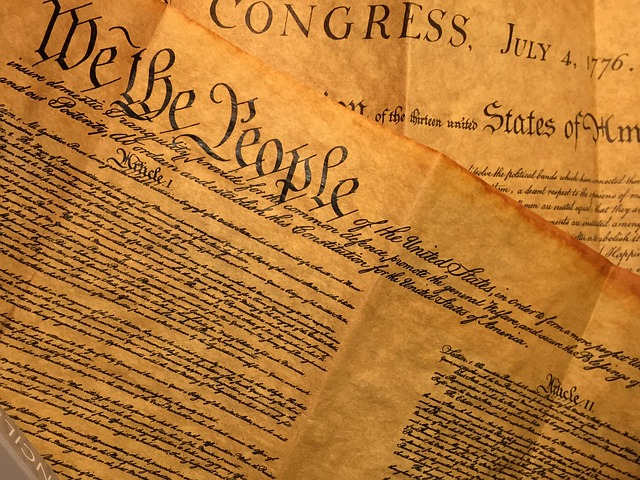
\includegraphics[width=0.5\textwidth,height=\textheight]{img/constitution.jpg}

\begin{centercap}

\href{https://pixabay.com/users/lynn0101-8308820/}{lyn0101} at Pixabay.com

\end{centercap}

\end{centerpic}

\begin{epigraph}

For it can never be that war shall preserve life, and peace destroy it.\\
~\\
---Thomas Hobbes, Leviathan

\end{epigraph}

\textbf{\emph{At this point we have considered}} five different approaches to understanding and explaining ethics -- Relativism, Divine Command Theory, Natural Law Theory, Psychological and Ethical Egoism. Each of these at first might have seemed to offer a reasonable account of the origins and nature of moral principles, or in the case of egoism of why moral principles are best ignored. But then each also turned out not to hold up very well to critical analysis. Let's briefly look back at what went wrong in each case, since maybe that might help us find a way to move forward in our quest to find a basis for morality and ethics.

\textbf{\emph{Relativism claimed}} that morality is nothing but a set of culturally dictated rules and that as a result of this, that there are no moral universals. Even if relativism may seem obvious to some people, in the end, it seems to overstate its case. Is there really no such thing as something that is just plain wrong? And does relativism really succeed in establishing that there really are no universal rules underlying particular cultural norms. If there are deeper common rules that transcend cultures, the relativistic claim that particular cultural rules are binding on us because there are no others would lose its force. And finally, relativism fails to provide a convincing answer to the question ``Why should I listen to what my culture tells me I should or shouldn't do?''

\textbf{\emph{Divine Command Theory,}} on the other hand, appealed directly to an authority that supposedly commands universal assent, God, as the basis for moral rules. But this theory ran into trouble as well, since it rested everything on an appeal to authority. The problem here is that simple appeals to authority fail to provide any reasons why we should follow the commands of even an absolute moral authority -- ``Is it because God commands me that I should follow the rules, or should I follow these rules because they are really the correct rules?'' Neither of these options really provide reasons to accept a set of rules -- the first says follow the rules or else, and the second says that there are reasons to follow the rules but fails to provide them. So we are left not really having any idea why we should bother following the rules.

\textbf{\emph{Next, natural Law Theory claimed}} that we should orient our lives according to what nature dictates by striving to fulfill our natural capacities and by avoiding anything ``unnatural'' that violates the natural functions built-in to our bodies and minds. Once again, however, this theory failed to provide a convincing reason for us to follow human nature. Even if we could all agree about what our natural capacities and functions really were, we can always still ask, ``But why should I do what my nature tells me I should do?'' Unlike other animals who have no choice but to follow their natures it is always an issue with us humans whether we should do what our instincts tell us to do or not.

\textbf{\emph{Psychological Egoism}} in contrast to these last theories, dismissed ethical rules are unrealistic. But it turned out to have little explanatory power and amounted to nothing but a cynical dismissal of ethics. Thus once again the question of why strive to be a good person reasserts itself.

\textbf{\emph{Finally Ethical Egoism}} attempted to show how ignoring ethical demands was in fact the best way to achieve the social good. This position, it turns out was not well defended, nor in the end did it even seem logically coherent. Here too we are left with an unanswered question -- if focusing on oneself is the best way to achieve the best outcome for all of us why should we even care about this outcome in the first place?

\textbf{\emph{I hope a pattern}} is becoming apparent here. Each of these theories tried to solve the problem of explaining and/or justifying moral principles with its claim to have found the source of the basic moral rules that govern our lives together in society (or in the case of egoism why such rules are beside the point). In spite of the differences between these sources of moral rules, however, all of these theories leave something out. They all fail to spell out why it is that we should listen to any rules in the first place. All assume that the job of ethical theory is simply to find the source of ethical rules and that once we have found it we are done. Now it might strike you that this is an unfair criticism of these theories since each of them does at least suggest a reason why we should comply with the rules. Why should we take culturally dictated rules seriously, or why we should listen to the commands of God or human nature, or build a society based on the powers of ``invisible hand'' of market driven competition? If we don't we will fail to fit in with those around us, or we will end up being punished by God, or we will fail to find the true fulfillment that Natural Law Theory claims we can only get by following our true natures, or we will act in a way that is counterproductive to a good social outcome.

\textbf{\emph{This is not enough, however,}} since wherever the demands to conform to any rules come from it is always possible just to ignore them. I can simply ignore my culture, God, human nature, and even the demands of me, myself and I if I want to. The rules of human conduct are not like the laws of nature, since they depend in a crucial way on \emph{choice.} Even rules that supposedly come from outside of us still depend for their existence as rules on something inside of us, our freely granted consent to follow them. And if this is true, it seems less important to figure out where the rules of society and morality come from than it is to address the question of what it is about those rules that would encourage us to comply with them in the first place. After all, rules that nobody felt any reason to comply with would automatically cease to be rules, as anyone who has had first hand experience of a child in her ``terrible twos'' knows all too well. A stubborn two year old who has just learned the power of the word ``no'' doesn't have to do anything at all, no matter who says so. Likewise with ethical rules, we can and should all ask, ``Why should I follow the rules in the first place?''

\textbf{\emph{Social Contract Theory}}, as our next approach to ethics is called, is an attempt to answer the question of why we should follow the rules of the social game when we have a choice not to. In contrast to all of the other theories we have looked at, it doesn't just assume that saying where these rules come from is enough to get them to stick. Instead it tries to explicitly ground the rules governing our social lives in our ability to make free choices.

\hypertarget{hobbes-and-the-invention-of-society}{%
\section{Hobbes and the Invention of Society}\label{hobbes-and-the-invention-of-society}}

\begin{epigraph}

To this war of every man against every man, this also in consequent; that nothing can be unjust. The notions of right and wrong, justice and injustice have there no place. Where there is no common power, there is no law, where no law, no injustice.\\
~\\
--- Thomas Hobbes, Leviathan

\end{epigraph}

\hypertarget{ethics-in-times-of-social-and-political-change}{%
\subsection*{Ethics in times of social and political change}\label{ethics-in-times-of-social-and-political-change}}


\textbf{\emph{Historically speaking}} the question of why and which rules to follow come to the forefront in times of great social and political change. Political revolutions, for example, take place when an old order breaks down and this happens when enough people no longer feel compelled to follow the rules of the old authorities, when the old authorities no longer seem legitimate. Thomas Hobbes (1588-1679) was one of the first philosophers to recognize this fact about social rules in part because he lived through a time of great social upheaval, the English Civil War of the 1640's. Traditionally English kings had commanded absolute authority and had even claimed that this authority was granted to them by God. But these claims made no difference if enough people were willing to go against the authority of the king by simply refusing to follow orders issued by the king and his agents. Hobbes' experiences of the complete social breakdown of the Civil War period and the eventual restoration of the deposed monarchy convinced Hobbes that all rules of society and morality were inherently conventional, or products of the choices of the members of any society.

\textbf{\emph{The problem for ethical theory}} for Hobbes thus shifts from that of answering the question ``what are the rules governing behavior?'' to that of answering the prior question ``why should we follow any rules at all?'' Hobbes also thinks that answering the second of these questions will give us important clues as to how to answer the first. If we can figure out what it is that encourages us to conform to social rules, we can also start to see what rules it is that we are mostly likely to accept as valid rules. This is the basic idea behind Social Contract Theory.

\hypertarget{the-state-of-nature}{%
\subsection*{The state of nature}\label{the-state-of-nature}}


\textbf{\emph{In order to answer}} the questions of why we should follow any rules at all and what those rules might be Hobbes asks us to engage in a mental exercise, a ``thought experiment.''\footnote{Note that I am here intentionally ignoring the difference between ethical rules that would regulate individual conduct and the rules that make up the social order -- the rule of law. Social contract theory historically was an attempt to legitimize political authority, or why governmental institutions and rules should be respected. However, it seems to me that the arguments given here apply more generally to any sort of rules of social interaction like ethical rules as well. Contemporary backers of SCT, such as David Gauthier tend to look at it as operating on this more general level as a theory of any sort of socially binding norms.} Suppose, he asks, that there were no rules, that we lived in what he calls a pre-social ``state of nature,'' in which all of us are free to pursue our own interests with no religious, legal, moral or other restrictions on our behavior. In such a situation would we have any reason to create and honor any rules limiting our freedom? Would we have any reason to respect other peoples' property, to keep our promises to them, to cooperate with each other at all? Well, if there were no binding rules limiting acceptable behavior, Hobbes answers, we would have no interest in cooperating with each other. If there were no rules limiting our treatment of each other we would do whatever we thought we could get away with in pursuit of our own interests. Furthermore, in such a state of nature, since we would lack the ability to work with each other to produce the things that we all need to have comfortable lives, we would all be faced with chronic shortages of the necessities for life. This would lead ultimately to a ``warre of all against all,'' in which those who thought they were stronger, smarter or more cunning would try to take advantage of others perceived to be weaker in one way or another. In the end, however, all of us would suffer and life in the state of nature, to cite Hobbes' famous description would be ``solitarie, poore, nastie, brutish and short.''

\textbf{\emph{So life without any social rules}} would clearly be a mess. Hobbes thinks that this follows from a thoroughly realistic picture of what human beings are like once we strip away all of the conventions of social life. It is not that we are all mean-spirited or intent on hurting others out of maliciousness. It is just that we all need to look after number one first, and without any universally accepted laws of social behavior, it is always better to be safe than sorry and aggressively pursue what is in our own best interests and this for the simple reason that nobody else can be trusted to care about our interests. Once we realize that this kind of individualistic pursuit of self-interest is leading us all down the path to chaos, however, Hobbes thinks it becomes equally obvious that we need to find a way out of this mess. Our lives literally depend on successfully departing from the state of nature and creating rules that will enable us to live with more security than we can possibly provide for ourselves in the state of nature. And this is, according to Social Contract Theory how we can account for the origins of morality among members of a species like us who are naturally interested in only pursuing their own interests. Thus, as Hobbes argues, if there were no ethical or moral rules governing our relations to others, we would still have a very powerful reason to create and follow such rules because, namely, life without them would be unbearable.

\textbf{\emph{I have already mentioned}} that Social Contract Theory claims not only that we should answer the question of why we should bother accepting any rules at all, but that by so doing we will be able to also answer the more substantial question of which particular rules are really the rules we should accept. Social Contract Theory not only offers us an account of what it is about moral rules in general that makes them acceptable, it also spells out what those rules would look like.

\hypertarget{the-social-contract}{%
\section{The social contract}\label{the-social-contract}}

\textbf{\emph{For Hobbes,}} as for other advocates of Social Contract Theory, the big problem of a life without binding moral rules is that cooperation between individuals is impossible. If I have no reason to keep my promises to you, then, should I be tempted to not deliver what I have promised to deliver, I won't bother. If I have no reason not to respect your property when I am in a position to take it for myself, I will just take it. If there is no reason why I should avoid endangering your well-being, when it is to my advantage to do so, I won't pay any attention to whether or not my actions hurt or even kill you. Since, however, it is just these failings that would make life in a state of nature unbearable to all of us, it seems like these are the kind of things we'd all be willing to create rules against. Since not keeping promises, stealing and recklessly endangering others are what we'd most like to escape from in a state of nature, then these are the kinds of things that our moral rules should forbid. Entering into a social contract is then just agreeing to abide by a certain set of rules that we can all accept such as agreeing to keep our promises, to tell the truth to each other, not to steal from each other, or endanger each others' lives for no good reason. These are all of the things each of us wants, so these are the kinds of rules we would all accept. And we should all be willing to give up our freedom to violate these rules, because otherwise life would be unbearable for us all. This suggests an argument for Social Contract Theory.

\begin{center}

\begin{argument}

Life would be unbearable without moral rules.\\
So we have a strong interest in developing and following a set of moral rules.\\
~\\
Hence moral rules are a product of human choices and are grounded in our common self-interest in creating and preserving social order.

\end{argument}

\end{center}

\textbf{\emph{Social rules,}} according this argument, are thus thoroughly conventional rules that are based on mutual self-interest. They are not based on human nature, God's commands or the dictates of some cultural tradition or other. Instead they are put in place in order to allow us to live together, to engage in cooperative tasks, to own property, and to be assured that others will not infringe on our basic needs. The rules, once enacted, create legally enforceable rights and duties and enable us to depart from the chaos of the state of nature once and for all. Or so it seems at least.

\hypertarget{why-should-we-follow-the-rules}{%
\section{\texorpdfstring{Why \emph{should} we follow the rules?}{Why should we follow the rules?}}\label{why-should-we-follow-the-rules}}

\textbf{\emph{Social contract theory}} is not free from difficulties. Of the two major problems facing it, the first is a lack of clarity concerning the status of the agreement that creates moral rules. Is this supposed to have been a real agreement between real people at some point in the past, or a hypothetical agreement about what people would agree to if they were faced with the task of creating moral rules from scratch. The second problem with has to do with its adequacy as a justification for moral rules in general. Granted that it shows we have a need for such rules, it fails to provide an adequate account of why we should bother to follow the rules when we have constant incentives to cheat.

\hypertarget{what-agreement}{%
\subsection*{What agreement?}\label{what-agreement}}


\textbf{\emph{This first problem}} facing Social Contract Theory has to do with its claim that the authority of the rules of the social game can only be based on the free and willing consent of those under the authority of these rules. If social rules are conventional rules, they can only be binding to those who have freely accepted the restrictions they impose on us. But most of us, who never lived in any situation remotely resembling Hobbes' state of nature, probably cannot remember ever being asked to endorse a social contract. Instead, we are born into a society with a set of rules already established and taken for granted as legitimate rules and we are asked simply to accept these rules. But then how could these rules really be binding on us if we were never asked whether or not they fit in with our ideas of what would serve our interests best? There are two standard ways of responding to this question.

\textbf{\emph{First we might say}} that although the social contract was in fact a real historical event establishing a set of conventional moral rules, once these rules have been set in place, they are no longer subject to debate or rejection. Our ancestors who lived in a state of nature were in a unique position to found a social order and, short of the kind of complete social breakdown that occurs during a civil war or political revolution, subsequent generations have no choice but to accept the rules authorized by the original parties to the social contract. Perhaps subsequent generations can tweak particular details of the rules of the social game, as has definitely happened, for example, concerning relations between men and women in the western world. But the basic rules that result in the creation of the social world in the first place must henceforth be taken as given.

\textbf{\emph{This response is,}} however, unsatisfactory and even threatens to undermine the very thing that seems unique about Social Contract Theory, its claim that social rules are inherently conventional and based on the free choices of those to whom they apply. That is, if only the original parties to the social contract are in a position to accept or reject some set of social rules, then these rules can count as conventional only for them and not for anyone born into a later generation. But this means that the social rules are just as arbitrary for later generations as they would be if given by a particular culture, by God, or by some conception of human nature.

\textbf{\emph{The second way}} to answer the question of why moral rules might be binding on us even if we have never explicitly approved of them starts by rejecting the idea that the social contract should be understood as a real historical event. Instead, the contract should be understood as a hypothetical contract reflecting what rules would be acceptable to free and rational agents if they were living in a pre-social state of nature. That is, the Social Contract Theory is to be recast as an idealized set of rules that any free and rational individuals would be logically compelled to accept in order to avoid the general types of problems that would plague their lives in the absence of such rules. Just like physicists idealize in their accounts of the laws of motion by talking about things like frictionless planes and perfectly elastic collisions, us philosophers are licensed to talk about the requirements of free and rational agents in general, regardless of the historical details of their lives since what we are after is an account of the sorts of rules we should accept. This approach is by and large the approach taken by the majority of contemporary philosophers who take Social Contract Theory seriously as a way of justifying social rules philosophically, and it does seem like a reasonable way to proceed.

\textbf{\emph{Thus let us accept}} that Social Contract Theory is not dependent on the claim that a real agreement is at the basis of currently existing social rules. Instead let us accept for the sake of argument that the social contract is a hypothetical device that enables us to talk about what rules would be acceptable to free and rational agents whoever they happen to be. We can now ask a more difficult question of this theory -- why would free and rational agents accept any rules at all that limit their options in the way moral rules do? Moral rules, we recall, should be understood as rules that might get in the way of self-interest. For example, if there is a moral rule against lying to others, this means that whether it suits us at the moment to lie is not important because the rule against lying should overrule our immediate interests. We have seen that Social Contract Theory is based on the idea that we can all agree that certain sorts of behavior should be restricted since they tend to lead to chaos if enough people engage in them. Thus it certainly seems like moral rules have an important role to play in our social lives.

\hypertarget{the-prisoners-dilemma}{%
\subsection*{The prisoners dilemma}\label{the-prisoners-dilemma}}


\textbf{\emph{We may wonder, however,}} whether Social Contract Theory goes far enough by pointing out how moral rules can serve our collective interests. What is to prevent us from accepting a set of rules as long as it does not get in the way of our individual interests but then ignoring the rules whenever it seems to us that it pays to do so? If moral rules are necessitated by the fact that we are essentially self-interested individuals but also need not appeal to anything besides self-interest, doesn't this make moral rules highly unstable?

\textbf{\emph{To see why}} this is the case, let us consider a famous puzzle often called called ``The Prisoner's Dilemma.'' This puzzle condenses into a very clear picture the fundamental problem of morality -- why should we trust each other when we are all constantly facing temptations to violate trust and why should we stick to the agreements we make when a situation presents itself where it is in our interest to violate them?

\textbf{\emph{Imagine that you and a partner}} in crime have just been arrested after a botched attempt to rob a convenience store. The police have reason to suspect that you two have also successfully robbed other stores in the area but lack sufficient evidence to convict you of these other robberies. Since the police chief has been taking a philosophy course he decides to present each of you the following offer in separate interrogation rooms:

\begin{quote}
We have reason to believe that you and your partner have been involved in a string of robberies around here and we would like to put at least one of you in jail for a long time. So if you cooperate with us by testifying against your partner, we are willing to make you a deal. If you testify against your partner and she stays quiet, you will go free and she will get a 10 year jail sentence. If both of you testify against each other then we will give you each 5 years in jail. On the other hand if both of you refuse to cooperate with us and keep your mouths shut, we can only hold you for 1 year for the attempted robbery yesterday. What is your decision?
\end{quote}

\textbf{\emph{Now suppose}} that you and your partner have already come to an agreement not to rat on each other in case the police try to convince you to do so with an offer like this. What should you do here? That is, what is the smartest thing to do in this case assuming that neither you nor your partner really wants to go to jail and will always opt for a shorter sentence? Is there even a rational solution to this puzzle? Is it better for you or your partner to stick to the agreement not to rat, or is it better to rat? (Note that there are no hidden negative payoffs here, such as, for example, the threat that your partner will take revenge on you later on if you rat since that would distort the puzzle the police have presented to you. Besides, we are assuming that if you testify against your partner, the police will reward you with a new identity through their witness protection program.)

\textbf{\emph{The problem here,}} is that you cannot be sure about what your partner will do, since she is being held in a separate interrogation room. All you have is her word that she will not rat on you, and all she has is your word that you will not rat on her. The way to find a solution to this puzzle is to recognize that there are really two possibilities for each of you and thus four possible combinations. Either you partner will keep quiet or your partner will rat on you, and likewise for you. We can arrange these possibilities in a ``payoff matrix'' like so:

\begin{longtable}[]{@{}ccc@{}}
\toprule
& I keep quiet & I rat\tabularnewline
\midrule
\endhead
you keep quiet & 1 year each & I go free, you get 5 years\tabularnewline
you rat & I get 5 years, you go free & 3 years each\tabularnewline
\bottomrule
\end{longtable}

\textbf{\emph{So if your partner keeps quiet,}} is it better for you to rat or to keep quiet? Well since you would get less time in jail if you ratted (no jail time versus 1 year for sticking to the agreement not to rat) than if you kept quiet, if your partner keeps quiet then you should rat. But what if your partner rats -- after all, you do not know what she will do -- which is better, ratting or keeping quiet? Well here again ratting gets you less time in jail since if you keep quiet while she rats you end up with 10 years in jail, while if you both rat, you'll only end up with 5 years behind bars. This is known in the jargon of ``game theory'' which studies strategic situations like this, as a dominant strategy, since no matter what your partner does it is always better for you to rat. Unfortunately, since your partner is thinking in exactly the same way as you are thinking, if both of you choose what clearly seems to be the best thing to do, you will both rat on each other and will end up with 5 years in jail each. Why couldn't you have just kept your mouths shut and gotten only one year in jail each? It would be nice if you could just trust your partner not to violate the agreement you have made, and this seems like it gets both of you the better deal. It's too bad that trust seems to be irrational here since it is always better to rat no matter what the other person does.

\textbf{\emph{Much has been written}} about the prisoner's dilemma as a model for certain kinds of basic social interactions. For our purposes here, I'd like to mention only two points. First, this kind of situation arises quite often in the real world, namely whenever we may make an agreement with each other to play by the rules but are constantly tempted to cheat for an immediate gain, in spite of the fact that cheating leads to an outcome that is worse if enough people do it.

\textbf{\emph{Think, for example,}} about the problem of over-fishing. All fishermen recognize that over-fishing depletes fish stocks and thus threatens their long term livelihood. So suppose the fishermen all get together and agree that it is in their best long term collective interests to limit their own catch. The question for each fisherman, as he sets out his nets, ``Should I stick to the agreement and not over-fish?'' He reasons like so: Well, I have no idea if the other fishermen will stick to our agreement. Suppose they do -- in that case my over-fishing won't hurt anyone else's long term livelihoods, but I will benefit by having more fish to sell. On the other hand, supposed they also over-fish -- in that case I would be a fool not to also over-fish since my short term benefits would be better if I did and there won't be any fishing for anyone after a few years of over-fishing, so my not over-fishing does nothing to protect my long term interests. So everyone, reasoning in a similar fashion over-fishes and depletes the resource that all need to survive. Why can't they all just stick to their agreement?

\textbf{\emph{This last example}} is an example of a ``many person prisoner's dilemma,'' also known as a ``free-rider problem'' or the ``tragedy of the commons.'' With a little reflection you will probably be able to come up with numerous other situations that exhibit the same logic. The prisoner's dilemma has thus earned the reputation of being a simple model illustrating a very real problem faced by social actors trying to coordinate their behavior in a way that secures their own long term interests, which is exactly what Social Contract Theory says moral rules are supposed to do.

\textbf{\emph{This brings me}} to the second point I want to make about the prisoner's dilemma, namely that it shows the ultimate weakness of Social Contract Theory as a justification for moral rules. Moral rules are supposed to be solutions to situations like prisoner's dilemmas, since in the state of nature we all act for the sake of our immediate short term gain and thus cannot coordinate our behavior in a way that leads to peace and security. But moral rules alone, in the form of voluntary agreements not to break the rules that you yourself have agreed to, are not enough to get out of prisoner's dilemmas. As we saw a moment ago, a promise to follow a rule that we ourselves can agree is a good idea is worthless given the ever present temptation to cheat in order to get a better outcome.

\hypertarget{slideshow-summary-6}{%
\section{Slideshow summary}\label{slideshow-summary-6}}

\begin{slideshow}Here is a slideshow summary which can be \href{https://gwmatthews.github.io/ethics-slideshows/07-phl210-slides.html}{viewed online}, \href{https://gwmatthews.github.io/ethics-slideshows/pdf/07-phl210-slides.pdf}{downloaded} or \href{https://gwmatthews.github.io/ethics-slideshows/pdf/07-phl210-handout.pdf}{printed}.

\end{slideshow}

\hypertarget{further-exploration-5}{%
\section*{Further exploration}\label{further-exploration-5}}


\href{https://www.investopedia.com/terms/p/prisoners-dilemma.asp}{Investopedia on the Prisoner's Dilemma}: perhaps this seems like an unlikely source for information about a philosophical theory. However, given that prisoner's dilemma-type situations arise all over the place in social life -- whenever we make agreements with others and then find ourselves tempted to ignore those agreements out of self-interest, it is not in fact unlikely at all.

\href{https://www.pnas.org/content/114/1/7}{The Tragedy of the Commons}: the tragedy of the commons is a name given by the philosopher Garrett Hardin to a collective version of the prisoner's dilemma in which all involved are tempted to overuse a commonly held or accessed resource for personal gain. This has clear implications for our fate as a species as is explained in this article from the National Academy of Sciences.

\hypertarget{utilitarianism}{%
\chapter{Utilitarianism}\label{utilitarianism}}

\begin{centerpic}


\includegraphics[width=0.5\textwidth,height=\textheight]{img/crowd.jpg}

\begin{centercap}

\href{https://pixabay.com/users/free-photos-242387/}{Free-Photos} at Pixabay.com

\end{centercap}

\end{centerpic}

\begin{epigraph}

Actions are right in proportion as they tend to promote happiness, wrong as they tend to produce the reverse of happiness.\\
~\\
---John Stuart Mill, Utilitarianism

\end{epigraph}

\textbf{\emph{So far we have examined}} a number of approaches, all of which are popular, but all of which have proven to be unsatisfactory in one way or another. This may lead you to wonder whether all of this philosophical analysis is really such a good idea. Shouldn't we have some results by now, after all of this investigation? Won't philosophers be capable of poking holes in every theory that comes along with their hyper-critical methods of analysis? The answer is a definite ``yes and no.'' Although no ethical theory that has been developed is entirely without problems and criticisms, there are a couple that seem pretty good, even to us skeptical philosophers. In this chapter we will consider one of these more promising theories. It is known as utilitarianism and was developed in its most explicit form in the 19th century by two British philosophers, Jeremy Bentham and John Stuart Mill. To situate this theory in relation to the theories we have already examined, consider the following case :

\begin{quote}
Fred is on his way to a job interview and happens to be running late. On his way to the bus station he happens to notice a small child apparently drowning in a pool. He quickly glances at his watch and realizes that if he does not hurry, he will miss his bus and will be very late for the job interview. Fred decides not stop and help. He catches the bus and not only makes it to the job interview on time, but gets the job.
\end{quote}

\textbf{\emph{Something is clearly}} wrong here. Fred should have stopped to help, even if it meant being late for the job interview. The simple reason he should have stopped was that someone else was in need of help. And the fact that this person was in need overrides his personal interest in getting to the interview on time. Now, in spite of how obvious this might seem, none of the theories we have considered so far can really account for this simple moral intuition. And this does not make them look very good as theories about our ethical obligations. Consider what each would say about this case:

\begin{itemize}
\tightlist
\item
  Relativism: ``Stop and help if your culture values helping strangers.''
\item
  Divine Command Theory: ``Stop to help if and only if God commands you do help strangers.''
\item
  Natural Law Theory: ``Stop to help if and only if it is part of human nature to help others.''
\item
  Psychological Egoism: ``Helping would be selfish anyway, do whatever suits you more.''
\item
  Ethical Egoism: ``Don't help since it is best to let people help themselves.''
\item
  Social Contract Theory: ``Stop to help because it is in your long term best interests to help others.''
\end{itemize}

\textbf{\emph{None of these approaches}} can account for what seems compelling about this case, that is, that we just should help in cases when someone is desperately in need and it would cost us comparatively little to help them. Their interests should count for us at least this much. This, in a sense, is the moral intuition that utilitarianism tries to account for. It is an explicit attempt to justify our normal, everyday, moral sense that we should take other people's interests seriously. Our systematic analysis of the varieties of egoism gives us a theoretical motive for considering this point -- if we can't defend selfishness shouldn't we at least try to see whether the case for moral concern for others does any better? But our humanity should give us a deeper reason for examining the nature and justification for this very ordinary feeling of moral concern that we should feel and expect others to feel as well.

\hypertarget{happiness-and-the-highest-good}{%
\section{Happiness and The Highest Good}\label{happiness-and-the-highest-good}}

\textbf{\emph{Utilitarianism is one}} of the major contemporary philosophical theories about the nature of and justification for ethical principles. It has its roots in the writings of the Scottish philosopher David Hume (1711-1776), although the name ``utilitarianism'' is most closely associated with the works of Jeremy Bentham (1748-1832) and John Stuart Mill (1806-1873).

Utilitarianism is an attempt to provide a rational basis for ethical decision making. It focuses on the consequences of actions and measures their value by the amount of good they do for whoever it is that is affected them. As Mill puts it,

\begin{quote}
Actions are right in proportion as they tend to promote happiness; wrong as they tend to produce the reverse of happiness.
\end{quote}

\textbf{\emph{``Whose happiness?''}} you may ask. ``Everybody's!'' the utilitarian would answer. The sophisticated moral theory developed by Bentham and Mill in defense of this simple point is what we will be examining further here.

\textbf{\emph{Both Bentham and Mill}} aim to make ethics into nothing less than a science of human happiness. This science starts out with a distinction that is important for ethical theories in general, a distinction between different types of value. Some things have a value only because they help to bring about other things of value. For example, a car is valuable to me since it helps me to get around easily. If I live in a place where owning a car is not necessary to get around, or it becomes prohibitively expensive because I cannot afford parking, gas or maintenance, then it loses this value. This type of value is known as ``instrumental value.'' Something has instrumental value if it allows me to realize other goals I have. On the other hand, some things just have value in themselves. For example, I may want a higher salary since the extra money will enable me to rent a bigger apartment and this in turn will make happier. But my quest for happiness itself is not for the sake of anything further. Being happy is something I want for its own sake and not for the sake of something else, unlike the bigger apartment or the salary increase, both of which I want for the sake of something else. Something that has value on its own, without its being valuable for something else has ``intrinsic value,'' as opposed to instrumental value. Utilitarianism starts with the claim that the only thing that has intrinsic value is happiness. Everything else of value is valuable to us to the extent that we believe it will help us to attain happiness. Happiness alone is something that is desirable for its own sake. Thus it may make sense to ask someone who takes on an extra job to earn more money why she needs or wants the extra money, but it makes no sense to ask someone why they want more happiness out of life. It is the one thing we are all striving for, even if we each have our own unique perspectives on exactly what will make us happy.

\textbf{\emph{Now the question}} arises, ``what is the best way to attain happiness?'' Is there a reliable, rational, ``scientific'' way to increase our happiness? Both Bentham and Mill answer that there indeed is a scientific way to attain happiness, and it is called ``maximizing utility.''

\textbf{\emph{Each of us}} has his/her own idea of what will lead to happiness, but in general we are all out to maximize happiness. Now every pleasurable thing that we strive for has a cost including time, money, effort, and/or opportunity costs. But, both benefits and costs are uncertain. So the rational way of attaining happiness is by getting as much satisfaction for as little cost as possible given the uncertainties involved. This is ``maximizing utility'' or the rational approach to happiness.

\textbf{\emph{The rational way}} to attain happiness is to strive to maximize utility by taking into account the costs and benefits (as well as their respective probabilities) of each possible choice we may have in a give situation. So far, we have only been speaking of the way each of might satisfy his or her own selfish desires. Both Bentham and Mill argued, however, this account can be the basis of ethics as well. If each of of is out to get the most pleasure for the least cost, then the ethical thing to do would be the course of action that enables the most people to satisfy their personal interests at the least cost. Ethical choices are choices that lead to the greatest overall utility.

\hypertarget{implications-of-utilitarianism}{%
\subsection*{Implications of utilitarianism}\label{implications-of-utilitarianism}}


\textbf{\emph{So what then,}} are the implications of utilitarianism? It has a number of positive implications. First, it makes ethics relevant to the real world, by defining ethical actions as those that have the best overall outcomes. Being ethical would not be a matter of personal conscience alone, but would be something that would be good for everyone. Second, the ethical nature of an action or a decision is something that could be measured. This idea was particularly attractive to Jeremy Bentham -- he was a strong advocate of legal reform and used as his criterion for evaluating laws the question of whether or not a given law was beneficial or harmful overall. Third, making ethical decisions would not require anything other than the ability to figure out how much our actions impact the interests of others. All of us are equally capable of adding up the expected good and bad results of our actions and deciding accordingly.

\textbf{\emph{On the other hand,}} there are negative implications to the theory as well. We will be considering these in greater detail in the next section and in the next chapter, since the final position we will look at in the theoretical part of the course, Kantian ethics, is an explicit attempt to avoid the pitfalls of the utilitarian approach. Three problems stand out. First, since utilitarians claim that the moral worth of an action depends on it having better consequences than the alternatives we may wonder how we can ever really determine these consequences when we are making a decision. Of course, some actions have obviously bad consequences, like tossing a burning cigarette butt into a dry field of tall grass. But can we really reliably predict the consequences of our actions in the majority of cases? After all, moral problems seem to arise in just those cases where it is not entirely clear what the best thing to do really is. In addition, as many large scale engineering projects have shown, determining whether the consequences of a decision are for the best or not in part depends on when you ask the question. For example, the building of dams as sources of cheap power may seem like nothing but a win-win situation, but the long term environmental consequences of such projects may end up costing more than the proponents of the project could foresee.

\textbf{\emph{Second,}} since utilitarianism depends on comparing the benefits and costs of different actions on everyone who is affected by those actions, it assumes that it is possible to compare the impact of one's actions on different people. But how can we do this? Is there one neutral standard of comparison that might reveal that, for example, person A gets 3 units of utility from action X and 5 units of utility from action Y, while person B gets 5 units of utility from action X and only 1 unit of utility from action Y?

\textbf{\emph{Finally,}} we have the problem that, if utilitarianism is correct, and the moral worth of an action is to be measured by the amount of good it does in the world, this seems to do away with the concept of rights. As long as an action leads to a sufficiently good outcome, anything goes. For example, suppose framing and executing an innocent person for murder would lead to great happiness for the whole of a community. As long as we could show that the benefits to everyone else outweigh the costs to this innocent person, a utilitarian would not have a problem with this. But, what about the rights of an innocent person not to be punished for a crime he or she did not commit? We will return to this question in the next chapter.

\textbf{\emph{In spite of some}} of the troubling consequences of utilitarianism, however, it remains a popular theory. Part of the reason for its popularity is the plausibility of the argument for this view. It it to this that we now turn.

\hypertarget{why-should-i-care}{%
\section{Why should I care?}\label{why-should-i-care}}

\textbf{\emph{The argument for utilitarianism}} is straightforward and might go like so:

\begin{center}

\begin{argument}

Everyone is out for the same thing -- happiness.\\
The rational approach to happiness is maximizing utility.\\
All of our interests count equally.\\
~\\
Thus we should all strive to maximize overall utility.

\end{argument}

\end{center}

\textbf{\emph{That is,}} given a standard set of assumptions about human motivation and rationality, and adding an explicitly ethical premise (the third), we get the result that we should all strive to get the best possible outcome for the greatest number of people. Utilitarians claim that this argument shows why it is that we should use the good that our actions do for whoever it is that is affected by them as a measure of their ethical value.

\textbf{\emph{So far,}} in our description of the position of utilitarianism, we have seen the grounds for buying the first two premises. The first of these claims is a straightforward, and pretty obvious, description of human behavior. The second depends on a pretty clear and uncontroversial theory of rational action. Acting rationally has to involve taking into account the costs of doing something and the probability of actually accomplishing it. So far so good, but these premises do not yet enable us to go beyond egoism. They are perfectly compatible with a complete lack of concern for others. The third premise goes well beyond anything that an egoist would accept and clearly calls for a more involved defense. The whole weight of utilitarianism rests on this claim.

\textbf{\emph{So far,}} we seem to be admitting that people only care about themselves and getting what they individually want. Yet ethics is supposed to be about concern for others, or at least taking others into account when you are making a decision. Utilitarians, however, insist that we can construct an ethics on the basis of what we have so far said about human motivation. So what we have to show next is that not only should we act with our own interests in mind, but we also have to have a compelling reason to take others into account. We can't just assume that others count; we have to demonstrate that ignoring others' interests is just not a rational option.

\textbf{\emph{Consider the following,}} somewhat absurd, example. Suppose I have 10 dollars and would like to entertain myself on a hot sunny afternoon. I come up with the following two possibilities:

\begin{enumerate}
\def\labelenumi{\arabic{enumi}.}
\tightlist
\item
  I could buy a ticket to go see a Hollywood action movie.
\item
  I could use the 10 dollars to buy a six pack of beer and then go up to my roof where there happen to be some bricks left over from the construction of the building. My plan would be to hang out and relax, enjoying the breeze, while occasionally throwing a brick down on to the crowded street below.
\end{enumerate}

\textbf{\emph{In case 1}} I'd get some relief from the heat and a little relief from my boredom. But this relief would only last for an hour and a half, and I'd have to sit though yet another typical Hollywood movie in which the good guys get the bad guys, with all of the usual predictable car chase and cliff hanging scenes and all of the usual dazzling but fake looking special effects. In short -- it just doesn't seem worth the money.

\textbf{\emph{In case 2}} instead of the fake explosions and chaos, blood and guts of a Hollywood movie I could see the real thing. Maybe there would be multiple vehicle accidents and perhaps even a gripping real life chase, involving me too. This certainly seems more cost effective, a way of getting the most for my entertainment dollar.

\textbf{\emph{The only problem here}} is of course that option 2 requires that I assume that nobody else's interests, or lives for that matter, really count. In this scenario I am considering only my own interests and treating others as if their pain and suffering just didn't matter. The question is then, do I have any way to defend my actions? Can I possibly come up with good reasons for believing that my interests mean more than the interests of the people whose lives I am putting at risk for the sake of entertainment? It is not enough here just to insist that the people I am endangering wouldn't want me to endanger them. This is because I may genuinely not care what they think of my actions. I am acting selfishly here as a matter of fact. The real issue is whether I can in any way rationally defend my selfishness. Well, can I?

\textbf{\emph{It seems like}} I can't. Of course I can act selfishly, but that's not the same as convincing others, who are potential victims of my selfishness, that I am justified in acting selfishly. But that seems very unlikely -- why should you, someone who has his or her own needs and interests agree to let me endanger you unless you were getting something in return? But if I am selfishly endangering you, then you are not getting anything, or at least enough, in return, so you'd have no reason to go along with my selfish schemes. Thus I cannot defend my own selfishness. And if I cannot do this, then I must accept the third premise of the argument for utilitarianism: ``All of our interests count equally.''

\textbf{\emph{Where is all}} of this leading? To the claim that we don't really have any good reason for denying that others count just as much as we do. Once we are convinced of this it is a short step to the basic principle of utilitarian ethics, other wise known as ``the principle of utility.'' This states that the right thing to do in any situation is to look at all of the available alternatives and choose the one that gets the most benefit for the most people, or that maximizes overall utility. All of morality boils down to this one simple principle: do whatever brings the most benefits and the least costs to the greatest amount of people. On the account of utilitarianism I have been developing here, this principle follows from the fact that none of us really has any good reason for denying that others count just as much as we do.

\textbf{\emph{This is perhaps}} not a surprising conclusion. After all, isn't accepting the idea that others' interests count just as much as ours do a requirement for looking at things from a moral point of view? If we cannot accept this, then we are simply not moral agents. Utilitarianism simply makes this idea explicit and defends it with a clear argument.

\hypertarget{problems-problems}{%
\section{Problems, Problems}\label{problems-problems}}

\textbf{\emph{The difficulties}} faced by utilitarianism are of two types -- technical problems that arise from its claim to be based on a scientific calculation of the costs and benefits of our actions and deeper questions about its status as a moral theory. We will look at each of these in turn in this section.

\hypertarget{technical-problems}{%
\subsection*{Technical problems}\label{technical-problems}}


\textbf{\emph{These issues}} have already briefly discussed these in the last section but they deserve further elaboration since they may end up being more serious than defenders of utilitarianism seem willing to admit. The problems I mentioned there were the problems of measuring and comparing happiness as well as the problem of determining what exactly the outcomes of our actions might be. At first glance these may seem relatively minor, but it seems to me that they begin to call into question the very claim of utilitarianism to be a viable theory.

\textbf{\emph{So the first question}} is, if utilitarianism claims that we can determine the moral worth of an action by the results of that action and measure those result by the amount of happiness that it produces we may wonder how exactly we might go about measuring that. Of course it may seem obvious that I know for myself whether I am happy or not, whether my needs have been met, whether I am better off than I previously was in a variety of circumstances. It may also seem to be the case that we can compare different people and determine that one person is happier or better off than another at least in general terms. But that already suggests a problem for utilitarianism -- how can we get beyond the somewhat vague and indefinite comparisons we might make in such a way as to support the claim that the calculation of costs and benefits can truly lead us to an objectively valid measure of moral worth for any particular situation we might face? Economists and other social scientists frequently face similar issues and so fall back on a convenient stand-in for happiness -- dollar value. When they examine human decision-making from a scientific standpoint they often ask people to choose which of two alternatives people would pay more for, or how much would be required to compensate them for their efforts in a given scenario. This works well enough in given scenarios but it seems to be limited to cases in which a monetary equivalent can be given and there are many situations in which monetary value is a poor substitute for other more qualitative valuations we might make. For example, how might we compare the long term, but not particularly intense satisfaction of seeing one's children graduate from college to a shorter term and more intense pleasure, like that one might get from going skydiving. Any attempt to find a single scale on which to make an objective comparison must seem completely arbitrary. Hence Jeremy Bentham's claim to have developed a ``felicific calculus'' that would enable us to calculate the precise quantity of happiness produced by any action invites parody, something with Bentham himself unwittingly provided with his convenient verse mnemonic:

\begin{quote}
Intense, long, speedy, fruitful -- Such Marks in pleasures and pains endure. Such pleasures seek if private be thy end: If it be public wide let them extend Such pains avoid whichever by thy view: If pains must come let them extend to few.\footnote{Jeremy Bentham, \emph{An Introduction to the Principles of Morals and Legislation} (Oxford: Clarendon Press, 1970)}
\end{quote}

\textbf{\emph{This brings up}} the related issue of how we might be able to compare the results of an action across different people. Do we just end up counting heads? Is there a survey we can give to everyone involved to determined how much people really enjoyed the results of our actions or not?

\textbf{\emph{The general problem}} here of determining the precise payoff of our decisions gets even worse when we think about when that payoff even occurs. After all the consequences of my actions continue to spread out in all kinds of ways like the ripples on a pond after you throw a stone into it and there seems to be no non-arbitrary way to determine when exactly the further consequences no longer need to be taken into account. It is not as if the consequences of our decisions simply stop being relevant after a certain definite point.

\textbf{\emph{And finally}} in this vein, we may wonder how it is that we can even tell what consequences our actions even may have. It seems to me to be no accident that the classic ``trolley problem'' where we are asked to decide whether to throw a switch that leads to the death of one person on one track as opposed to doing nothing causing the death of more than one person on another is cast on a railroad, where a speeding train car is locked into its trajectory. In the real world there are no such well-defined and pre-determined alternatives but instead we have to take at best educated guesses about what might happen as a result of our decisions.

\hypertarget{deeper-questions}{%
\subsection*{Deeper questions}\label{deeper-questions}}


\textbf{\emph{The deeper questions}} that utilitarianism faces have to do with its fundamental claim that we can and should define what is right in terms of what is good. Well can we and should we? As we will be seeing in more detail in the next chapter the philosopher Immanuel Kant argues that the answer is no. In the absence of his particular arguments about why this is the case we can here at least appeal to our moral intuitions. This isn't really a definitive proof that utilitarianism is wrong, but it does at least suggest that we need to look at things more carefully, which Kant will offer a way of doing.

\textbf{\emph{The big worry here}} is captured by the question, ``Can the ends ever justify the means?'' Utilitarians answer in the affirmative -- given good enough outcomes, the pursuit of the greatest happiness for the greatest number of people may in certain cases lead us to endorse doing things that seem to be morally dubious. Should we ever risk the lives of innocent people in order to accomplish a ``greater good?'' Well utilitarians might very well answer in the affirmative if they consider the payoff to be big enough. But then, if we can't really determine how big the payoff really is, how can we say when this might be the case? Are we really justified in causing real harm in the interests of avoiding even worse but merely hypothetical results if we acted differently. Since we have no real way of rewinding the tape and playing the scenario again with a different choice at the crucial moment we are basically reducing the morality of any given decision to something that is basically unknowable --- what would have happened if things had been otherwise. Real life examples of this are easy to find and it always must seem at least a little suspect to offer as a response to the victims of our actions, ``Trust me the outcome would have been much worse if I did this instead of that.''

\hypertarget{slideshow-summary-7}{%
\section{Slideshow Summary}\label{slideshow-summary-7}}

\begin{slideshow}Here is a slideshow summary which can be \href{https://gwmatthews.github.io/ethics-slideshows/08-phl210-slides.html}{viewed online}, \href{https://gwmatthews.github.io/ethics-slideshows/pdf/08-phl210-slides.pdf}{downloaded} or \href{https://gwmatthews.github.io/ethics-slideshows/pdf/08-phl210-handout.pdf}{printed}.

\end{slideshow}

\hypertarget{further-exploration-6}{%
\section*{Further exploration}\label{further-exploration-6}}


\hypertarget{kant-and-the-ethics-of-duty}{%
\chapter{Kant and the ethics of duty}\label{kant-and-the-ethics-of-duty}}

\begin{centerpic}


\includegraphics[width=0.55\textwidth,height=\textheight]{img/king-audacity.jpg}

\begin{centercap}

\href{https://www.flickr.com/photos/22711505@N05/}{Ron Cogswell}

\end{centercap}

\end{centerpic}

\begin{epigraph}

Two things fill the mind with ever-increasing wonder and awe, the more often and the more intensely the mind of thought is drawn to them: the starry heavens above me and the moral law within me.\\
~\\
---Immanuel Kant, Critique of Practical Reason

\end{epigraph}

\textbf{\emph{So far our discussion}} of ethical theory has revealed many different aspects of ethics. Each of the theories we have considered is, we might say, partly right and partly wrong about the nature of ethics. Each is partly right, since it captures some important feature of ethics, but partly wrong in that it chooses the wrong feature as the foundation for the rest. According to relativism, for example, the defining feature of ethics is its connection with culturally transmitted rules organizing our social lives. Resting the whole weight of ethics on this feature, however, leads to all of the problems we encountered in our investigation of relativism. The same holds for all of the other views we have considered, as can be seen in the following table.

\begin{longtable}[]{@{}ll@{}}
\toprule
theory & what it emphasizes\tabularnewline
\midrule
\endhead
Relativism & ethical rules as cultural norms\tabularnewline
Divine Command Theory & authoritative character of ethical rules\tabularnewline
Natural Law Theory & connection of ethics to human well-being\tabularnewline
Egoism & individuals always make their own decisions\tabularnewline
Social Contract Theory & legitimate rules grounded in rational choice\tabularnewline
Utilitarianism & ethics require impartial consideration of interests\tabularnewline
\bottomrule
\end{longtable}

\textbf{\emph{So each theory}} we have considered implies a judgment about what is really important about ethical decision-making. The final theory we shall consider, Kantian ethics, also makes such a judgment. For Kant, what is distinctive about ethics is contained in the concept of duty. Kantian ethics uses this concept as the foundation of ethics. As we shall see, there are some compelling reasons behind this approach to ethics, although, as we might suspect, some challenging consequences as well.

\textbf{\emph{We are all familiar}} with the word ``duty.'' A duty is something we simply ought to do, whether we want to or not. For example, if we have a duty to pay taxes, it really makes no difference if we can think of better things to do with the money, we simply have to get our tax forms in by the due date. (In fact the word ``due'' comes from the same root as the word ``duty'' both of which refer to what we owe, to our obligations.) Duty is an inherently normative concept and is thus likely to have some connection with ethics. But what exactly is the nature of that connection? Immanuel Kant (1724-1804) was a German philosopher who developed his approach to ethics as an attempt to answer this question. A more generic term for the ethics he developed is ``deontological ethics'' which literally means ``the ethics of duty,'' but since that is an awkward term, we'll stick with calling it Kantian ethics in honor of its founder.

\textbf{\emph{Kant's big question}} is this: what is the basis of the duties we may feel towards each other, ourselves and society? Is it based on the feelings of commitment we may have towards each other -- feelings of solidarity, sympathy, or affection? Or is there a rational basis for our duties -- can we become convinced that we have them and then act on them by thinking things through? Or are they based merely on fear of authority, the desire for self-preservation and getting what we need and want in a hostile and competitive world? Are we ``pushed'' to do certain things and avoid others by culture, God, human nature? Or are we ``pulled'' by what we want as individuals and groups? Or is there something else that can get us to do what it is that ethics claims we should or shouldn't do? Kant's answer, as we will see is that duties result from our ability to push ourselves by recognizing the binding and non-negotiable character of moral law. We are not moved by external forces, nor encouraged by inner desires when we act morally, instead we act \emph{autonomously}. We'll see what this means in more detail in a moment.

\hypertarget{what-do-we-owe-one-another}{%
\section{What do we owe one another?}\label{what-do-we-owe-one-another}}

\begin{epigraph}

In the kingdom of ends everything has either a price or a dignity. What has a price can be replaced by something else as its equivalent; what on the other hand is raised above all price and therefore admits of no equivalent has a dignity.\\
~\\
---Immanuel Kant, Groundwork of the Metaphysics of Morals

\end{epigraph}

\textbf{\emph{Philosophy is the art}} of making distinctions. If this is true of the work of any philosopher it is definitely true of Kant. The first and most important distinction to keep in mind as we start to explore Kantian ethics is that between the ``conditional'' and the ``unconditional.'' This distinction applies to claims about what is true or false (knowledge claims) as well as to claims about what is right and wrong (moral claims). As an example of something that is unconditionally true, consider the following claim from elementary geometry, ``For every right triangle with legs labeled a, b and the hypotenuse labeled c, the sum of the square of the legs a and b is exactly equal to the square of the hypotenuse c.'' It does not matter what the triangle is made of, whether it is drawn in a book, encoded in a computer program, sketched in dirt on the surface of the moon. This relation between the sides of a right triangle holds unconditionally. On the other hand, most of the (non-mathematical) claims that we make are at best conditionally true. For example, even though it is true that water boils at 100 degrees Celsius, this might not have been the case if the laws of physics and chemistry were different and it all depends on atmospheric pressure which is why high up in the mountains where there is less air pressure water boils at a lower temperature than at sea level. Likewise, that I was born to my particular parents on the day I was born is contingent, something that might not have been the case, and so it is only conditionally true that my birthday is when it is.

\textbf{\emph{The same distinction applies}} when we are talking about right and wrong. Some things are only conditionally right or wrong. It is, for example, wrong to drive on the right side of the road in England, since the accepted, and legally binding, norm is to drive on the left side of the road. But this clearly might not have been the case and in many other places in the world, one is expected to drive on the right. What about things that are unconditionally right or wrong? Are there any such things? Well in Kant's view unless we recognize that there are some things that are unconditionally right and unconditionally wrong we have failed to grasp the point of ethics. In fact, Kant's ethics is an extended defense of the claim that there are such things as unconditional duties, things that we simply either should do, or should avoid doing, no matter what. We will see what Kant's defense of this fairly strong claim looks like in a moment. Before we get there, let us take a look at what this claim implies about ethics.

\hypertarget{implications}{%
\subsection*{Implications}\label{implications}}


\textbf{\emph{So, then, what are}} the implications of the claim that there are such things as unconditional duties? First of all, this fits in very well with some basic moral intuitions that many people share, namely that some things are just plain wrong. There are some things that we should just simply never do, no matter what the benefits of doing them may be. For example, many people would agree that things like murder, rape, torture and slavery are simply wrong. (Remember that we are not committed to the truth of this claim just yet, since we still need to examine Kant's argument that this there really are unconditional duties.) Furthermore, if it in fact the case that such things should never be done, then this would enable us to flesh out the concept of ``rights.'' Rights are nothing but standards of treatment we are entitled to unconditionally. My right not to be tortured continues to hold, or should continue to hold according to Kantian ethics, no matter what might be gained for society as a whole by torturing me. If Kant is correct, then, and only then does the concept of rights really mean something.

\textbf{\emph{This position is clearly}} at odds with utilitarianism, according to which nothing should ever be ruled out as a possible course of action since it may be the best way of attaining the greater good. Utilitarians have to leave open the possibility of murder, rape, torture or slavery as avenues to getting the best for the most. This is the fundamental conflict between utilitarians and Kantians. This conflict, however, extends far beyond the question of rights. For Kantians ethics is not concerned with trying to attain the greater good for the simple reason that it is not concerned with attaining what is good. Ethics, in Kant's view is about doing what is right and not what is good. It might be nice if the people who did the right thing habitually were also rewarded with happiness for their efforts, but there is no guarantee that this will happen. Basing ethics on the contingent outcomes of our actions is sacrificing the truly ethical side of our actions for things that are utterly undependable.

\textbf{\emph{This goes back}} to one of the problems with utilitarianism mentioned in the last chapter, the problem of predicting the outcomes of our actions. Since according to utilitarianism, ethics requires choosing whatever leads to the best overall outcome, it assumes that the consequences or our actions are at least roughly predictable. But, as Kant points out, what happens in the world is contingent -- dependent on many things that are simply out of our control. So basing ethics on the contingent effects of our present choices seems hopelessly unreliable as a source of ethical guidance. By placing the ethical value of actions out in the world this value gets lost in the shuffle.

\hypertarget{persons-and-things}{%
\subsection*{Persons and things}\label{persons-and-things}}


\textbf{\emph{A second important distinction}} that follows from Kant's claim that there are such things as strict duties is the distinction between persons and things. Both persons and things have value, but the value each has is completely different. Things are valuable in that they are useful for our plans, they are means to an end. Their value is not inherent in them but in the other things of value that we get by means of them. As a result, the value of one thing can be compared to the value of another -- an idea reflected in the fact that we give a price to things thus showing how their value compares with the value of other things. Finally, the value of things can be used up. In the end, when a things ceases to be useful to us or even becomes a burden to us, we get rid of it or trade it for another thing. Persons on the other hand, have an entirely different sort of value. Their value is intrinsic or inherent and not dependent on their use for our projects -- that is, as log as we are treating them like persons and not like things to be used. Instead of having a price, a person has an inherent dignity, a moral worth that transcends what good they may do to us. Thus, the primary way we treat other persons should be respect. They are worthy of respect simply in recognition of their intrinsic value.

\textbf{\emph{Now all of this}} may sound completely idealistic and may seem to have little connection with the real ways in which we relate to each other. In Kant's view that just shows how little our behavior really corresponds to the standards of morality. The fact that we often fail to treat other people persons with inherent moral dignity has nothing at all to do with whether we should treat them like that. In fact, this basic distinction between persons and things follows directly from the idea that there are some things that are just plain wrong. What this really means is that there can never be an excuse for doing certain kinds of things to people. The ideal of moral treatment and the idea that there are real moral standards that just should not be violated are two sides of the same coin.

\hypertarget{rights-and-the-ideal-of-respect}{%
\section{Rights and the ideal of respect}\label{rights-and-the-ideal-of-respect}}

\textbf{\emph{Kant's claim}} that we should have absolute unconditional respect for persons will doubtless attract skeptical responses. Isn't respect something that has to be earned? Isn't respect conditional and can't we lose respect for others if they show by their actions that they are not worthy of respect? This is a tricky issue, but Kant would have to answer no to these questions. Respect is something that is owed unconditionally to all rational agents. There are two reasons why Kant takes this position. First, if respect is conditional -- if each of us will only grant respect to those who prove themselves worthy of respect -- respect would never get off of the ground. I would be waiting for others to begin respecting me while they are all waiting for me to begin respecting them. The only way to ever get respectful relations going is for someone to start respecting others with no strings attached. The second reason why Kant refuses to accept that respect is something that can be lost, comes from his recognition of the limitations inherent in our knowledge of each other. If I deem someone else not worthy of continued respect, I am essentially downgrading their status to that of a thing, something beneath me that I can dispose of or use at will. But who am I to make such a decision? How can I possibly claim to put myself in a position to be able to judge someone else like this? Perhaps God knows that the person I refuse to respect is not really worthy of being respected, but lacking such an absolute perspective on things, how could I ever decide that another person is really not worthy of respect? The only way I can do this is by assuming that I am somehow above the person I condemn. But that is an unjustified (and in fact immoral) assumption to make.

\textbf{\emph{As a result of these difficulties}} with turning respect into something conditional, we have no choice but to understand it as something unconditional. The moral point of view simply demands that we recognize certain absolute limits on the way we interact with others, including our willingness to judge the value of others. We must not put ourselves above other people, no matter how unworthy of respect they seem to be. But then, this should not seem to unusual, since it is exactly what it means to have rights. Rights are claims that we make about what sort of treatment we are each entitled to. And rights, if they are really rights, have to be unconditional, universal and inalienable. They have to be unconditional because, if they were not, they would be dependent on someone else's judgment about whether or not each of us deserves rights. But the whole point of insisting in rights is that nobody can be absolutely trusted to make such decisions. Historically, the concept of rights arose in the late 18th century, the era of the American and French revolutions. In those days absolute monarchs had the power to decide whether or not someone else was worthy of respect. But, as the colonists in what was to become the United States and the revolutionaries in France were very much aware, granting that sort of power to anyone undermines the security of everyone. So the ``Bill of Rights'' and the ``Declaration of the Rights of Human Beings,'' both insisted on the absolute non-negotiable character of rights. In addition, there is ultimately no way of containing rights to one group of people -- even though it took us Americans almost another 200 years to grant full political rights to women and non-whites, the idea of rights really only makes sense if it applies to all rational adults. Finally, rights, if they are to remain rights and not become something much weaker, must be inalienable -- incapable of being taken away. If they could be taken away, whoever is entrusted to taking some people's rights away would then be elevated an almost godlike stature above those whose rights are being taken away.

\hypertarget{conflicting-duties}{%
\subsection*{Conflicting duties}\label{conflicting-duties}}


\textbf{\emph{Kant's position on ethics}} is thus quite a bit more demanding than the other views we have considered. It insists on the absolutely binding character of moral rules. For some critics of Kantian ethics, this makes it seem too rigid to deal with real life situations that seem to defy clear definition in terms of right and wrong. The most obvious, and most frequently voiced, objection to Kant's insistence on the unconditional character of duties is that it seems to prevent us from being able to deal with cases where duties come into conflict with each other. For example, if someone shows up at your door and demands to know if your brother there, you are obligated to tell the truth, even if your brother is there hiding from this person and you suspect that he or she intends to harm your brother. It seems like our duty to help protect someone from harm and our duty to tell the truth come into conflict here. Most of us, naturally, would probably say that Kant is wrong in his insistence that we should tell the truth in this case, on the grounds that this lie is a good lie.

\textbf{\emph{But is there really}} such a thing as a ``good lie?'' According to utilitarians the answer is obvious -- as long a lying leads to a better outcome than telling the truth would have, the lie is good. Good lies are those with good consequences and bad lies are those with bad consequences. Of course, all of the problems with basing the rightness or wrongness of a decision on its consequences come rushing back in. How long do wait have to wait for consequences to unfold before we can decide whether it was worth it to lie or not? How do we measure the consequences of telling a lie in a way that is not subjectively biased towards our own interests? How can we compare the results of a real lie with what would have happened if we told the truth?

\textbf{\emph{In Kant's view,}} these problems demonstrate the utter arbitrariness of utilitarian approaches to ethics. But then what do we do when duties conflict? Well, Kant's answer is, that we have to try our hardest to fulfill all of our duties simultaneously, because we cannot rely on the usual utilitarian excuses to get us out of our moral commitments. So in the case of the person looking for your brother, you have to both tell the truth and protect your brother. Our duties cannot be overridden by what we think may or may not happen if we violate them. All of this assumes that we really have such unconditional duties. Thus we need to consider, at long last, Kant's argument that we really have such duties.

\hypertarget{the-categorical-imperative}{%
\section{The Categorical Imperative}\label{the-categorical-imperative}}

\textbf{\emph{So how is Kant}} going to try to defend the claim that we have strict, unconditional duties to each other? Earlier we considered the basic distinction between conditional and unconditional claims. Conditional claims are claims about what is right or true that may or may not hold. It all depends on circumstances. Unconditional claims must hold no matter what else is the case. It is, for example, unconditionally true that, say \(2 + 2 = 4\). That is, it does not matter what else is true, as long as we understand what it means to say that \(2 + 2 = 4\) we will see that it is true. But how do we show this? We prove it in one of two ways. First of all we could establish that it is true by reasoning validly from true premises about basic arithmetic and the definitions of numbers to show that it must be the case -- that is we can build a sound argument with \(2 + 2 = 4\) as the conclusion. On the other hand we could use a method known as ``indirect proof,'' and show that \(2 + 2 = 4\) must be true because denying its truth leads us to a contradiction. This is less obscure than it sounds. If I can show that it makes no sense -- that it entails a contradiction -- to say that \(2 +2 \neq 4\) then it must be true that \(2 + 2 = 4\). Kant realized that the same line of thinking applies to unconditional claims in ethics. If we have any unconditional duties, this can be shown by showing that denying these duties makes no sense at all, that it leads to a contradiction to do so. His basic argument in defense of unconditional duties is thus:

\begin{center}

\begin{argument}

If an action is to be morally acceptable its goal must make sense.\\
But some actions have goals that contradict themselves.\\
~\\
So such actions are unconditionally wrong and we have strict duties not to do them.

\end{argument}

\end{center}

\textbf{\emph{This argument is}} an extremely general argument. In fact we might consider it to be a kind of template for moral arguments in general, an argument schema that is to be turned into a moral argument be substituting particular actions for the general claims. Here is an example that shows why we have an unconditional duty not to steal:

\begin{center}

\begin{argument}

If stealing is to be moral its goal must make sense.\\
When I steal something, I do so in order to take possession of it.\\
But stealing undermines private property, since if everyone stole, there would be no such thing as private property.\\
Thus stealing has a contradictory goal -- it both assumes and undermines the possession of private property.\\
~\\
So stealing is unconditionally wrong and we have a strict duty not to steal.

\end{argument}

\end{center}

\textbf{\emph{The same general argument}} can be used to show that other things are immoral as well. Another example is lying. Why is it that lying is wrong? Is it because of the harm that lies cause as utilitarians might claim? Is it wrong to lie just because people lie are at risk of getting caught. Neither of these reasons come close, in Kant's view, to accounting for the moral status of lying. In his view, the following argument shows just why lying is wrong:

\begin{center}

\begin{argument}

If lying is to be moral its goal must make sense.\\
When I lie, I do so in the hope that others will believe my lie.\\
But lying undermines communication, since if everyone lied, there could be no reliable communication.\\
Thus lying has a contradictory goal -- it both assumes and undermines reliable communication.\\
~\\
So lying is unconditionally wrong and we have a strict duty not to lie.

\end{argument}

\end{center}

Likewise with murder. Murder is wrong, not because it causes pain (as utilitarians might argue), or because God commands us not to murder (as Divine Command Theory argues), but because the idea that murder could be acceptable contains an inner contradiction. The argument that it does runs like so:

\begin{center}

\begin{argument}

If murder is to be moral its goal must make sense.When I murder someone, I do so in the hope that my life will be better without that person around.\\
But murder undermines the possibility of having a good life, since if everyone murdered, nobody could live a happy and secure life.\\
Thus murder has a contradictory goal -- it both assumes and undermines the possibility of living a stable and secure life.\\
~\\
So murder is unconditionally wrong and we have a strict duty not to murder.

\end{argument}

\end{center}

\textbf{\emph{In all of these cases,}} the result is the same. Immoral action has ultimately irrational motives, motives that assume and undermine one and the same thing. Thus the only way to act immorally is presume a kind of double standard -- ``There is one set of standards that I expect everyone else to follow, but another set for me.''

\textbf{\emph{The argument for Kantian ethics}} is the most abstract of all of the arguments we have considered. And perhaps it seems to be stretching the limits of what reason alone can do as a method for grasping just what is wrong with immoral or unethical actions. Nevertheless, it seems to be at least a plausible argument, or set of arguments, since it seems to capture some important features of morality. First, morality does in fact seem to require consistency. If there is such a thing as morality, it would have to be the same for everyone, otherwise it would be nothing but an arbitrary set of rules lacking any ultimate basis. Second, Kant's argument makes it clear how morality can be universal, without being the kind of thing that one group can simply impose on other groups. To grasp the content of morality requires only thinking things through carefully enough to see that what I am doing either makes sense or fails to make sense when considered as something practiced universally. We certainly expect that every rational adult can grasp the fact that lying and stealing and murder just should not be done. Kant's theory shows us why we might be justified in having such expectations and in hold people responsible for seeing that ``you just shouldn't do those kinds of things.'' His theory certainly seems to impose some strict demands on us as moral agents, but then again, who said being good was easy?

\hypertarget{slideshow-summary-8}{%
\section{Slideshow Summary}\label{slideshow-summary-8}}

\begin{slideshow}Here is a slideshow summary which can be \href{https://gwmatthews.github.io/ethics-slideshows/09-phl210-slides.html}{viewed online}, \href{https://gwmatthews.github.io/ethics-slideshows/pdf/09-phl210-slides.pdf}{downloaded} or \href{https://gwmatthews.github.io/ethics-slideshows/pdf/09-phl210-handout.pdf}{printed}.

\end{slideshow}

\hypertarget{further-exploration-7}{%
\section*{Further exploration}\label{further-exploration-7}}


\hypertarget{part-applied-ethics}{%
\part{Applied Ethics}\label{part-applied-ethics}}

\hypertarget{theory-in-practice}{%
\chapter{Theory in Practice}\label{theory-in-practice}}

\begin{centerpic}


\includegraphics[width=0.55\textwidth,height=\textheight]{img/jizo.jpg}

\begin{centercap}

\href{https://pixabay.com/users/jordymeow-943760/}{Jordy Meow}

\end{centercap}

\end{centerpic}

\begin{epigraph}

In theory there is no difference between theory and practice, but in practice there is.\\
~\\
---Yogi Berra

\end{epigraph}

\textbf{\emph{At this point}} we have explored many different approaches to the fundamental questions of philosophical ethics. We have examined how these different approaches account for and justify basic moral principles and we have looked at how well-founded each of them was as a philosophical theory. But given such an abundance of theories we may be left wondering about how things might play out in real world cases where we have to make decisions about what exactly the right thing to do might be. Do we just pick whichever theory we like or which leads us to the results we want and then claim justification for our views? We could do that, but then that would require a willingness to leave out of account the various philosophical failings of many of the theories we have encountered. I won't rehearse these various failings here but in general I have tried to make the case that an adequate account of ethics must avoid two things. \textbf{\emph{First an adequate ethics}} cannot be based on appeals to some sort of external authority. Whether this appeal is to culture, God or nature doesn't really matter since all of these supposed sources of ethical norms inevitably leave us scratching our head and wondering \emph{why} exactly we should ever do what it is that they demand of us. It is always up to us as to whether or not to listen to any authority, and this depends crucially on what it is that we ourselves want.

\textbf{\emph{Secondly, however,}} ethics can also not simply be based on appealing to what it is that we want. Self-interest, whether in the crude and explicit form endorsed by egoism or in the more socially filtered versions at the basis of Social Contract Theory and Utilitarianism, is not in the end capable of giving us a reason to be ethical, since ethics involves putting our own interests aside, not for a greater payoff later but for another being now. Showing why we should ever do this and how we even can is the great challenge of philosophical ethics. This challenge is simply not met by showing how I can scratch my itches best by scratching yours, because sometimes that is just not possible. Morality can involve genuine sacrifice and renunciation of selfish desires and maybe even requires it in some cases.

\textbf{\emph{But then if ethics can't be based}} on what others want of us, nor on what we ourselves want, what on earth is left for it to be based on? Well, as I have tried to show in the last chapter, ethics might be based on something else, what we have \textbf{good reasons} to want in the first place. ``Reason'' here is not intended as some sort of mysterious force out there that is supposed to magically solve all of our problems, but simply as a shorthand for our ability and need to tell ourselves a truly convincing and coherent story about how we are living our lives. Reason is nothing but the demands that thinking beings make on themselves to live lives that harmonize, where we don't ignore inner contradictions in our intentions, where we don't neglect to consider the clash between what we expect for ourselves and require of others. This to my mind is the central insight of Kant's approach to ethics and also what is expressed in such more contemporary ideas as ``Universal Human Rights,'' and appeals to the unique dignity of moral agents. Kant agrees with Socrates that the unexamined human life is not worth living since it is not truly a human life failing as it does to live up to our capacity to reflect on and account for ourselves on terms that truly make sense to us ourselves. What Kant adds to Socrates is just some sense of how exactly we might proceed to examine ourselves and what constraints this self-examination imposes on how it is that we go about determining what exactly we should do.

\textbf{\emph{This is still, however,}} just a bare-bones account of what ethics really looks like because the real lives within which ethical decisions have to be made by us real people are messy and complicated. We still have to be able to put this general approach, as well as our knowledge of the inadequacies of the other various lines of thinking we have encountered into practice and this can be a hard thing to do. But practice requires practice and so the best thing is just start examining different kinds of situations and dilemmas that we may face in the real world and see what sense we can make of them given all we have seen so far, and that is what we will be doing in this part of the book.

\hypertarget{ethics-in-the-real-world}{%
\section{Ethics in the real world}\label{ethics-in-the-real-world}}

\begin{epigraph}

Debates about justice and rights are often, unavoidably, debates about the purpose of social institutions, the goods they allocate, and the virtues they honor and reward. Despite our best attempts to make law neutral on such questions, it may not be possible to say what's just without arguing about the nature of the good life.\\
~\\
---Michael Sandel, \emph{Justice}

\end{epigraph}

\textbf{\emph{As we proceed}} we should keep in mind what is at stake here. We are not simply looking for some technical means of solving problems once and for all. Instead the point of applied ethics is to develop our capacity to think about what it is that we consider a good life in the first place.

\textbf{\emph{In the succeeding chapters}} we will look at a number of topics in applied ethics in the light of the various theories we have been examining. It turns out that under the surface of many debates in applied ethics there are competing ethical theories and commitments. What makes these debates debates about ethics, and not policy debates about the pros and cons of some topic or other, is that both sides appeal to something that seems like it has a legitimate moral claim to our allegiance. In many cases the major arguments can be roughly divided between those that follow utilitarian ideas and those that appeal to Kantian ethical ideals and principles, but that is not always the case and the particularities of each topic often present obstacles to this simple dichotomy. We'll see how the different debates we have already examined on a purely theoretical basis play out for each topic.

\textbf{\emph{The particular topics}} we will examine are euthanasia; individual liberty and the legality of recreational drugs; crime and punishment; ethics and non-human animals; and environmental ethics. Each of these are huge topics and we will only be able to give a bare outline of some of the major ethical issues and argumentative strategies employed by backers of different sides of each issue. The point of this part of the book is to provide a brief overview of some of the major lines of argument in each case. It is my hope that this will be an inspiration for further exploration of these topics.

\hypertarget{euthanasia}{%
\chapter{Euthanasia}\label{euthanasia}}

\textbf{\emph{Our first topic}} in applied ethics is the topic of euthanasia (and/or physician assisted suicide -- these are not really the same thing, as we will be seeing shortly, although for convenience we will use the term ``euthanasia'' to cover both). The topic of euthanasia is not only a topic debated often in the public arena, but a central topic in the branch of ethics known as bio-medical ethics. The reasons for the importance of this topic are pretty obvious -- the debate about euthanasia arises from the dilemmas of aging and dying in a world in which medical technology often permits us to continue to live in spite of major medical problems brought on by aging, disease or misfortune. Modern medicine enables us to prolong life as never before, but in some cases prolongation of life ceases to be such an obviously good thing. So the question arises as to whether it is ethically permissible, in certain kinds of situations, to choose to die, to help others to die, or to even cause them to die.

\textbf{\emph{The word ``euthanasia''}} itself comes from two Greek words meaning literally ``good'' (\emph{eu}) and ``death'' (\emph{thanatos}). Some of the questions that arise in connection with euthanasia have to do with this literal meaning:

\begin{question}

\begin{itemize}
\tightlist
\item
  Is there any such thing as a good death, or is death just plain bad?
\item
  What exactly would constitute a good way to die?
\item
  Who, if anyone, can or should decide when the time is right for a human life to end?
\item
  Should medical professionals be involved in any way in decisions to end people's lives, or should they only be permitted to try to prolong life?
\end{itemize}

\end{question}

\textbf{\emph{The first three questions aside,}} for now, it is perhaps the last of these questions that has led to modern controversies about euthanasia. Modern medicine has given doctors enormous power to prolong life through radical surgical procedures and life sustaining technology that can keep some people in desperate medical conditions alive indefinitely. Thus medicine has had to confront a new dilemma: should doctors do whatever they possibly can to preserve life, in keeping with their traditional role, or should they accept moral limitations on this power to keep alive. Formerly doctors faced primarily technical limitations on what they could do, and so the chief moral responsibility they had was not to harm patients. But now that those limitations have been greatly reduced they find themselves face to face with questions about the value of life -- is it worthwhile to live whatever the cost in medical resources or individual suffering? Are there some lives that are no longer worth living, even though the technical means of extending them are available?

\hypertarget{types-of-euthanasia}{%
\section{Types of euthanasia}\label{types-of-euthanasia}}

\textbf{\emph{It is important,}} when we are discussing euthanasia, to be clear about what exactly we are talking about doing or allowing. For example, claiming that physicians should be allowed to assist terminally ill patients in ending their own lives is very different from advocating putting all mentally retarded infants to death, in spite of the fact that both could be considered forms of euthanasia. We can avoid some confusion by classifying types of euthanasia based on two separate factors, the degree of activity of the physician, and the degree of voluntary choice on the part of the patient. The role of the physician can be anything from that of a passive spectator doing nothing to assist a patient in continuing to live to that of an active agent causing the death of patient, (not to mention several possibilities in between). Patients, on the other hand can, voluntarily choose to die, or they may not be capable of making choices, or they may simply not want to die. (Don't be alarmed yet -- not all of these possibilities will lead to types of euthanasia that anybody wants to discuss. Some of them will be unethical or even criminal.) The following table lays out the relevant possibilities.

\begin{longtable}[]{@{}lccc@{}}
\toprule
patient's wishes / role of doctor & none & passive & active\tabularnewline
\midrule
\endhead
voluntary & suicide & DNR orders & Physician Assisted Suicide\tabularnewline
non-voluntary & accident & removing life support & hastening death\tabularnewline
involuntary & accident & negligence & murder\tabularnewline
\bottomrule
\end{longtable}

\textbf{\emph{Clearly this way of classifying}} euthanasia is just the beginning of the discussion. Some of these forms, such as passive voluntary euthanasia, are not at all controversial -- we have every right legally and morally to refuse medical treatment for ourselves. Implementing this right can be a problem, but the problem is typically one involving figuring out how voluntary a refusal of treatment really is, rather than the problem of whether or not someone should be allowed to refuse treatment. There are no real moral problems here simply because of the presumption that, as far as medical care is concerned, rational adults can decide for themselves about treatment of their illnesses and when enough is enough. On the other side of the scale, what the chart labels ``involuntary euthanasia'' is also lacking in any significant controversy, since killing someone or refusing treatment to someone against her will is clearly wrong. Nobody who is a serious participant in discussion about the ethical and legal status of euthanasia wants to defend involuntary cases. These must be mentioned, however, for two reasons. First, we need to distinguish non-voluntary cases, in which the patient has not or cannot express their desires in one way or another, from involuntary cases, in which the patient's wishes are being ignored or overridden. In other words, it is important to see that the opposite of voluntary may be involuntary or it may be non-voluntary. Second, mentioning involuntary euthanasia is important for historical and argumentative reasons -- the Nazi ``euthanasia'' program, the so-called T-4 program, was a program that killed over 100,000 unwilling victims and this specter of involuntary killing for supposedly medical reasons looms over the debate. As we will see, the danger that such a program presents is one of the motivations for the slippery slope argument against legalizing euthanasia.

\textbf{\emph{So the controversy}} about euthanasia is going to center around assisted suicide and active euthanasia, although as we will be seeing even suicide is subject to debate, as are cases of non-voluntary euthanasia. Assisted suicide has clearly been subject to many legal battles, those involving Jack Kevorkian, for example. It is currently legal in some parts of the United States including Oregon, which passed and implemented a law called the ``Death with Dignity Act'' in 1995. Active voluntary euthanasia, where, at the patient's request, a physician administers a lethal dose of a drug, is illegal in the entire country, although it is legal in the Netherlands and Belgium.

\hypertarget{arguing-about-euthanasia}{%
\section{Arguing About Euthanasia}\label{arguing-about-euthanasia}}

\textbf{\emph{The way I would like to assess}} these various types of euthanasia is by considering some of the major arguments for and against the different varieties of euthanasia. There are no doubt many other ways to argue about euthanasia than the arguments we will look at, but these are simply some of the better known and more worked-out arguments on the topic.

\hypertarget{against-medical-killing}{%
\subsection*{Against medical killing}\label{against-medical-killing}}


Our first argument is an argument against making any form of euthanasia, whether it is physician assisted suicide or active euthanasia, legal. It goes like so:

\begin{center}

\begin{argument}

The role of physicians is to aid in the preservation of life.\\
Legalizing physician assisted suicide or active euthanasia would require at least some doctors to violate that role.\\
~\\
Thus no form of euthanasia should be legalized.

\end{argument}

\end{center}

\textbf{\emph{At first glance,}} this may seem compelling. The Hippocratic oath, after all, mentions, ``First do no harm,'' as the primary constraint on the job of the physician. The primary role of medicine is, to add to the plausibility of this argument, to cure illness and relieve pain, and not to be involved in the termination of human life. However, on closer consideration, this approach to the topic of euthanasia soon reveals itself to be too general and inflexible to be of much use. First there are the technical issues involved in preserving life. For example, is a patient in an irreversible coma with severe and permanent brain damage really even alive? In a sense yes -- such a person has a heartbeat and can be kept alive indefinitely through the use of a feeding tube, and in a sense no -- no amount of treatment will be able to restore function to a brain permanently damaged by, say lack of oxygen. To say the least, cases like this make the role of the physician in preserving life quite difficult to understand and put into practice. In addition, this argument seems to lead to a blanket restriction on physicians playing any part whatsoever in the death of patients. But does this mean not giving palliative care, care intended to alleviate suffering, to terminally ill patients dying, say, of cancer? Medicine is not, in other words, always a struggle to maintain life, but is also often concerned with alleviating suffering. It is this additional role of the physician that is behind the second argument to consider -- the argument from mercy.

\hypertarget{appealing-to-mercy}{%
\subsection*{Appealing to mercy}\label{appealing-to-mercy}}


\textbf{\emph{The clearest argument}} in favor of legalizing at least physician assisted suicide and perhaps also active euthanasia appeals to the idea that we should ease the suffering of the terminally ill.~This is the other major role of medicine -- helping to relieve the suffering that disease or injury often entail.

\begin{center}

\begin{argument}

Some incurable illnesses cause immense suffering that medicine cannot relieve.\\
In such cases, preventing someone from dying sooner rather than later is wrong since it causes pointless suffering.\\
Allowing someone to kill themselves under a physician's guidance, or when necessary, allowing physicians to administer lethal drugs upon the patients request, is the only merciful option.\\
~\\
Thus physician assisted suicide, or even active euthanasia, should be legalized.

\end{argument}

\end{center}

\textbf{\emph{This argument clearly}} stands in contrast to the first argument, since it emphasizes the other aim of medical treatment, the alleviation of suffering. It insists, moreover, that it should be up to patients to determine whether or not their lives are ``worth it.'' So why not, it may be countered, allow patients to refuse treatment if they deem that their lives are no longer worth living? Well, in some cases, the suffering involved in a slow death is so bad, that it seems cruel not to allow patients to choose assistance in speeding the process up. (This point is central to Rachels' argument as we will see in a moment.) The argument from mercy rests on the assumption that someone can and should be allowed to give up on their own lives. That's obvious, isn't it? Well, not according to Kant.

\hypertarget{kants-argument}{%
\subsection*{Kant's argument}\label{kants-argument}}


\textbf{\emph{Part of the difficulty}} involved in discussing and resolving questions about euthanasia undoubtedly comes from the close relation between euthanasia (voluntary euthanasia at least) and suicide. Suicide has long been a taboo in Western culture, as it is in many other cultures. Suicide is held to be shameful, cowardly, an insult to others towards whom the suicide has responsibilities and/or to God (or the gods). It is a sign of a basic inability to cope with reality. Opponents of euthanasia often emphasize the connection of voluntary euthanasia with suicide. On this view, the person who opts out of struggling to survive a painful illness, or signs a do not resuscitate order is giving up hope and taking the easy way out. Thus as long as suicide is a taboo, voluntary euthanasia, if it is a form of suicide, would clearly also be off limits, not a topic to talk about in polite company, and certainly nothing to seriously consider as a rational response to illness.

\textbf{\emph{On the other hand}} there have always been defenders of suicide, not as something to encourage, but as a possibly rational solution to certain types of problems. The 18th century Scottish philosopher David Hume, one of the precursors of utilitarianism, wrote a famous essay in defense of suicide. In it he argued that killing oneself in certain circumstances could be rational or even obligatory if the only alternative was to bring harm upon others or suffer needlessly from a painful terminal illness. Kant, in contrast argues that suicide can never be rational, and so, according to his standard method of argument, it cannot be moral.

\begin{center}

\begin{argument}

An act can be rational only if performing that act does not undermine the possibility of attaining the goal towards which it is directed.\\
Suicide is a self-undermining act, since the point of suicide is relief from suffering, but the result of suicide is death -- a condition in which there is neither suffering nor relief.\\
~\\
So suicide is irrational and hence immoral.

\end{argument}

\end{center}

\textbf{\emph{According to this argument,}} suicide can never be defended as a moral act, and thus it should be ruled out of consideration in all cases. The problem here, of course, as utilitarian critics of Kant will be sure to note, is that it seems hopelessly unrealistic to judge the real-life complications of the end of a human life according to an absolute moral standard that insists that we all have a duty to struggle on in pain, no matter how awful it is. Nevertheless, Kant's claim that suicide is irrational in its intentions should give us pause, and keep up from the easy adoption of the attitude that ending one's own life is ever a purely rational choice.

\hypertarget{active-and-passive-is-there-a-moral-difference}{%
\subsection*{Active and passive, is there a moral difference?}\label{active-and-passive-is-there-a-moral-difference}}


\textbf{\emph{It is a very widely held belief}} that there is absolutely nothing wrong with voluntary passive euthanasia. Writing a living will and demanding that it be respected does not involve taking any moral risks, and is something that is perfectly legal in all fifty states in the USA, and throughout much of the world. Each of us has the right to refuse medical treatment and thus there is absolutely nothing wrong with asking doctors to stand back and allow us to die in certain circumstances. On the other hand, many people, perhaps even the majority, are opposed to active euthanasia, and assisted suicide. Requiring that doctors passively let us die, at our own request, is one thing, asking them to actually help us to do so is something else entirely. Or is it? James Rachels, in a well known article claims that this moral distinction between letting someone die (acceptable in some cases) and actively killing someone (unacceptable in most cases) does not stand up to scrutiny. In fact he argues that there is no moral difference between actively killing someone and passively letting them die. His argument is based on consideration of a fictional and somewhat implausible case, that of Smith and Jones, both of whom have rich uncles whose money they will inherit. Both Smith and Jones, morally corrupt as they are, decide that they do not want to wait for their uncles to die of natural causes, that is, they decide to kill their uncles.

\begin{center}

\begin{example}
\protect\hypertarget{exm:unlabeled-div-1}{}\label{exm:unlabeled-div-1}

Jones goes to visit his uncle, who is upstairs at home taking a bath and does not hear Jones come in. Jones, after having picked up a brick outside, creeps in and the up the stairs. He quietly opens the bathroom door and knocks his uncle on the head with the brick. Jones' uncle is knocked unconscious and sinks into the tub where he drowns. Smith, likewise, pays a visit to his uncle, grabs a brick from outside and creeps up to the bathroom where his uncle, as luck may have it, is also taking a bath. Just as Smith is about to kill him, however, his uncle bumps his head on the soap dish, gets knocked unconscious and thus drowns while Smith silently watches.

\end{example}

\end{center}

\textbf{\emph{Considering the details of this case,}} it seems that both Jones and Smith are evil people. Further, their acts seem equally bad -- both stand to gain from their respective uncles' death, both decide to kill their uncles, both approach them to carry out this intention. But only Jones' brick actually make contact with his uncle's head, while Smith's brick hovers a short distance above his uncle's head. But that seems like a completely inconsequential detail. So what if all Smith did was watch his uncle die, he is just as bad as Jones. Now the point of this case is just to show that in and of themselves, removing all other factors, killing and letting die are morally equivalent. In this case they are equivalently bad. As Rachels argues, in the case of euthanasia, if we accept that passive voluntary euthanasia can be a good thing, then active euthanasia in the same circumstances would be just as good.

\textbf{\emph{If there is no essential moral difference}} between killing and letting die then there is no way to defend the position that passive euthanasia is acceptable while active euthanasia is not. The Jones and Smith case shows that there is no essential moral difference between killing and letting die. Thus we should either allow both active and passive euthanasia or forbid both. This seems like a pretty compelling argument. Is there really any way to distinguish active killing and passive letting die? If not then their moral status, whatever it might happen to be, would have to be the same.

\hypertarget{peter-singers-argument}{%
\subsection*{Peter Singer's argument}\label{peter-singers-argument}}


\begin{center}

\begin{argument}

Some people have absolutely no hope for survival for medical reasons -- for example, babies born with anencephaly.\\
There are two choices in such cases, either they can be allowed to die naturally, or they can be painlessly killed.\\
Medical resources are limited.\\
~\\
Rather than waste medical resources on allowing anencephalic babies to die slowly, they should be killed to free up the medical resources where they will do some good.

\end{argument}

\end{center}

\textbf{\emph{In this argument,}} developed by Peter Singer, the claim is that in some very rare cases active non-voluntary euthanasia can be acceptable. These cases would be very clearly defined cases where there is absolutely no hope for someone, and yet allowing them to die (which will inevitably happen), as opposed to speeding up the process, prevents other people from getting the medical attention that they need. In such cases people should be killed in order to enable others to benefit from medical resources, such as hospital beds, IV drips, etc., that others might benefit from. Clearly this kind of argument is going to ruffle some feathers. But isn't it true that if we are devoting any resources to someone who has absolutely no chance of survival (and who is also not capable of being even conscious, as is true of anencephalic babies), that is a waste of those resources?

\hypertarget{slippery-slopes}{%
\subsection*{Slippery slopes?}\label{slippery-slopes}}


\textbf{\emph{Naturally, arguments like Singer's}} raise the question of whether even thinking seriously about killing any babies, no matter how hopeless their cases may be, is already going too far. Isn't this just disrespectful of human life, to contemplate throwing it away, however damaged it may be? And doesn't this kind of disrespect of human life often lead to disrespect for people with less severe afflictions? That is, are we not sliding down a slippery slope, if we accept Singer's argument? This brings up a standard objection to all varieties of euthanasia that are not currently acceptable, that is to anything stronger than passive voluntary euthanasia.

\begin{center}

\begin{argument}

Legalizing assisted suicide or active euthanasia will lead inevitably to the following consequences:\\

\begin{itemize}
\tightlist
\item
  Elderly people will give up hope sooner than they would if they did not have the opportunity to kill themselves or request euthanasia.
\item
  Those who pay for expensive treatments will put pressure on patients to choose death.
\item
  Doctors will lose a degree of respect for human life and will give up sooner.\\
\end{itemize}

All of these consequences are unacceptable.\\
~\\
Thus neither physician assisted suicide nor active euthanasia should be legalized.

\end{argument}

\end{center}

\textbf{\emph{In general,}} slippery slope arguments are not to be trusted -- ``\protect\hyperlink{slippery-slope}{slippery slope}'' is the name of a fallacy because the fact that one thing happens does not logically require that something worse will happen, if there is no law of nature that forces it to happen. There clearly is no law of nature that would force us to carry out involuntary euthanasia just because we happen to have legalized physician assisted suicide. As philosophers put it, there is no nomic or law-like necessity here. But, nevertheless, we may wonder whether doing something that seems innocent may not end up having long term detrimental consequences. The slippery slope argument at least demands that we take this possibility seriously.

\hypertarget{liberty-and-its-limits}{%
\chapter{Liberty and its Limits}\label{liberty-and-its-limits}}

\textbf{\emph{As we have seen}} in a variety of contexts, one way of understanding ethics is as an attempt to justify certain restrictions on our freedom. In general freedom is a good thing. But then there are some things that we just shouldn't do. The most obvious things we shouldn't do are things that involve deliberately hurting others. For example we would think that a bus driver who deliberately ran his bus full of passengers off of the side of a cliff did something that he shouldn't have done. It also seems clear that he would be morally and legally responsible for hurting others if he were to get drunk before showing up for work as a bus driver since he would be endangering the lives of the passengers as well as of other people who happened to be driving on the road with him. In such cases we seem to have every right to restrict the driver's freedom to do things like this. But what if this same driver decides to risk his own life by driving alone across a vast road-less area of the Sahara desert without enough fuel in the bus? Or what if he decides to get drunk while driving alone across the uninhabited desert where no one besides himself could possibly get hurt? These two cases might be cases of just plain stupid behavior, but can we, or should we, be able to restrict his behavior simply on the grounds that he himself might get hurt? These kinds of questions are at the root of the current controversy about the use of illicit drugs. Depending on how we would answer them, we will either end up siding with one of two different positions: libertarianism or paternalism. Libertarianism is the view that we should have the maximum amount of individual liberty possible -- whatever we see fit to do, for whatever reasons, we should be permitted to do, as long as it harms nobody but ourselves. Paternalism, on the other hand, is the view that we need protection from ourselves and that there are others, such as experts, legislators and policy-makers, who know what is best for us, and should decide for us the limits of our individual liberty even in such cases where we are the only ones likely to get hurt.

\textbf{\emph{One way to address}} these alternatives is in terms of a number of different principles for limiting liberty. These principles have been endorsed by various philosophers and political thinkers over the centuries.

\begin{itemize}
\tightlist
\item
  \textbf{The harm principle}: originally proposed by John Stuart Mill, this principle states that the only permissible limitations on liberty should be those that prevent us from directly harming others. Thus, although it would be wrong for me to practice my target shooting in a very crowded part of Boston, it would be acceptable for me to experiment with the injection of household chemicals into my veins according to the harm principle. Libertarians accept this view since it allows for the greatest amount of liberty.
\item
  \textbf{The social harm principle}: a more restrictive principle that is based on the recognition that we can harm others in indirect ways through the impact of our actions on society as a whole. Thus it may be socially harmful, and so, according to this principle at least, wrong, to sell pornography to consenting adults if it were to be shown that the sale of pornography encourages domestic abuse on the part of the purchaser, even if in some particular cases there is no abuse.
\item
  \textbf{The personal harm principle}: a yet more restrictive view that claims that it is wrong to use your liberty in ways that hurt oneself. Paternalists endorse this principle claiming that it is wrong to deliberately do things to oneself that it would be wrong to do to others.
\item
  \textbf{The offense principle}: the most restrictive view, which claims that it is wrong to exercise one's liberty in ways that cause offense to others. For example, it would be wrong for a woman to wear skimpy clothes in public if the local population is sufficiently conservative, or wrong to use language in a manner that people within earshot would find offensive. In spite of the restrictive character of this last principle, it does not necessarily capture the view of paternalists since it makes no mention of harm to oneself as being inherently offensive to others. Extreme social conservatives might adopt this view.
\end{itemize}

\hypertarget{libertarians-and-paternalists}{%
\section{Libertarians and paternalists}\label{libertarians-and-paternalists}}

\textbf{\emph{Libertarianism}} is the view that claims that we have no right to prevent someone else from engaging in risky, dangerous or disgusting behavior as long as it is clear that no one else will be hurt by that behavior besides the person engaging in it. In other words, libertarians argue that the state has no right to prevent me from riding a motorcycle without a helmet, watching pornographic videos in the privacy of my own home, injecting myself with whatever substances I feel like, as long as no one else is hurt by what I do. Even if I do things that are patently stupid, and clearly go against my own best long term interests, it is up to me whether or not I do them.

\textbf{\emph{The bottom}} line for libertarians is liberty. In their view liberty is what makes human life worth living, and it needs to be protected from arbitrary limitation. In the view of libertarians, unless it is clear that what I am doing infringes on your liberty or harms or sets back your interests, it should be up to me to decide what to do with my life. Libertarians defend this view by appeal to the benefits, both individual and social, of allowing as much liberty as possible. A society that allows as much liberty as possible may at times seem chaotic, but it is also a society in which individuals can find personal satisfaction in whatever way they see fit and in which society as a whole benefits from the innovations and new ideas that only free individuals can create.

\textbf{\emph{Paternalism}}, in contrast, is the view that it is acceptable to restrict others behavior even when what they are doing hurts only themselves. Paternalists believe that even mature adults need protection against our own impulses at times.

\textbf{\emph{Paternalists thus make the assumption}} that we are not always competent judges of our own interests. Left to our own devices we would degrade ourselves with drugs just for the sake of the cheap thrills they bring, we would gamble away our life savings in pursuit of the easy money of winning the jackpot, we would endanger our lives by taking stupid risks for the sake of the fleeting pleasure of riding a motorcycle with the wind in our hair. That is, paternalists are not confident that the average adult can in fact make rational, adult-like decisions about his or her own life. Thus, they believe that strong social sanctions, like laws regulating intoxicating substances, gambling, prostitution, etc. can be good things. Even though such laws limit our liberty, without them both individuals and society as a whole would needlessly suffer from self-abuse and degradation.

\hypertarget{the-case-of-recreational-drugs}{%
\section{The Case of Recreational Drugs}\label{the-case-of-recreational-drugs}}

\textbf{\emph{The debate between these two perspectives}}, libertarianism and paternalism, underlies a particular question that many societies have been grappling with in recent decades, that of the legal status of certain intoxicating substances or ``drugs.'' I this section we'll see how this debate plays out by examining a number of different arguments that have been brought forward either against legalizing the recreational use of drugs or in favor of it. As more and more states in the United States have legalized the recreational use of marijuana in recent years, these arguments have come into prominence and I am sure all of them will seem familiar.

\hypertarget{against-legalization}{%
\subsection*{Against legalization}\label{against-legalization}}


\textbf{\emph{There are a number of arguments}} that are typically given against the legalization of certain controlled substances that are currently prohibited for recreational use. I'll consider three of the most commonly given ones here. All three are often used to justify official federal policy in the USA and other countries as well and all have been challenged by states and countries that have recently legalized the recreational use of marijuana.

\begin{center}

\begin{argument}

The use of drugs for recreational purposes is in itself wrong.\\
In addition it has a corrupting effect on non-users when some people use drugs.\\
One of the roles of law is promoting public and moral order.\\

So currently illegal drugs should remain illegal.

\end{argument}

\end{center}

\textbf{\emph{This argument no doubt}} raises controversial points. Is the recreational use of drugs in itself wrong? If so, why exactly is it wrong? It would seem that utilitarianism would reject this idea, insofar as the recreational use of drugs might be pleasurable. A Kantian might perhaps see the recreational use of drugs as a violation of one's duty to oneself to live up to one's potential, but only if this use interferes with one's larger goals and aspirations. Certainly an occasional user need not undermine her life's projects by smoking or drinking every once in a while. So what moral theory does this claim then depend on? It seems like it might appeal to some conception of moral virtue, as developed by Natural Law Theory, since the use of drugs could be looked at a moral failing that indicates having a weak will or an inability to deal with life's problems and a willingness to seek an easy escape from those problems. But, as we saw in the earlier, Natural Law Theory faces some serious problems as an account of right and wrong. It grants too small a role to human freedom and choice in determining right and wrong and assumes that it makes sense to impose a single ``template'' of what morally correct action must look like on all of us. Hence this approach seems to many people to be suspect.

\textbf{\emph{On the other hand}}, suppose it were true that the recreational use of drugs was inherently wrong from a moral perspective, what then? Does it follow that because it is wrong it should thus be illegal? It almost seems to be taken for granted in official policy making circles that this is the case. But is it? Is the role of the criminal law to police public morality? Is that were the case, why are some ``vices'' such as smoking tobacco, watching pornographic videos, and the consumption of alcohol tolerated and others, such as the use of drugs such as marijuana and cocaine forbidden? We will return to this question of consistency in more detail later. For now, we can just state as an objection to this first argument, that the fact of something being wrong from a moral perspective alone wouldn't necessarily be enough to warrant its being made illegal. We live in a society that takes individual liberty seriously and separates ``private'' moral concerns from ``public'' legal concerns. The next argument, however, considers in greater detail the issue of broader, more public social harm suggested by the second premise of this first argument.

\textbf{\emph{Our next argument}} is similar to the previous one in that it assumes that the use of certain substances (so-called ``hard drugs'' -- basically anything more serious than marijuana) is either wrong or at least personally and also socially a very risky thing to do. But it also an argument that has been used against those who claim that marijuana is different than other drugs, since it is physically less harmful and generally less debilitating in its effects on the user, and so should be legalized.

\begin{center}

\begin{argument}

People who smoke marijuana at a young age are more likely than people who don't to use harder drugs later in life.\\
If we legalize marijuana more people will smoke it at a younger age.\\
So legalizing marijuana will increase the use of hard drugs.\\
The use of hard drugs is wrong and/or poses great public risks.\\

So marijuana should not be legalized.

\end{argument}

\end{center}

\textbf{\emph{This argument}} is the familiar ``gateway drug'' argument. It is often simply assumed in debates about drug use that marijuana is in fact a ``gateway drug,'' as in the familiar claim I saw recently in a video on the debate about drugs, ``drug counselors consider marijuana to be a gateway drug.'' The issue here has to do with what exactly it means to be a ``gateway drug.'' If it means that in fact people who use hard drugs like cocaine and heroin have most likely used marijuana prior to having used heroin or cocaine then it is obviously true that marijuana is a gateway drug. After all, most heroin users do not start out with injecting heroin into their veins. They probably started drinking alcohol and then moved on up the scale of more serious drugs that provide a more powerful effect. But this is not enough to get the argument off the ground, since what it needs is a relationship of cause and effect. It is because you use marijuana that you are much more likely to use other drugs later -- that is the claim that is being made in the argument. But is that true? Doesn't this look suspiciously like a case of the ``false cause'' fallacy? It is clearly true that marijuana users are more likely to use heroin that non-marijuana users, but that does not by itself mean that marijuana use \emph{causes} heroin use. That would be like saying that because the sun arises shortly after my alarm clock goes off every day, then the clock's going off must cause the sun to rise. In fact, the causal relation between marijuana use and heroin use is undermined even more by a simple fact about usage rates. Even though large numbers of people have smoke marijuana on a regular basis, many fewer are regular heroin users. But if marijuana \emph{caused} heroin use, shouldn't the numbers of heroin users be significantly higher? Compare the claim that smoking causes cancer -- if only one percent of smokers ended up with cancer, then this claim would clearly seem to be stretching the evidence. So then, how do we explain why non-marijuana users are far less likely to use heroin than marijuana users? It seems clear that there may be some common third factor that is the cause of both. Perhaps I have a physiological weakness for addictive substances, or come from a background that leads me to drug use in general. Whatever the case may be, whether it is nature or nurture that leads me astray, it would be this third factor that leads some people to smoke marijuana and some others to both smoke marijuana and use heroin. But this is not at all what the gateway argument claims and significantly weakens its attempt to show that marijuana is far too dangerous to be legalized.

\textbf{\emph{Our next argument}} takes a more modest approach -- the approach of limiting harms to acceptable levels without trying to make unsupported claims about the unique features of certain currently illegal substances.

\begin{center}

\begin{argument}

The abuse of alcohol and tobacco are an enormous social problem -- they lead to huge public health costs, lead to lower productivity, and endanger others through the effects of second-hand smoke, DUI accidents and bad behavior under the influence.\\
If drugs were legalized, this would add to the problems created by alcohol and tobacco.\\

So currently illegal drugs should remain illegal.

\end{argument}

\end{center}

\textbf{\emph{This argument seems}} fair enough. The question, however, is why set up the boundary between illegal and illegal exactly where it currently happens to lie? Shouldn't we have some serious studies to back up our claims that drugs \(a\) and \(b\) should be allowed (alcohol and tobacco) but not drugs \(c\) and \(d\) (marijuana and cocaine) because that leads to the least possible harm? There is nothing in principle to prevent it from being the case that the legal drugs should be alcohol and marijuana, with tobacco being classed with heroin and cocaine as too risky to the public. But that seems contrary to the inherently conservative character of this argument. It seems to be saying, ``We should avoid changing the current situation because adding new substances poses further risks.'' But then maybe the current situation needs to be re-addressed as well, if the idea is to minimize risks over all and not just defend the status quo.

\hypertarget{consistency}{%
\subsection*{Consistency}\label{consistency}}


\textbf{\emph{We must now,}} finally confront the issue of consistency. Alcohol and tobacco are risky in much the same way that illegal drugs are risky. So why then is it legal for adults to use them? The next argument, which addresses this issue of consistency, deserves consideration on its own, since it is neither strictly prohibitionist nor strictly against prohibition. It just demands like treatment for like harms and thus, depending on our assessment of the potential harms of the use of drugs may or may not support their legal prohibition. There is, however, a catch to this provocative argument -- if currently illegal drugs pose too much of a threat to be legalized, and alcohol and tobacco pose the same threat, then the latter should also be made illegal.

\begin{center}

\begin{argument}

Alcohol and tobacco are just as risky to individuals and society as currently illegal drugs are.\\
So the same arguments should apply to both.\\
Rational policy should be consistent.\\

So currently illegal drugs should remain illegal if and only if alcohol and tobacco are made illegal.

\end{argument}

\end{center}

\textbf{\emph{This argument clearly rests}} on an appeal to the idea that we should have a single set of legal standards that apply across the board in cases that are relevantly similar. So the question that we must ask of supporters of this argument is: are currently illegal drugs really so similar in their personal and social effects to currently legal drugs? If the answer is yes, and there is a good reason to have a consistent social policy, this argument seems fairly strong. Note that it is not necessarily an argument for the legalization of drugs. It simply points out that our policies concerning alcohol and tobacco are inconsistent with our policies towards other drugs. If both are equally harmful then either both should be permitted or both should be forbidden. Failure to treat both the same amounts to irrational social policy. As a parallel example consider the recent legislation that permits motorcycles in the state of Pennsylvania to ride without helmets. This legislation was introduced at the same time that measures were enacted to stiffen penalties for not wearing set belts while driving. If adults are legally permitted to assume the added risk that comes from riding a motorcycle with out a helmet why then are we not allowed to assume the added risk of driving without a seat belt? Likewise, if our own safety is the motivation for the state to enforce seat-belt laws strictly, why then are not motorcycle riders compelled to wear an obvious enhancement to their own safety? Inconsistent social policy it seems has little defense.

\hypertarget{against-prohibition}{%
\subsection*{Against prohibition}\label{against-prohibition}}


\textbf{\emph{The first argument against}} prohibiting drug use by adults, takes us back to our earlier discussion of libertarianism. Libertarianism, we remember, is the view that adults should have the maximum possible amount of liberty. This argument, with suitable modifications, applies to many social issues. It has been successfully used to defend the wider legalization of gambling, a lack of restrictions on the access of adults to pornography, the legalization of prostitution, not to mention revisions of motorcycle helmet laws.

\begin{center}

\begin{argument}

Liberty is an overriding good, so adults should have as much of it as possible.\\
The only reason to restrict someone's liberty is to prevent them from directly harming others.\\
It is possible to use drugs without directly harming others.\\

So adults should be allowed to use drugs as they see fit.

\end{argument}

\end{center}

\textbf{\emph{If you found libertarianism}} at all compelling in our discussion above, you will no doubt find this argument plausible. The burden of proof certainly rests on the third premise. Is it truly possible to use drugs without directly harming others? According to the image of drug users in the media and in official policy presentations of the issue we may have reason to doubt this. In response, we may simply point out that alcohol, in spite of its powerful effect on human behavior, is allowed precisely because of the judgment that it can be used in such a way that others are not harmed. This certainly does not mean that it cannot be used in a way that puts others directly at risk. But those cases, such as DUI cases, for example, are severely punished and are not considered acceptable uses of alcohol. Once again, if we would like to be consistent and judge the liberty to drink alcohol as an important freedom, not be be restricted except in cases of overt and direct harm to others, why not then extend this liberty to other substances as well?

\textbf{\emph{The final argument}} I'd like to present is one that has more, perhaps, to do with social policy than it has to do with purely logical and ethical considerations. This argument poses the question: is the War on Drugs, declared in the early 1970's by President Nixon, re-declared by Reagan in the 1980's, and Clinton in the 1990's and still the official approach to the problem of drug use, really worth it? Does it perform as advertised?

\begin{center}

\begin{argument}

Prohibiting adults from taking drugs legally has high costs: It is expensive, organized crime runs the trade, it leads to corruption in law enforcement and it undermines civil liberties.\\
In spite of the War on Drugs, drugs are widely available.\\

So other methods for dealing with the problems of drug use should be sought.

\end{argument}

\end{center}

\textbf{\emph{This provocative line}} of reasoning is certainly far from being taken seriously in any official policy making circles. But shouldn't it at least get a hearing? It seems that the premises are true. Rates of drug use and drug availability have been fairly steady for at least the last few decades, yet record numbers of Americans now sit in jail as a result of drug law violations. Other countries, such as the Netherlands, Great Britain, Germany and Canada have in recent years sought alternatives to criminalizing drug use. Might that be an option here as well? The recent proliferation of drug law reform efforts on the state level indicates that this argument is being taken more seriously in the USA as well.

\hypertarget{further-exploration-8}{%
\section*{Further exploration}\label{further-exploration-8}}


\hypertarget{crime-and-punishment}{%
\chapter{Crime and Punishment}\label{crime-and-punishment}}

\textbf{\emph{Crime is clearly a major social problem}} and by and large the way most societies deal with it is through some form of official punishment, involving imposing fines, confining people in prisons and even executing people. This chapter explores ethical debates about crime and punishment, concerning such questions as\ldots{}

\begin{question}

\begin{itemize}
\tightlist
\item
  What is the justification for punishing people who commit crimes in general?
\item
  What particular forms of punishment, and what particular rationales for punishment are ethically defensible?
\item
  Is the death penalty a legitimate form of punishment?
\end{itemize}

\end{question}

Now it might seem ridiculous to ask that punishment for crime be given a general justification. It seems obvious to most people that committing crime, wronging or hurting others deserves and requires punishment and that the only question is that of the degree of punishment. And yet philosophers start to get suspicious whenever anyone claims that something is completely obvious. Maybe we just like making life difficult, or maybe there are some unquestioned assumptions that need to be clarified and supported if we are going to be able to resolve pressing difficulties in our policies on crime and punishment. The fact that there are difficulties is itself painfully obvious as the following points show:

\begin{itemize}
\tightlist
\item
  The United States currently has the world's highest per capita prison population: the number of people incarcerated in federal, state and local jails exceeds 2 million.
\item
  Crime rates nevertheless remain high as do rates of recidivism or return to jail after release for other convictions.
\item
  More types of behavior are considered criminal in the US than in most other countries around the world (the exceptions are fundamentalist Islamic countries and dictatorships).
\item
  The US is the only Western democracy to utilize the death penalty in peacetime.
\item
  The death penalty continues to attract controversy, especially concerning the possibility of executions of innocent people.
\item
  Police continue to be granted more power to arrest, prosecute, seize property, as the official ``get tough on crime'' policy adopted all around the country continues its popularity among politicians and the general public.
\end{itemize}

\textbf{\emph{If we are to define crime}} in a non-circular way (we can't simply say that crime is what our society deems to be illegal because that is a circular definition) we can perhaps say that crime is the deliberate infliction of pain and suffering on other people by taking from them things that are theirs, harming them physically or mentally or taking away their lives or their liberty. If we consider the punishments that we give out for committing crimes in the light of this definition of crime, however, a problem appears. We punish people by taking away their property (fines), by making them work without compensation (community service), by taking away their liberty (jail), or by killing them (execution). But how are these any different than the crimes of theft, forced labor, kidnapping or murder? Is it just because state officials carry them out? We can thus see why it is that punishment requires justification -- because if it lacks justification then we can't really distinguish between the kinds of things that count as crime and the kinds of things that would count as a legitimate social response to crime. If punishment lacks justification then the only difference between crime and punishment would be the identity of the person or people carrying it out -- it's called crime when it's done by anyone other than the official representatives of the state.

\textbf{\emph{The state,}} that is, the set of official governmental institutions that wields power, has a monopoly on the use of violence or the use of force. This gives the state an enormous power over its citizens. The state can take money from individuals (taxes and fines), take away freedom (restraining orders and jails), kill (the death penalty). So the task of justifying punishment is that of showing why the state should have such power, how such power should be wielded, in whose interests that power is wielded, and what exactly the state should be allowed to do. Many opponents of the death penalty, for example, argue that whatever other powers the state has (taxation, punitive fines and imprisonment) it should not have the power to kill its own citizens. This might be argued because it is too socially risky to allow the state to kill, or it may be argued on the grounds that there are some things that the state is just not allowed to do, if it is to be a legitimate state. On the other hand, backers of the death penalty often insist that the state has the right to do whatever is necessary to maintain order within its borders, including kill troublesome offenders. Clearly power is a major issue here.

\textbf{\emph{Because crime and punishment}} look quite similar to each other, and because a state that can arrest, fine, confine and even kill its citizens has enormous amounts of power over its citizens, punishment requires justification. So then how might punishment be justified? Our answer to this question will have far-reaching consequences -- it will determine the nature of acceptable punishment, the function of punishment and the limitations on punishment that we endorse. Since justification of punishment will involve distinguishing justified from unjustified punishments this is the same as establishing limits to punishment. Different types of justification will respect different limits.

\textbf{\emph{In general,}} there are two approaches to justifying punishment, those that focus on the social good done by punishment and those that emphasize the idea of justice. These are known, respectively, as utilitarian and retributivist theories of punishment. As we will see, even though our society appears to endorse both of these approaches to punishment, they are deeply in conflict with each other.

\hypertarget{utilitarian-approaches}{%
\section{Utilitarian approaches}\label{utilitarian-approaches}}

\textbf{\emph{Utilitarian approaches}} to punishment typically focus on the good that punishment can do. Thus they tend to be forward-looking. Punishment itself is the deliberate harming of someone and this is wrong for utilitarians unless it is a way of attaining a greater good for all involved. There are three different views that are all broadly utilitarian in their approach to crime and punishment:

\begin{enumerate}
\def\labelenumi{\arabic{enumi}.}
\tightlist
\item
  Isolation theory: the criminal is enough of a threat to society to warrant confining him or her to prevent more harm from being done.
\item
  Deterrence theory: crime should be prevented by harshly punishing those convicted for crimes -- this will make non-criminals think twice about whether to commit crimes or not.
\item
  Correction theory: crime is a sign of a maladjusted character that needs to be coercively readjusted to fit in better with society. Punishment is one important tool in readjusting criminals to society.
\end{enumerate}

\hypertarget{isolation}{%
\subsection*{Isolation}\label{isolation}}


\textbf{\emph{The first of the utilitarian approaches}} to punishment is based on the idea that punishment, imprisonment or even execution, is primarily a way of removing certain people from circulation in the public world. This can be justified, on this view, if isolation of the prisoner costs less, both monetarily as well as in terms of pain and suffering to all affected, including the prisoner, than the benefit enjoyed by society as a result. So if my being stuck in a jail cell causes everyone else to sleep better at night knowing that I will not be climbing through their windows looking for valuables to steal, and reduces the costs of my criminal activities in other ways that outweigh the costs of imprisoning me, it may be justified to imprison me. I say here that it may be justified because, if the price of keeping me in jail is high enough, or people's desire to sleep well weak enough, it may not be justified. But in spite of these complications about the exact consequences of confining me, the basic idea should be clear -- justification for punishment is to be sought in its ability to make the world a better place for those on the outside of prison walls. This approach to punishment clearly requires us to be able to predict whether or not imprisonment of offenders will lead to a greater good or not, and this may be difficult to determine. Are all of the billions of dollars we spend on locking people away in jail well-spent billions, or are they an expensive relic of a past approach to crime in which people who committed crimes were assumed to possess an inherently criminal nature that would cause them to always commit further crimes?

\hypertarget{deterrence}{%
\subsection*{Deterrence}\label{deterrence}}


\textbf{\emph{An alternative,}} and very popular attempt to justify punishment points to the possible deterrent value of punishment for other people besides the one being punished. The claim is that punishment is justified to the degree that it sends out a message to everyone else (especially people who may be thinking about committing crimes themselves) that crime does not in fact pay. If we see someone who committed a crime being punished we will think twice about violating the law ourselves. There are (at least) two issues that need to be addressed when considering this approach to crime -- whether it is effective crime control policy, and whether it is just. The first issue can only be settled by figuring out the degree to which people who commit crimes are in fact motivated by the expected results of their actions, as this view claims. Then we need to find out how different punishments have different deterrence results. Many advocates of the ``get tough'' approach to crime assume that a more severe punishment will have a higher deterrence value, that killing a murderer will prevent more murders than fining murderers \$50. This seems to make sense. Yet empirical studies of crime and punishment carried out both by advocates of and critics of deterrence theory have so far been unable to come up with any solid answers about whether or not there is any meaningful connection between severity of punishment and the crime rate. Perhaps the real world is just too complicated for this simple bit of armchair psychology to be of much use in determining the behavior of such complex creatures as ourselves. Whatever the case may be about the real effects of punishment on people thinking about committing crimes there is a deeper problem with deterrence theory. Since punishment is supposed to be effective to the degree that it sends out a loud and clear message it seems like it would be effective only if that message is ``swift and sure'' -- if the day after the bank is robbed someone is caught and thrown in jail. It's all a matter of making the connection between crime and punishment as clear as possible to everyone watching. But, unfortunately for this view, most criminals attempt to protect themselves from capture by committing crimes in ways that make it difficult if not impossible to get the person who did it. Besides all of this, justice seems to demand that only the person who really committed the crime should be punished for it. All of this, however, adds up to delays in getting the message out, so it seems that on the utilitarian grounds we are here considering, the innocence or guilt of the individual punished is not that important. If punishment is justified by its effects on others, then sometimes framing an innocent person seems justified if there is no other way to effectively send out the massage that crime doesn't pay. This, of course, is the problem with utilitarianism in general once again -- if what is right is what leads to the greatest good for the whole of society, sometimes it seems acceptable to sacrifice innocent people for the good of all others.

\hypertarget{correction}{%
\subsection*{Correction}\label{correction}}


\textbf{\emph{The last utilitarian approach}} to punishment we will consider is the idea that punishment can be justified only to the degree that it serves to readjust criminals' behavior in socially more acceptable way, that it ``corrects'' people. At first glance it may seem strange that this view is grouped together with deterrence theory under the general heading of utilitarian approaches to punishment. This is because contemporary debate about crime policy is often framed in terms of the two opposing views of deterrence theory (a favorite of political conservatives) which demands a getting tough on crime and correction theory (a favorite of political liberals) which requires helping people to overcome their anti-social behavior in more cooperative and less punitive ways. But these two views share a number of features:

\begin{itemize}
\tightlist
\item
  Both look at the justification of punishment in terms of its results, lowered crime rates
\item
  Both are willing to manipulate individuals to achieve this, by making them afraid to commit crimes, or by readjusting their behavior through job training and counseling as well as punishment
\item
  Both insist on looking at the effectiveness of punishment rather than the issue of justice. That is, neither ever asks the question, are people getting what they deserve?
\end{itemize}

\textbf{\emph{In spite of these similarities,}} there are clearly also differences that need to be taken into account here. If punishment is justified to the degree that it prevents people from repeating criminal acts, then it seems to make a difference whether or not the one being punished is the one who committed the crime. That is, if it ain't broke don't fix it -- if you did nothing wrong it is a waste of time to readjust your attitudes by sending you to jail to think about what you did wrong and convince you never to do it again. So the problem of punishing innocent people is not as bad here as it was for deterrence theory. Here an effective crime policy requires at least finding the person who committed a crime.

\hypertarget{retributivist-approaches}{%
\section{Retributivist approaches}\label{retributivist-approaches}}

\textbf{\emph{In spite of the}} ``kinder and gentler'' approach of correction theory to punishment, Kant and other fans of deontological ethics, might raise the following questions about it:

\begin{itemize}
\tightlist
\item
  Does anyone have the right to tell other people how to live their own lives?
\item
  Isn't there something basically disrespectful about coercive attitude adjustment of the kind given out in prison?
\item
  What about justice -- isn't punishment the kind of thing that some people deserve because of what they have done and not simply a means of making the world a better place than it was in the past?
\end{itemize}

\textbf{\emph{But what is justice?}} In the simplest of terms, justice involves individuals getting what they deserve or being treated fairly. In some contexts this would require not discriminating against people by giving them a lower pay or less opportunity for no good reason -- in such cases individuals do not get the benefits or opportunities that they deserve. These are cases where ``distributive justice'' is not being done in the sense that some people are unfairly excluded from equal consideration in society's distribution of benefits and opportunities.

\textbf{\emph{There is another way,}} however, in which people may (or may not) get what they deserve. When someone intentionally and knowingly wrongs someone else, say by mugging them at gun-point, the person who has been wronged has not gotten what they deserve, respectful treatment by the person who has wronged them. Further, if the person who did the mugging fails to be punished in some way even if they are caught by the cops, it may seem like they haven't gotten what they deserve -- punishment. Questions of this kind, about giving people what they deserve when they have knowingly and willingly wronged other people are sometimes known as questions of retributive justice since they have to do with retribution or pay-back for wrongs done.

\textbf{\emph{One thing to notice}} about retributive justice is that it is essentially backward looking -- figuring out what someone deserves in retribution focuses only on what they have already done. This approach to punishment is very different from that of the utilitarians who were above all else concerned with the consequences -- in the future -- of punishment, the good that could come out of intentionally harming someone in punitive custody.

\textbf{\emph{There are three basic approaches}} to retributivism: simple retributivism, social contract theory and Kantian retributivism. We will consider them one at a time.

\hypertarget{simple-retributivism}{%
\subsection*{Simple retributivism}\label{simple-retributivism}}


\textbf{\emph{Simple retributivism}} is best captured in the famous biblical slogan, ``An eye for an eye and a tooth for a tooth.'' The idea behind this approach to justifying punishment is to appeal to the notion of fair treatment. People should be treated the same way that they treat others. In spite of the appeal and the popularity of this approach to justifying punishment, however, it fails to provide any guidance whatsoever. First of all, taken literally it leads to nonsensical results -- how many people actually go around poking out others' eyes or stealing their teeth? Well you might respond that this is not intended to be taken literally, but instead expresses a general principle -- you should be payed back ``in kind'' for what you do that harms others. But then we may ask whether you can always be paid back in kind. For example, if you are a tax evader how could you be paid back in kind? Or if you speed excessively? Or shoot someone's dog, when you yourself are not a dog owner, etc. Second, and more seriously, it does no more than simply express a desire for justice without any explanation at all of why punishment is justified. Why is it important to pay people back in kind for what they do? It may seem obvious enough, but is that any kind of basis for a justifiable and rational approach to punishment, or does it just beg the question concerning the justification of punishment?

\hypertarget{social-contract-theory-1}{%
\subsection*{Social contract theory}\label{social-contract-theory-1}}


\textbf{\emph{One attempt to make up for}} the failure of simple retributivism to address the problem of justifying retribution is suggested by Social Contract Theory. We looked as Social Contract Theory earlier as an attempt to provide a foundation for ethical and social rules in general. Here it is more relevant as a theory of the origins and justification of political authority. It tries to root the authority and the legitimacy of political institutions in a real or fictitious agreement between citizens living under state authority. The relevant idea here is that society can be looked at as a kind of game -- there are certain rules of the game of living in and otherwise participating in society. Once these rules are established we would all be granted certain ``rights, and privileges'' while being expected to take on certain ``responsibilities.'' If someone were to violate these established rules, then they would be required to sit out of the game for a while and if this violation of the rules was severe enough they completely lose the \emph{right} to play the social game at all. We won't have too much to say about the social contract approach here, except to point out a few problems that render it unworkable as a theory of the justification of punishment.

\textbf{\emph{The first problem here}} concerns the rules of the game that we are supposed to have violated when we commit a crime. What exactly are these rules and why are they binding on each individual? Are they the laws that happen to be on the books at any particular moment? But these are subject to modification -- new laws are constantly being created and old laws are constantly being revoked. If the right to play the social game is based on the laws that happen to be around at any given moment and these laws change it seems like our basic rights can change depending on the legislative mood of a society. That seems to make rights a lot less solid than the usual talk about rights presumes.

\textbf{\emph{Second, and more importantly,}} if punishment is owed to someone for breaking the rules, then this seems to get things backwards -- do I really deserve punishment because I broke the rules, or are the rules what they are because that somehow reflects what our society deems to be worth protecting? What is the point of these rules? And finally, social contract theory makes rights relative to a set of social norms and claims that they are not absolute. But doesn't that undermine the very concept of rights? After all, if I insist that my rights are being violated, as did American blacks during the civil rights era, I am appealing to a concept that transcends the particular rules of society at the time. I am appealing to something universal that any particular society cannot take away, even if that society can fail to respect it. Thus if rights are the kind of things that particular societies can take away, they they are simply not rights.

\hypertarget{kantian-retributivism}{%
\subsection*{Kantian retributivism}\label{kantian-retributivism}}


\_\textbf{This discussion\_} of the absolute character of rights seems to leave us in a bind. If rights are absolute then how on earth can we ever be justified in punishing anyone? After all, punishment involves the deliberate infliction of harm on someone and that patently seems to be a violation of rights. We seem to have a choice, either respect everyone's rights or punish some people. One philosopher, our old friend Kant, claims that this is a false dichotomy, that is, he tries to show how, if we properly understand the concept of responsibility, we will see that in those cases where people are responsible for treating others in a criminal manner, they both deserve punishment and continue to have rights. In fact, as paradoxical as it may sound, in Kant's view criminals are to be punished \emph{because} they have rights and it would be a violation of the \emph{criminal's} rights \emph{not} to be punished. Seems strange perhaps. Let's see how it works.

\textbf{\emph{Since punishment is,}} on the view we are currently considering, all about retributive justice, it is crucial that punishment only be given out to people who have actually done what they are accused of doing. Furthermore, if such people are to be punished they must also have been fully responsible for their actions. Thus, if someone gets killed accidentally, as a result of my car hitting them in circumstances that I had no control over (like, if someone trips and falls into the street as I happen to be passing) then the result is certainly tragic, but no one is truly responsible for the death of the victim, no wrong has been done. On the other hand if I deliberately run someone down with intent to kill them, and I succeed in doing so, then a wrong has been done and the death of the victim is something I am responsible for. In the real world it sometimes difficult to assess the exact degree of responsibility involved in cases where somebody gets hurt. This is why in criminal courts there are different punishments corresponding to different degrees of responsibility, in cases involving the death of another these range from first degree murder to negligent homicide and so on down to no responsibility at all in cases of accidental death involving no wrong. In spite of this practical difficulty in actually determining the degree of responsibility the theoretical point here is clear -- to wrong someone you've got to know what you are doing and do it intentionally.

\textbf{\emph{So far so good.}} But why does someone who intentionally harms another, who wrongs them, deserve punishment? According to Kant we all owe respect to others no matter what and this seems plainly incompatible with the claim that some people deserve to be locked up or even executed. The key to Kant's justification of punishment lies in his conception of autonomy. When we treat others with respect this means allowing them to make up their own minds about what is valuable to them, in the full expectation, of course, that they will also see that others deserve respect as well. There is a risk, however, in trusting someone like this, in allowing them to decide for themselves how they should behave. For example, someone may come up with the idea that you are not worthy of respect if you have something they want. The person who disrespects you after having come to this conclusion is failing to see that everyone is equally worthy of respect and that no one should be treated like a means to an end. Instead they are treating you as if you had merely instrumental value and so were not worthy of respect. In Kant's view we are all free to make decisions like this, but when we act on the idea that others are not worthy of our respect we are also announcing something to the world -- we are basically saying that in our view people are not worthy of respect, that they don't deserve treatment as ends in themselves but only as means to our ends. Let's look at an example.

\textbf{\emph{Let's say that I decide}} to murder someone I do not like and so I deliberately plan a way to kill them and when I get the opportunity, I carry out the murder. If I actually do this I am assuming that it is OK to murder someone who I don't like. But notice what this means -- if I murder someone under the belief that it's OK for me to do so, am I not also assuming a more general point, that human life doesn't have the kind of value that would prevent me from ending someone's life when it was in my interests? Kant's answer is yes, that I am indeed assuming this simply by carrying out a deliberate and pre-planned murder. My action speaks louder than words, it announces to the rest of the world that I do not find human life valuable. Since this was my free and autonomous decision it follows that the only way for others to respect me is to treat me in the same way that I have decided that others should be treated. In the case of murder, since it is possible for me to murder someone only because I do not value human life, the only way for others to respect me, to act on my wishes would be to kill me as well. So, paradoxically, it is an act of respect to execute a murderer in Kant's view.

\textbf{\emph{This may sound}} a bit strange, but Kant claims that if justice is giving people what they deserve and people deserve treatment according to the standards they themselves freely set, then it seems to follow that someone whose standards allow for the deliberate termination of others' lives can only be respected by being treated as they see fit to treat others. This idea is not only limited to cases of complete disrespect for others lives, but in cases of partial disrespect for others where someone deliberately harms others without actually killing them. In these cases punishment of a lesser degree, whatever fits with the degree of disrespect the criminal's actions demonstrate, is appropriate.

\textbf{\emph{There are a few points}} to bear emphasizing here:

\begin{enumerate}
\def\labelenumi{\arabic{enumi}.}
\tightlist
\item
  Punishment is only acceptable when the person being punished is really guilty of willingly and knowingly harming another.
\item
  Punishment only serves the interests of justice, it is not legitimate as a way of maintaining order in society, or of correcting the offender coercively, by forcing them to act more responsibly. This is simply because these would both violate the autonomy of the person being punished.
\item
  Punishment must be proportional to the degree of disrespect exhibited in the act that is being punished.
\end{enumerate}

\textbf{\emph{We have seen}} that there are two major approaches to justifying punishment, the utilitarian and the retributivist approaches. Each of these approaches assumes something very different about our responsibility for our actions. Utilitarians assume that we are not really responsible for what we do and so have to be manipulated into behaving as we should. That is, we need to be scared into submission (deterrence theory), coercively made to want to behave (correction theory) or simply locked up because we cannot be convinced to behave (isolation theory). On the other hand, concern for retributive justice, a common thread in all of the retributivist theories, is based on the claim that we are really responsible for what we do in some cases and it is because of this that we deserve punishment. This is especially clear in Kantian retributivism -- it is because we are responsible adults making up our own minds about how others are to be treated that some of us deserve punishment. The difficult question I'd like to ask is this: how on earth can we be, at one and the same time, both responsible for our actions and not responsible for our actions? It seems impossible. But, aren't our society's policies concerning crime and punishment somehow based on \emph{both} of the approaches we have been considering here? That is, we have departments of correction and put a lot of emphasis on the deterrent value of punishment, and yet we also insist loudly on the responsibility of people for their actions. But there is an inherent contradiction embedded in this approach, isn't there? How on earth can we have both?

\hypertarget{the-death-penalty}{%
\section{The Death Penalty}\label{the-death-penalty}}

\textbf{\emph{The death penalty}} has a long and complex history in the United States and continues to attract a great deal of controversy. Some people claim that it should be abolished, while others are firmly in favor of it and insist that it should be used much more frequently than it is. We certainly won't settle these debates here, but the death penalty is a great example for bringing into focus the various arguments about crime and punishment in general that we have been considering here. What I'd like to do in this section is talk about how the two basic theoretical justifications for punishment in general might address the topic of the death penalty. Then I'll develop an argument as to why, while it may be justified in principle there are some good reasons to be opposed to it in practice.

\hypertarget{utilitarian-arguments}{%
\subsection*{Utilitarian Arguments}\label{utilitarian-arguments}}


\textbf{\emph{How might a utilitarian}} consider capital punishment? As we have seen in other cases utilitarianism doesn't really allow us to determine whether or not something is right or wrong \emph{in principle} but instead requires us to ask about particular cases and find out whether one choice or another leads to a ``greater good'' than other available alternatives. This would seem to leave us in the difficult position of not being able to have any more general policy governing a punishment like the death penalty and to force us instead to decide each case individually. In other words, we'd seem to have to look at each particular criminal case and decide which possible punishment from among the available options would lead to the best overall outcome and then go with that one. But this doesn't really provide us with any guidance as to whether or not the death penalty should even be one of the available options. We can however, avoid this difficulty if we follow the lead of a version of utilitarianism which we have so far neglected to mention, ``rule utilitarianism.'' ``Rule utilitarianism'' is an attempt to address what we might call the ``information overload'' problem that ordinary utilitarianism seems to face. The ordinary version of utilitarianism evaluates each individual act, one at a time, to determine whether or not it leads to the best outcomes among those of all of the available alternatives. But following this procedure for every decision we might make seems like it is beyond the capacity of mere mortals like us. So rule utilitarians basically say, well that kind of calculation of the outcomes of every decision we make is only a problem for ``act utilitarianism,'' we can take a much more efficient approach and look at what \emph{tends to happen} in similar kinds of cases and in that way can come up with general rules to guide our choices. Of course, \emph{sometimes} what usually works out for the best just doesn't but if we are careful and decide what general moral rules we'll follow based on decent research in to what does in fact tend to happen, we are all set.

\textbf{\emph{In the case of the death penalty,}} as long as we follow the lead of rule utilitarianism it does in fact seem that we can come up with a general account of the morality of capital punishment. \emph{If} capital punishment tends to maximize utility overall, then it would be a justified punishment to keep available as an option in particular cases. If it does \emph{not} tend to do so, then we should abolish it. What this line of argument does is to turn the moral debate about capital punishment into a policy debate about whether capital punishment does sufficient good to compensate for the harms it causes. And it does cause harm. Remember that according to utilitarianism, \emph{everyone} who is affected by the consequences of our actions counts, and in this case this certainly includes the person who is executed. Considerations of justice and who deserves what are just not part of the utilitarian framework for moral decision making, so no matter how counterintutive it may seem to do so in cases on crime and punishment, in looking at the utilitarian approach to capital punishment we need to leave them out.

\textbf{\emph{Keeping these points in mind}} how do things stand for a utilitarian evaluation of the morality of capital punishment? The answer is that \emph{if} we can show that in general capital punishment does more good than harm then it would warranted as at least an option in certain cases according to utilitarianism. Two ways of looking at this issue are often brought up in debates about capital punishment that are relevant here: the idea that capital punishment alone offers a sense of ``closure'' to victims and that it is thus justified, and the idea that capital punishment has a significant deterrence value which would offset the harms it does. Let us look at each of these points in turn.

\textbf{\emph{The first utilitarian argument}} about capital punishment hinges on the idea that executing someone who has harmed people in a serious way can do certain things for victims that not executing them cannot. By ``victims'' here I mean not the immediate victims of a crime that has led to the seeking of the death penalty since typical capital cases are murders and the immediate victims are dead. I mean the ``secondary'' victims such as friends and family of the immediate victims. Thus the argument is often given that these secondary victims lack something, a sense that justice has been served, that the case has been closed, that the murderer will never strike again, and so on, as long as the murderer remains alive. If capital punishment can provide this sense of closure to these victims then it is legitimate, according to this argument, as long as this feeling outweighs the harms that capital punishment does. The presumption that proponents of this argument typically make is that it will in fact provide such feelings of relief to these secondary victims. Some in fact claim that it does, but then again some claim that it does not. It is, as we might imagine, very difficult to generalize for all cases of capital punishment. Sometimes the victim of a murder might happen to be someone who was well loved \emph{and} their survivors might happen to feel a great sense of relief and the ability to ``move on'' after their killer is executed. Other victims might not have had much in the way of friends and family at all, or in case they do, their friends and families might just \emph{not} feel any relief at all. It seems to me at least that resting the legitimacy of capital punishment on an attempt to generalize based on a ``typical'' case of murder and the effects of an execution on the people left behind is too fraught with difficulties to be workable.

\textbf{\emph{Well what then about}} the second utilitarian argument about capital punishment, one that might appeal to the good that it might do by having a deterrent effect? Once again this is an argument that is contingent upon how things play out in the real world, since it is an argument about the real or likely consequences on a particular punishment on particular people. To see whether or not capital punishment does have any effect on murder rates would require extensive and careful analysis of data on crime and punishment. And it is not quite clear from this data whether or not particular punishments do in fact have much to do with decision making on the part of ``would be'' criminals in the future. One staunch proponent of the death penalty is the philosopher Ernest Van den Haag who has argued that if it could be shown that ``some'' potential murderers are deterred by the thought of the ``ultimate'' penalty this would make the death penalty ``worth it.''\footnote{``Ernest van Den Haag/Legal Scholar,'' accessed January 26, 2020, \url{https://www.pbs.org/wgbh/pages/frontline/angel/procon/haagarticle.html}.} This strikes me as more of an appeal to common assumptions about what should happen rather than as a completely solid argument in favor of the death penalty. As even van den Haag himself admits, finding out what the actual deterrent value of the death penalty might be in the real world is probably impossible to do, simply because there are too many variables in play to determine whether one factor affecting decision making in potential situations where someone might kill someone else like the presence or absence of the death penalty might make a significant difference. Falling back on common assumptions about what \emph{should} happen is not basis for a policy that is supposed to be based on empirical facts.

\textbf{\emph{However things play out}} in terms of the real consequences of executing people for certain crimes, this is how a utilitarian might argue. As we have seen when we examined utilitarianism earlier, everything here depends on our ability to determine what the consequences of our actions actually are and this seems especially difficult to do for capital punishment since we are not here only talking about individual cases but of typical results of certain types of actions -- executing versus not executing convicted murderers. It is always difficult in such debates to separate the genuinely supported empirical facts of the matter from common sense understanding of what we might think really \emph{should} happen in these cases. But the burden of proof for utilitarians must lie on the factual side of things since their fundamental claim is that a certain policy really does have certain effects. If one argues this way, the facts on which one's argument is based should at least themselves be clear. As far as I can tell the facts about the real results of the death penalty are just not clear -- and cherry picking the available information is not a legitimate way to avoid this uncomfortable situation.

\hypertarget{retributivist-arguments}{%
\subsection*{Retributivist Arguments}\label{retributivist-arguments}}


\textbf{\emph{Well then what about the other}} basic approach to the justification of punishment, the retributivist appeal to what people deserve? How might it address the question of the death penalty? As we have seen in our discussions of retributivism, in spite of the intuitive appeal of simple retributivism, as captured in the slogan, ``an eye for an eye, a tooth for a tooth,'' we'll need to show why death might be a warranted punishment for certain crimes and we will need a principled way of doing this rather than just appealing to some felt sense of what is right. After all if people's lives are in the balance we cannot just rely on our subjective sense of right and wrong but need something that might actually guide policy in a way consistent with broader social ideals of fairness that are central to life in a democratic society.

\textbf{\emph{We have already seen}} the weakness of social contract theory when it comes to showing why it is that we are justified in punishing people in general and the same points apply in the case of the death penalty as well. Even if it may seem that it is possible and maybe even desirable to understand rights as the kinds of protections that might be forfeited in certain circumstances doing so leaves rights vulnerable to the arbitrary exercise of power. Who is it that would get to decide in what circumstances someone would forfeit their rights? Wouldn't this make rights dependent on something a little too shaky?

**On the other hand,\_** it does seem to me that a case in favor of the death penalty might be more successfully made by appealing to Kant's account of retributive justice -- some people, by their actions, do things that seem to warrant death since they are based on a complete and utter disrespect for human life. For Kant the death penalty would absolutely not be something to be used for the sake of social control, deterrence, or any other supposed good that might come of it. Instead it could only be acceptable as a response to something that has happened in the past and even in this case would really just be a matter of completing something already started by someone else. We have already seen how this argument works in Kant's more general defense of punishment -- if you, by your actions, indicate that you attach little value to human life and concerns, it seems only fair to you to treat you by the very same standards. To treat you otherwise would be to second-guess your free and deliberate decisions and assume that you did \emph{not} in fact intend freely to cause others harm and disrespect them.

\textbf{\emph{This argument clearly also applies}} to the case of truly awful crimes that seem to some people to warrant the death penalty. Take the case of one of the most serious possible crimes -- perpetration of genocide. Genocide involves not just the deliberate killing on an individual for selfish reasons, but the attempt to destroy an entire \emph{people} based on some ultimately arbitrary distinction between people based on ethnicity, religion, race, nationality, etc. Perpetrators of genocide deliberately decide that a particular group is absolutely lacking in value and take often elaborate and systematic steps to ``eliminate'' them with utter contempt for their victims. On Kant's line of reasoning it seems like the death penalty would in fact be warranted and even required in such cases. How else \emph{could} we possibly respond to someone who has freely decided to treat others with complete disrespect.

\textbf{\emph{And yet we may wonder}} whether we should endorse this approach in the end. It seems troubling to say the least to accept that perpetrators of genocide can possibly decide to do what they do with the kind of deliberate clarity of thought that Kant's argument requires. Certainly there must be some form of madness at work that could have led to the coldly ``rational'' killing machines of the Nazi death camps. The alternative almost seems unthinkable, that a substantial number of people could really \emph{freely} have decided that their victims were unworthy of any respect whatsoever. And if they were coerced in some subtle or not so subtle ways, but desperation, collective insanity, the seductions of power, why should we treat them as autonomous beings worthy of our respect and not as dangerous threats to our safety? Yes that might strike some people as another reason why they should be executed, as an act of collective self-defense. But that simply returns us to the question of whether execution really \emph{should} be considered to be a legitimate part of our societal self-defenses. Well, why \emph{shouldn't} it be? This is clearly a pressing question since at this point in time the majority of countries around the world have decided that it shouldn't be. In the next section we will see why not.

\hypertarget{the-death-penalty-in-theory-and-in-practice}{%
\subsection*{The Death Penalty in Theory and in Practice}\label{the-death-penalty-in-theory-and-in-practice}}


\textbf{\emph{Let us suppose for the sake of argument that}} the death penalty is moral defensible in some cases. In cases like those we have talked about such as genocide it certainly seems like it might be the morally warranted response. And yet in many countries, even those who have struggled to come to terms with the aftermath of genocide and other forms of political oppression and violence, the death penalty has been eliminated altogether or its use has been severely limited. Why might this be the case? It seems to me that there are two basic reasons for this. The first has do with the recognition of human fallibility, and the second with a distrust of political power.

\textbf{\emph{There is no such thing}} as a perfect criminal justice system. Not only are the people making decisions, investigating crimes, arresting suspects, carrying out trials and so on all fallible, but in many cases evidence is hard to come by and hard to protect from being tainted with false clues. In addition, criminal justie systems are all embedded in societies that often have long histories of inter-group conflict that can lead to hidden or not so hidden biases and any stage of criminal proceedings.

\hypertarget{animals-and-ethics}{%
\chapter{Animals and Ethics}\label{animals-and-ethics}}

\textbf{\emph{The history of ethics}} might be looked at a history of the gradual expansion of ethical consideration. Tribal loyalties are replaced by national loyalties, and eventually loyalties to all of humanity; exclusion of women and people in minority groups are replaced by universal rights for all human beings regardless of race or gender. Some philosophers insist that this ``expanding circle'' of ethics has not quite expanded as far as it should even with universal human rights. At present the majority of human beings act as if the circle of ethical consideration stops at the border of the human species, as if no non-human animals deserve true ethical consideration. Hence we keep certain non-human animals as pets, kill them for food and sport, and perform countless experiments on them in labs without even wondering whether this violates ethical rules that we should pay attention to. In this section we are going to examine a number of arguments concerning the proposed expansion of ethics to include granting at least some animals moral consideration. Note that \emph{moral consideration} does not mean the same thing as \emph{moral rights}, and that although some philosophers, most notably Tom Regan insist that some animals be granted rights, not all who defend granting animals moral consideration follow Regan in this.

\textbf{\emph{Before roughly two hundred years ago,}} humans for the most part assumed what I'd like to call the ``dogma of difference.'' This is the idea that whatever our relationship to animals may be, it is the differences between us and them that should be emphasized, not the (mostly superficial) similarities. In the \emph{Old Testament}, for example, the story is told of how God created animals separately than human beings and grated us dominion over all of the other animals and plants on the earth, to use as we see fit. The differences between humans and animals according to this story are that we are the \emph{ends} of creation, and animals are just the \emph{means} that we can and should use for our benefit. Likewise, according to this tradition, it is humans alone who have souls, and thus we are in a unique position to control nature, while animals as a part of non-human nature are subject to our control.

\textbf{\emph{The modern philosopher Rene Descartes}} took the Christian idea that animals have no souls to its logical conclusion when he suggested that animals have much more in common with inanimate machines, such as clocks, than they do with human beings. This is because animals have only bodies, the movements of which are subject, according to the scientific perspective Descartes helped to create, to entirely mechanical explanations. If animals have no souls, then they also lack what comes from having a soul -- inner experience, experience of pleasure and pain, experience of one's own thoughts, fears and desires. Since, as Descartes argued, according to the tradition going back at least to the Old Testament, animals do not have souls, they are thus incapable of experiencing anything, not even pleasure or pain. How then do we explain why it is that animals appear to experience things, like pain for example? Well, when a dog makes noises as a result of being injured, this would have to be the same kind of thing that your alarm clock does when it is set to go off at a certain time -- it makes noises for purely mechanical reasons. Since both clocks and dogs lack souls their noises are not experienced ``from inside'' by anyone or anything -- there is ``nobody home'' inside a dog or a clock. The ethical implications of this are that there are no ethical implications -- however we treat animals is OK, since not only did God give us dominion over animals, they do not even really experience the kinds of things that we experience when we ask others not to harm us or set back our interests.

\textbf{\emph{This extreme view }}of the dogma of difference was challenged somewhat, though not entirely, by later philosophers, like Kant. Kant believed, as we have seen that the basis for genuine moral relations with other persons is their ability to understand what it means to respect another being. This requires rationality, the ability to understand the abstract idea of respect. Since, in his view, animals lack this ability, they neither owe us nor are owed respect. In terms of Kant's distinction between persons and things, animals fall entirely on the side of things, possessing merely instrumental value. However, Kant did recognize that certain animal behaviors bear an analogy with human behavior -- hence a dog cries out in pain when beaten. Whether or not the animal is ``really'' feeling pain when a person beats it does not matter as much as the fact that it seems to. Kant reasons that if it seems to us that animals feel pain when mistreated this may serve to harden us to human suffering, and this would be an unwelcome outcome. Kant clearly endorses the dogma of difference since it is only his belief that mistreating animals will have bad effects on human relations to other humans that underlies his view that we should not abuse animals too much.

\textbf{\emph{Since the nineteenth century however,}} the development of the science of biology has fundamentally challenged one of the major supports of the dogma of difference by challenging the strict separation between animals and humans on scientific grounds. As modern biology has amply demonstrated, we are made of the same basic stuff, the same complex biochemicals organized in the same ways into the same types of cells, tissues and organs as other animals. Further, as is now completely accepted by biology, we are related to all other living things, from the lowliest fungus on up the scale of complexity to the most complex mammals -- we are all part of a single, vast family tree going back to the first appearance of life on earth some four billion years ago. In addition to these deep similarities between all life forms, there is much evidence that human behavior is not as different from animals' behavior (especially the behavior of other mammals) as Descartes and others believed. The evidence comes in the form of studies of the physiological basis of human and animal experience and behavior. Although we can never really know from inside what it is like to be a dog or a cow, we do know that dog and cow brains have the same parts that support experiences of pain and pleasure in us. In addition, scientists have spent years documenting the complexities of social organization in such animals as chimpanzees and gorillas and the picture that emerges here is that certain animals are not really that different from humans.

\textbf{\emph{Biology, however,}} does not simply point out that we are much more closely related to other living things than we previously suspected. It also provides us with a powerful set of tools for more effectively and efficiently exploiting animals for our purposes. Consider the modern ``factory farm'' in which biology is put to work to maximize the yield from animals for human purposes. Modern methods of animal production involve:

\begin{itemize}
\tightlist
\item
  Living conditions designed for maximum efficiency in feeding and growth -- cows in a feedlot get fat quicker with the use of less land than cows on the open range; pigs are bred for lean and consistent flesh produced in the shortest period of time.
\item
  Scientifically engineered diets designed to make them grow as quickly as possible -- cows raised for meat are feed high protein diets to give their flesh a rich fat content that us humans have a taste for; animal feed is mixed with growth promoting and disease inhibiting antibiotics.
\item
  Special methods employed for particular results or to address problems caused by intensive production: chickens have their beaks partially cut off to keep them from killing each other when they attack each other in overcrowded coops; veal calves are kept from moving to keep their flesh tender; pigs are increasingly raised indoors because decades of being bred for rapid meat production makes them incapable of surviving in their natural habitat, outside they would be quickly killed by cold and disease.
\item
  Use of hormones to increase yield: milk cows are injected with hormones so they produce more milk and their feed is supplemented with animal protein (ground up cows, chickens, horses, pigs, etc.) to enable them to produce the extra milk.
\end{itemize}

\textbf{\emph{All of this is made possible}} by our increased understanding of the way animals work. So the ironic result of biology is that it supports the idea that animals are not that different from us and so maybe might deserve more moral consideration, and at the same time enables us to make much more efficient and ruthless use of animals as meat and milk production machines. As a result of biology, animals, paradoxically, appear both more like persons that have moral value and more like things that have only instrumental value. Rather than solving the problem of the moral status of animals, modern biology presents us with a dilemma: our knowledge of the way animals work gives us both more reason to respect them and more opportunity to exploit them.

\hypertarget{defending-the-status-quo}{%
\section{Defending The Status Quo}\label{defending-the-status-quo}}

\textbf{\emph{There are three ways of responding}} to this dilemma. The simplest and most obvious in a sense is simply to ignore the one side of the dilemma, the side that suggests that animals may deserve moral consideration in view of their similarity to us. This is the approach we can call the ``status quo approach'' to non-human animals. We will examine it first and then move on to consider the other two possibilities, one recommending reform of our relations with other animals and one advocating a revolutionary overhaul of these relations.

\hypertarget{the-top-of-the-heap}{%
\subsection*{The top of the heap}\label{the-top-of-the-heap}}


\textbf{\emph{How can the status quo be defended?}} The usual answer is with reference to the old ideas of human dominion over nature -- since we are on the top of the heap, what we say goes.

\begin{center}

\begin{argument}

Humans are more powerful than any other creature on earth.\\
Because of this we have the ultimate say over how other animals are to be treated.\\

Thus whatever we decide to do is the correct thing to do as far as non-human animals are concerned.

\end{argument}

\end{center}

\textbf{\emph{However popular this view may be,}} it is deeply flawed, because it commits an obvious fallacy, the fallacy of appeal to force. The fact that we have the power to determine the rules does not imply that whatever rules we establish are good rules. As we have seen throughout the semester the fact that someone has power or authority does not at all establish that whatever they do is the morally correct thing to do. Power can be abused or it can be used to do good, so power itself does not imply a moral license to do whatever one can and get away with it.

\hypertarget{human-needs}{%
\subsection*{Human needs}\label{human-needs}}


\textbf{\emph{Until we provide some reasons}} why we should be permitted to use animals for food, research and entertainment without any moral consideration, we will not have a leg to stand on. Now the most obvious reason we might have for our current methods of treatment of animals appeals to human needs. According to this line of reasoning, since we \emph{need} to use animals we should be permitted to do whatever provides us with the maximum benefit.

\begin{center}

\begin{argument}

We need to use non-human animals for food, research and entertainment purposes.\\
The satisfaction of these needs overrides the interests of animals in not being used by us.\\

So we need not change the way we treat non-human animals.

\end{argument}

\end{center}

\textbf{\emph{There are a number of objections}} to this argument that we might consider, but I will focus on just two. First, assuming that it is true that we need to use animals for food, research and entertainment, it plainly does not follow that they thus deserve \emph{no} moral consideration whatsoever. The fact that I may need something does not imply that there are no moral restrictions on how I might go about satisfying that need. After all, I certainly need money in order to survive in the modern world, but there are still plenty of moral restrictions on how I am allowed to go about getting money. I can only satisfy my needs in ways that do not interfere with my moral responsibility to respect other people's rights and interests. Thus even if we need to eat animals, modern factory farms may turn out to be unacceptable ways of satisfying those needs. The fact that this issue has not yet been addressed does not imply that anything goes as far as non-human animals are concerned.

\textbf{\emph{Second, we may object}} to this argument by challenging the idea that we need to use animals at all for the purposes mentioned. As the existence of millions of strict vegetarians worldwide demonstrates, humans do not \emph{need} to eat meat. We are ``naturally'' omnivorous, but can easily survive, some argue more healthily, without the consumption of animal flesh. So our eating of meat is not a need but a \emph{preference}. Likewise with our other uses of animals, we certainly do not \emph{need} to use animals as companions, as curiosities in zoos, as targets of sport hunting, or even as research subjects. The last of these is sure to arose skepticism -- don't we really need to use animals as test subjects for urgent medical research that saves human lives? The answer is no -- we may strongly prefer to use animals for testing drugs, because research protocols are established, and because it is cheap and easy to experiment on animals. But there are also many viable alternatives, some of which are gaining ground as more reliable and ultimately more cost-effective, such as computer modeling of the immune system as a way of testing drugs, or the use of tissue cultures, which require only small samples of animal cells raised in petri dishes. Thus this argument, which may have at first seemed to be a good way of defending currently popular practices does not succeed in establishing what it claims to establish.

\hypertarget{the-benefits-of-our-use-of-animals}{%
\subsection*{The benefits of our use of animals}\label{the-benefits-of-our-use-of-animals}}


\textbf{\emph{Granted that we do not,}} strictly speaking, \emph{need} to use animals as we do, we may still argue that the benefits of our uses of animals are a sufficient justification for things to continue as they currently are done.

\begin{center}

\begin{argument}

It is beneficial for us to use non-human animals for food, research and entertainment purposes.\\
Imposing ethical limits on the way we treat animals would increase our costs.\\

So, on simple utilitarian grounds, we should not change the way we treat non-human animals.

\end{argument}

\end{center}

\textbf{\emph{Well what about this argument?}} Once again it seems promising at first, but a little critical prodding will soon show that it makes a really big assumption. That is, it assumes that animals do not count in our utilitarian assessments of costs and benefits. Benefits here are benefits to us and costs are likewise costs to us according to this argument. But it seems clear that animals are being asked to bear the burden of being eaten by us, used as research subjects and so on, without the slightest consideration of their benefits and costs. Now we have not yet seen any reasons why we should take animals' costs and benefits into account, but this argument cannot possibly establish that we need not do this, since it assumes from the start that animals' costs and benefits do not count. So at best it remains neutral as far as a defense of the status quo -- if animals do not count morally, we should be permitted to use them, and at worst it simply begs the question -- it argues that animals do not count on the assumption that, well, they do not count.

\hypertarget{humane-reform}{%
\section{Humane Reform}\label{humane-reform}}

\textbf{\emph{So far the status quo}} seems kind of tough to defend, so what about the alternatives? We now turn to attempts to defend a kind of moderate reform that would enable us, in theory at least, to avoid the worst excesses of the status quo while stopping short of granting to non-human animals any kind of real moral consideration. This is the approach that is roughly equivalent to that followed by such organizations as the American Society for the Prevention of Cruelty to Animals and the Humane Society, so I call it the ``Humane Reform'' approach. The first argument to consider here was developed by Kant.

\hypertarget{kants-argument-1}{%
\subsection*{Kant's argument}\label{kants-argument-1}}


\textbf{\emph{Recall that in Kant's view}} morality is a relation of strict equality based on the rational recognition that another counts just as much as I do. Even if we are not really strictly equal with each other, our ability to grasp and apply the ideal of moral equality requires us to act as if we really were equal with other moral agents. This implies a set of rights as well as a set of responsibilities -- each of us moral adults deserves absolute respect from other moral agents as well as owing them absolute respect. Well what about non-human animals?

\begin{center}

\begin{argument}

We can have no direct duties to non-human animals since that would require them to be capable of acting out of duty towards us as well.\\
But, some animals are like us, so our mistreatment of them will lead us to be insensitive to human suffering and thus will encourage immorality.\\

Thus we have indirect duties to treat animals well.

\end{argument}

\end{center}

\textbf{\emph{This argument}} makes two important claims -- one that we can have no direct duties to animals since they lack the ability to treat us with genuine moral respect; and two, that our mistreatment of animals leads us to mistreat humans. Let us examine the second of these first. Is it true that abusing animals leads humans to abuse people? This treads dangerously close to the false cause fallacy -- even if someone who abuses animals may also lack concern for humans this correlation does not imply causation. Perhaps people who abuse animals are \emph{also} indifferent to human suffering out of a general lack of compassion. As far as the first claim goes, on the other hand, this criterion for genuine moral consideration will soon get us into hot water, so we will hold off on a definite answer to the question of the solidity of this argument.

\hypertarget{identifying-with-animals}{%
\subsection*{Identifying with animals}\label{identifying-with-animals}}


\textbf{\emph{Kant does, however,}} make a pretty obvious point -- that some people are more compassionate towards animals and humans than others. We are clearly capable of forming bonds of sympathy with some non-human animals. This is the basis for the next argument.

\begin{center}

\begin{argument}

Some animals are similar enough to us that we can form genuine bonds of sympathy with them.\\
Respecting these emotional attachments that humans form with animals is important.\\

So, it is in our own interests to treat animals with compassion and kindness.

\end{argument}

\end{center}

\textbf{\emph{This reformist argument}} is a good example of we might call ``anthropocentric'' (literally ``human-centered'') ethics. It is because of the value we humans get from identifying with certain animals that these animals are considered to count at all. No this may seem like a safe middle ground to occupy -- humans get to remain the sole objects of direct moral concern (and thus we can continue to eat and experiment on those animals with which we do not sympathize) and yet we also admit that some animals seem to count for more than this. Well, it is exactly this attempt to have it all, to have our pets and eat them too, to paraphrase the famous proverb, that causes problems for this line of reasoning. After all it seems kind of arbitrary that we would judge animals depending upon whether or not we think that they are cute, or cuddly or otherwise worthy of our attention and affection. Are piglets or veal calves any less cute than puppies? That seems to be too much a subjective judgment of culturally biased prejudice to say so, and yet based on such judgments many people would be horrified if they were to discover that the veal cutlet they are dining on was in fact a dog cutlet. In other words, reducing ethical considerability to something as fickle as our ability to judge some other animals as cute seems to make nonsense out of moral judgment. Isn't there a more rational basis for ethical judgment?

\textbf{\emph{The revolutionaries think}} that there is and that this rational basis for ethical judgment forces us to conclude that some non-human clearly animals qualify as objects of genuine, direct moral concern. It is to their arguments that we know turn.

\hypertarget{genuine-moral-consideration}{%
\section{Genuine Moral Consideration}\label{genuine-moral-consideration}}

\hypertarget{animal-welfare}{%
\subsection*{Animal Welfare}\label{animal-welfare}}


\textbf{\emph{As long ago}} as the late 18th century the British Utilitarian philosopher Jeremy Bentham claimed that animals deserve moral consideration to the extent that they can feel pain. He was in fact simply following the logic of the utilitarian view of ethics in making this claim. Recall that utilitarians measure the moral worth of an act by the amount of good it does for all affected by it. This good, in Bentham's view, can be measured in the amount of pleasure that results for those affected. But if pleasure is the sole measure of what is good in an action, why restrict this to human pleasure? Aren't at least certain animals also capable of feeling pleasure and pain? Shouldn't this also be taken into account when we are figuring out the consequences of our actions? Bentham thought that there really was no good reason to think that some creatures' pleasures and pains have moral worth and others' do not. If it is pleasure that makes something good, how could we restrict it only to the pleasure experienced by us, why not also include the pleasure experienced by whoever or whatever is capable of feeling pleasure? So in the name of interspecies democracy Bentham suggested the revolutionary idea that animals should be considered apart from whether or not our decisions regarding them had good or bad effects on us alone. More recently Bentham's position has been revived by the Australian philosopher Peter Singer, and this view represents one wing of the contemporary animal rights movement. Singer's argument can be summed up as follows.

\begin{center}

\begin{argument}

Pleasure and pain are morally significant -- ethical action is that which maximizes pleasure and minimizes pain for all who are affected.\\
Some animals can experience pleasure and pain.\\

So, we should act in such a way that maximizes pleasure and minimizes pain for humans as well as for those animals affected by our actions.

\end{argument}

\end{center}

\textbf{\emph{There a couple of points}} worth mentioning here. First Singer is just following out the logic of utilitarianism -- if your pain matters just as much as mine does this can only be because of the nature of pain itself, not the identity of the being who is experiencing pain. If animals are also capable of experiencing pain then it seems that species membership is not crucial for deciding whether you count or not, what counts is the degree to which you can experience pain and pleasure. Second, this view does not imply that humans and animals count the same. Instead it only claims that if you are capable of experiencing pleasure and pain to the same degree then you count the same. So the arguably less intense or less sophisticated sort of pleasure and suffering that birds can experience (they lack the kind of heightened psychological experiences that we humans experience) means that if we were forced to kill a chicken or of a human being we would have to kill the chicken. And finally this position, does not entail that it is simply wrong to kill animals or use them for research. Instead it simply says -- since animal suffering make a moral difference we are obliged to minimize surplus suffering, suffering that is not used as a means to get greater pleasure for all creatures involved than would have been the case without that suffering.

\hypertarget{animal-rights}{%
\subsection*{Animal rights}\label{animal-rights}}


\textbf{\emph{Utilitarian arguments alone cannot}} possibly be the basis for objecting to all uses of animals by humans that are currently the norm. For as we saw when we discussed utilitarianism, one of the big problems faced by utilitarians is that they recognize no concept of rights -- all they are interested in is the total payoff in happiness resulting from our actions. There are, nevertheless, advocates of the idea that animals literally should be considered as having rights.

\textbf{\emph{This position}} was first articulated by the American philosopher Tom Regan. Dissatisfied with the unprincipled nature of utilitarian arguments (any kind of action would be acceptable to utilitarians as long as the balance of pleasure and pain were right in the end), Regan argues that animals can and should be granted more than just consideration, they should be granted rights as well.

\begin{center}

\begin{argument}

It is our cognitive abilities that are the basis of our having rights.\\
Humans and animals overlap in terms of cognitive abilities.\\

So, either all humans and some animals should have rights, or only some humans but no animals should have them.

\end{argument}

\end{center}

\textbf{\emph{There are two sides}} to this argument. The first, negative side, suggests that there is no workable way of restricting the idea of rights to humans, without either making the criterion of application so broad that it includes some animals or so narrow that it excludes some humans. That is, if we decide that humans deserve rights because they have a sense of the significance of their own lives, they experience pleasure, pain, the feelings of success and frustration, and have the possibility of running their own lives -- shouldn't this also apply to certain animals, who arguably experience their own lives and are frustrated by not being able to do as they want? If on the other hand we set as a criterion for having rights some more narrowly defined feature of human experience, like the ability to be rational and use language to express ourselves, doesn't this end up excluding some humans from moral consideration? Not all humans are fully rational -- young children are not yet rational, and the mentally retarded never will be -- but this seems no reason not to grant them at least some rights. In other words Regan points out a dilemma with the concept of rights -- we can either define the criterion for granting rights broadly, in which case certain animals seem to qualify, or narrowly in which case certain human do not seem to qualify as rights bearers. Regan is clearly in favor of including animals in the sphere of those who get rights, and he points out that those who would resist this move would have to also accept that certain humans, those who through mental handicaps or just as a result of being not fully developed lack rationality, should not have rights either.

\textbf{\emph{The second, positive side}} of Regan's argument takes over from here -- since animals share something significant with humans, the capacity to experience their own lives as truly their own, why not grant them full moral consideration? After all, if the reason humans deserve rights is because each of us has the capacity to experience the world from our own unique perspective, and that is what is valuable about each human being, isn't it just human chauvinism to insist that no other animals have anything like this ability of ours?

\hypertarget{ethics-and-the-environment}{%
\chapter{Ethics and the Environment}\label{ethics-and-the-environment}}

\begin{epigraph}

A thing is right when it tends to preserve the integrity, stability, and beauty of the biotic community. It is wrong when it tends otherwise.\\
~\\
---Aldo Leopold, \emph{A Sand County Almanac}

\end{epigraph}

\textbf{\emph{In this chapter}} we will be considering some of the ethical issues that have to do with our relation to the world around us, especially the world of non-human nature. Since this is a vast topic, my treatment here will have to be very brief and sketchy. What I'd like to do is talk about how we now find ourselves in a historically unusual position in which we must confront basic assumptions about our relation to the physical and biological worlds around us, that is, our relation to the \emph{environment} within which we live. This is a unique time to be alive, since for most of our history we could simply take it for granted that the environment just didn't matter that much. Either our impacts on the environment were small enough not to matter, or we could move on to some place else if we did things like cut down all of the trees, caused too much soil erosion with our farming practices, depleted the wildlife or fish wherever we happened to live. But now, for the first time, we are forced to confront planet-scale limits to our activities -- our impacts are so massive and there is simply nowhere left for us to go if we disrupt the environment of the entire planet. And, as we will be seeing shortly, that is exactly what we seem to be doing as the twenty first century begins.

\textbf{\emph{As we have seen in other contexts,}} all of ethics has to do with figuring out what the limits of our behavior should be. Individual human beings are free to do as we please much of the time so the fundamental question of ethics is thus ``Under what conditions and for what reasons should we accept voluntary limitations on our freedom?'' The three most successful ethical theories we examined earlier, Social Contract Theory, Utilitarianism and Kantian Ethics, can clearly be understood in this way. Each of them shows in its own way why it is that free and rational agents should accept rules that limit our freedom. Social Contract Theory argues that we collectively impose limits on our freedom in exchange for the benefits that come from living in an organized and rule-governed society. Utilitarianism starts from the recognition that each of us is capable of being benefited or harmed by anyone else's actions and argues that this offers us a good reason to accept limits on our own pursuit of individual self-interest. What is good for me is not always good for enough other people to allow me to do it. Finally, Kantian Ethics argues that it is our recognition of the fact that every rational adult is capable of making autonomous decisions for him or herself that requires all of us to recognize limits on our treatment of each other. There are inherent limits in the way we should treat other rational agents according to Kant and these limits are often expressed in the language of human rights and duties.

\textbf{\emph{According to all of these theories,}} rational agents impose limits on themselves as a result of having carefully thought through the nature of our social connections with others. They thus stand in contrast to the first three theories we examined -- Relativism, Divine Command Theory and Natural Law Theory -- in that these earlier theories all assumed that we were incapable of imposing real limits on ourselves, and that morality thus required some of help from outside, embodied in the authority of culture, God or nature. We also saw why it was precisely this appeal to authority that prevented all of these theories from showing why it was that free and rational agents should accept limits on their behavior.

\textbf{\emph{Because we spent so much time}} examining why it is that appeals to external sources of rules or limits on acceptable behavior failed to really provide any reason for accepting these limits as legitimate, it may seem strange that we will be looking once again at the idea that there may be certain limits to our behavior that come from outside. In this case, however, the limits at issue do not come from an authority figure, a set of cultural practices or some conception of what is really good for human beings. Instead they come from some of the basic laws of the world around us which impose physical and biological constraints on human populations and our use of resources. Ironically it is the fact that we have been so successful at surviving and thriving on earth that has led us to the brink of crossing these limits. Unfortunately, we seem to be outgrowing the planet we depend on for our long term survival.

\hypertarget{the-standard-view}{%
\section{The Standard View}\label{the-standard-view}}

\textbf{\emph{As questionable as it may sound}} once stated explicitly, many aspects of our lives are based on an unquestioned and even unnoticed assumption, namely, that nature is essentially unlimited in its capacity to provide resources for human activities. Since environmental ethics challenges this assumption it is a good idea to consider it a bit more carefully.

\textbf{\emph{The assumption that there are no limits}} to human activity is perhaps clearest in the realm of economic activity. We all take for granted that a healthy economy is a growing economy, one in which the amount of goods and services available for sale and purchase is always increasing, leading, of course to better and better lives for all of us. This kind of material progress is something we have gotten used to and have even come to expect. But economic activity requires inputs of matter and energy. For example, consumer products manufactured for purchase are made of raw materials while manufacturing them requires energy, as does transporting them from factories and warehouses to stores. The same applies even to providing services like, for example, investment advice, which requires buildings in which they can be offered for ``sale,'' equipment that must be manufactured and transported, etc. Thus the constant expansion of the economy leads to a constant growth in our use of raw materials and energy. Economics standardly assumes that there are no inherent limits to this kind of growth, since it assumes that whenever a particular resource starts to become scarce and thus more expensive, this fact alone leads people to begin to develop alternatives. If we start running out of cod and salmon to purchase at seafood restaurants, their price will rise and a new market will develop for previously unused fish like orange roughy and tilapia. If we start running out of oil as an energy source, rising energy costs will provide us with sufficient incentives to come up with alternative energy sources. Standard economics focuses its efforts on understanding in detail how such ``market forces'' work and simply does not ask whether there are some things we might need for which there is no possible replacement.

\textbf{\emph{In addition to the sheer expansion}} of markets and resource usage implied by economic growth, economic activity leads to another kind of expansion, that of the value of things bought and sold in the economic marketplace. This follows from the fact that we ``add value'' to raw materials when we convert them into particular products, and thus we seem to get more value out of the process for free. For instance a car can be looked at as just a pile of rocks (metal ores), sand (the raw material used to make glass), and oil derivatives (plastics come from oil). If you were to buy these raw materials, you would pay significantly less than you would pay for a finished car made of them simply because a pile of rocks and sand and a puddle of oil are much less useful than a car. The processes of engineering design and manufacturing add value to the raw materials and thus generate growth in value. Once again, according to the assumptions built in to standard economics, there seems to be no reason why we couldn't continue to grow the economy in this way indefinitely. Human beings are the only animal on the planet that adds such a significant amount of value to the natural items we find by thinking up new, more interesting and thus more valuable uses for them. Is there any reason to suppose that we cannot continue doing this indefinitely into the future?

\textbf{\emph{Now we may wonder}} about the potentially negative impacts of economic activity, impacts such as pollution and resource depletion that seem to accompany many manufacturing processes as well as other human activities like transportation. Don't these indicate some basic limits to growth? Again, according to standard economic approaches the answer would be ``no.'' This is because of its basic assumption that if enough of us care about resource depletion or pollution, we will be willing to spend money to fix the problem, and if the problem is pressing enough, then enough of us will offer enough money for a solution that will spur on technological developments to find a solution. In other words, whatever problems growth in the scale and impacts of human economic activity create, further growth can also provide solutions.

\textbf{\emph{These, then, are the basic reasons}} why it is commonly assumed that nature provides no inherent limits to the growth of human activity, that there is always more ``room'' on the planet for more of us consuming more stuff and having better lives as a result of our increased consumption. This view is explicitly endorsed by some writers who have come to be known as ``cornucopians,'' people like the statistician Bjorn Lomborg and the economist Julian Simon. The name ``cornucopian'' comes from the traditional Thanksgiving symbol of the cornucopia or ``horn of plenty'' with the fruits and vegetables of an abundant autumn harvest spilling from its opening. Cornucopians argue that there are no inherent limits to economic growth since a combination of free markets and technological innovation will be capable of solving whatever problems our pursuit of ``more'' may find in its path. This view is pretty close to the official position of our political and economic leaders and is an assumption many of us share without even realizing it. It is fair to say that our society is committed to the assumptions that growth is always good, that the resource hungry lifestyle of Western consumers can and should spread to all parts of the globe as a part of continuing story of human progress, social and economic development. To sum up:

\begin{enumerate}
\def\labelenumi{\arabic{enumi}.}
\tightlist
\item
  Humans convert low value resources into high value products that make our lives better -- we increase the value of natural resources.
\item
  We will be able to continue relying on free markets and human ingenuity to overcome barriers to continued progress.
\item
  For all environmental side effects of our continued growth there are technological solutions.
\end{enumerate}

\hypertarget{values-on-the-standard-view}{%
\subsection*{Values on the standard view}\label{values-on-the-standard-view}}


\textbf{\emph{If this standard view}} of nature is correct, and for a moment we will hold off on reasons to think that it is not, what does this say about the value that natural things and nature as a whole might have? The basic answer is that natural things have no value in and of themselves, according to the standard view, but only have value in terms of human projects, needs and desires. That is, the standard view endorses a position called ``anthropocentrism'' (literally human-centeredness) which grants inherent value only to human beings and asserts that all other things can only have the value in terms of human projects, needs and desires. Anthropocentrism has a long history. Perhaps its most famous expression is in the \emph{Old Testament} book of Genesis, in which after God creates the heavens and the earth, plants animals and then human beings He grants human beings dominion over all of the rest of creation. After God creates the first humans, so the story goes,

\begin{quote}
God blessed them and said to them, ``Be fruitful and increase in number; fill the earth and subdue it. Rule over the fish of the sea and the birds of the air and over every living creature that moves on the ground.''\footnote{Genesis 1:28, New International Version}
\end{quote}

\textbf{\emph{This passage is often taken}} to imply that nature only has value in human terms, that nature is not valuable in itself, but only to the extent that human activity attaches value to natural things and nature as a whole. As we shall see in a moment, anthropocentrism is arguably behind many environmental issues we are currently facing. It is a major unspoken assumption of modern industrial/consumer society, just as much as it was one of the foundations of more traditional societies in the Judeo-Christian historical lineage. In spite of the widespread acceptance of the assumptions that nature is a limitless source of resources for human activities, and that natural things have no value except in purely human terms, however, there are a number of good reasons to challenge these claims.

\hypertarget{the-limits-of-nature}{%
\section{The Limits of Nature}\label{the-limits-of-nature}}

\textbf{\emph{Let us reconsider}} first the assumption that nature is a potentially limitless pool of resources capable of supporting a limitless expansion of human society and consumption. Modern environmentalism, which first became a popular movement in the 1970's arose as a challenge to this assumption on a number of fronts. One particularly powerful expression of this challenge was issued in 1972 by a group of scientists at the Massachusetts Institute of Technology who published a book called \emph{The Limits to Growth}. In this book they argued that as a result of the growth of an industrial society based on the extensive use of fossil fuels like coal, oil and natural gas, humanity would soon be reaching some fundamental limits to its further expansion. The basis of their argument was a complex computer model simulating the interaction of numerous factors -- human population growth, increases in consumption of natural resources and generation of wastes by increasingly affluent populations, increased food production as a result of the application of fossil fuel driven technology to agriculture, availability of basic resources like fresh water, food, oil, coal, metal ores, wood, etc. By running this model with different assumptions about the future, ranging from the optimistic ``we will never run out of oil and can keep expanding our numbers indefinitely'' to the pessimistic ``we face immanent depletion of vital natural resources,'' they found that in all cases sooner or later human populations would run up against some barrier or other that would prevent further expansion. Eventually we would hit some limits that prevented our further expansion. Depending on the particular starting assumptions these limits might appear as limits to the amount of pollution that could be absorbed by the environment, limits to the amount of energy resources available, limits to the amount of food we could produce, limits to the amount of fresh water available for human use, and so on. Interestingly enough, their simulations tended to show that whatever those barriers were, they would begin to appear at some point early in the 21st century. Now, these authors were not claiming to be able to predict the future, since their model was far too simple to take into account all of the numerous factors affecting the ability of humans to survive and thrive on the planet earth. But, as they point out in updated editions of their book, published in 1982 and in 2002, there is plenty of accumulating evidence that in fact we are currently running up against fundamental limits to the continued expansion of human society and resource usage. For my purposes here it will be enough to focus on three different areas in which the limits of nature are becoming more apparent to a wide range of scientists and non-scientists alike: climate change, oil depletion and loss of biodiversity. Each of these presents a challenge that we ignore at our peril. All three simultaneously will make life in the twenty first century very interesting indeed. And, from a purely philosophical perspective, all of these issues present fundamental challenges to the assumption that we need not worry about limits imposed on us from outside, by the natural world in which we live.

\hypertarget{climate-change}{%
\subsection*{Climate Change}\label{climate-change}}


\textbf{\emph{The fact that the climate of the earth}} is fairly well-suited to human habitation is something most of us take for granted. Even though climactic conditions vary quite a bit from place to place -- from the polar regions that are frozen much of the year, to temperate climates, to tropical deserts and rain forests -- there are enough places on the planet in which the temperature is fairly well suited to comfortable human habitation, and in which there is ample rainfall or other sources of water for large scale agriculture. This has not however, always been the case on the planet earth. At times the overall climate on the planet has been cooler -- much of the mid-latitude areas of Europe and North America were covered with vast ice sheets as recently as 15,000 years ago for instance. At other times global average temperatures have been warmer than at present. In addition, the current composition of the atmosphere -- approximately 79\% nitrogen and 20\% oxygen with traces of other gases such as carbon dioxide making up the remainder -- is not a permanent feature of the planet earth but is a product of long time-scale geological and biological processes. However, on a human time scale the climate and atmosphere have been relatively stable.

\textbf{\emph{This relative stability}} of the earth's climate within the time frame of human history is a result of complex geo-chemical processes in which the overall composition of the atmosphere has remained more or less constant, even though many elements and compounds are constantly moving between the large scale repositories of the earth's crust, the biosphere, the oceans and the atmosphere. These so called bio-geochemical cycles are important for all living systems. Although there are many important cycles of different chemical elements and compounds, such as water, nitrogen, sulphur, phosphorus and carbon, the carbon cycle is particularly important for understanding the potential variability of the earth's climate. The vast majority of the very abundant element carbon is in fact stored in carbonate minerals within the earth's crust, but a relatively small amount of carbon cycles through the atmosphere. It is absorbed by plants from the atmosphere and incorporated by plants into sugars, starches and cellulose, and then taken up into animals who eat the plants for the energy stored up in the carbon based molecules that plants contain. In the process of extracting this energy, carbon is then combined with oxygen and released into the atmosphere as carbon dioxide gas. Some of this gas is reabsorbed by plants, and some dissolves in the oceans where it is captured and used by shelled aquatic organisms to construct their shells. Eventually these die and their carbonate shells settle to the sea floor where they are incorporated back into carbonate rocks, which in turn are mixed into the earth's slowly moving crust, occasionally finding their way to the surface where they are exposed to weathering and may thus return to the atmosphere.

\textbf{\emph{This is somewhat of an oversimplification}} of a very complex process, but it is a good enough picture for grasping the basic mechanism of climate change. To understand this mechanism, one more piece needs to be added to the puzzle. In addition to its role in the biological world, carbon dioxide is one of many so-called ``greenhouse gases.'' Greenhouse gases are so named because they act just like the glass in a greenhouse does -- they allow visible light to enter the atmosphere (or greenhouse) which warms objects on the surface of the earth (or within the greenhouse); these in turn radiate some of their heat back outwards as infrared radiation, which is, however, reflected back by greenhouse gases (or glass) thus raising the temperature inside the atmosphere (or greenhouse). Greenhouse gases (and glass) do this since their molecular structures allow only certain wavelengths through, blocking and reflecting others. Because of this property of gases like carbon dioxide, the climate of the earth is highly sensitive to variations in the amount of carbon dioxide in the atmosphere. This is not a new discovery -- in fact the ``greenhouse effect'' was discovered way back in 1824 by the French mathematician and scientist Joseph Fourier. But in the 1970's climatologists began to get increasingly worried about the scale of climactic changes possibly resulting from drastic increases in the amount of carbon dioxide humans were releasing into the atmosphere through our burning of enormous amounts of fossil fuels. Worldwide at present our burning of fossil fuels pumps approximately 3 billion tons of carbon into the atmosphere every year in the form of carbon dioxide gas. In addition deforestation has caused an additional increase of approximately 1 billion tons per year of carbon dioxide that is no longer absorbed by those forests which have been cut down for crop and pasture land or for the spread of urban and suburban development. Altogether in the last century and a half the concentration of carbon dioxide in the earth's atmosphere has increased by more than 30\%, and the rate of emissions of carbon dioxide and other greenhouse gases has been accelerating as more and more of the world embraces industrial development and a consumer oriented lifestyle heavily reliant on the worldwide transportation of goods, personal mobility and increased energy usage.

\textbf{\emph{The effects of this increase}} of greenhouse gases are becoming increasingly clear to the world's climate scientists and policy makers, in spite of the resistance of some vocal skeptics to this picture. Although the exact nature of changes to a system as complex as the global climate are hard to predict with any accuracy, we can still get a general sense of what we can expect the future to be like. We can expect such things as rising sea levels as more of the water currently locked up in ice caps and glaciers melts; increasingly violent storms as more solar energy is captured by the hurricane and typhoon generating central ocean belts; shifting patterns of rainfall that will move around the world's deserts and agriculturally productive regions; increased levels of species extinctions as species not capable of moving to new locations rapidly find themselves living in a changing environment. That all of this, or even just some of this, will have an enormous impact on human societies almost goes without saying. Consider only rising sea levels and the effects that this will have on the world's current population centers, many of which are at or near sea level -- in the U.S. alone New York, Boston, Baltimore, Miami, Houston, San Diego, Los Angeles, San Francisco, Portland and Seattle as well as many smaller cities are at or near sea level and so will have to deal with more flooding and a loss of available land area on which to build and house people. Worldwide an estimated 650 million people (10\% of the population of the planet) live at or near sea level. Clearly we are at or crossing some important limits with our continued burning of fossil fuels. Somewhat paradoxically, this burning of fossil fuels is also entering into an age of limits, which brings us to the next of the three major challenges mentioned above.

\hypertarget{oil-depletion}{%
\subsection*{Oil Depletion}\label{oil-depletion}}


\textbf{\emph{All of us who are currently alive}} have lived our entire lives in a time of cheap and abundant energy, a situation which is unique in human history. This is something we have come to take for granted -- the fact that modern industrial and consumer society is built on the exploitation of fossil fuels -- oil, coal and natural gas. It is easy to forget that as recently as 150 years ago, there were no and had never been any cars, airplanes, trucks, buses, trains, oil tankers, plastics, synthetic fabrics, artificial fertilizers, or pesticides, let alone all of the modern electricity generating, manufacturing, transportation and communications infrastructure that enables us to live in the most complex society that has ever existed. Without oil (and to a lesser extent coal and natural gas) none of this would be possible. Consider, for example, what is in the background of a simple everyday activity -- grilling a hamburger on a backyard grill. In order for this to take place first corn and soybeans were grown in a large field fertilized with artificial fertilizer (made from natural gas), sprayed with pesticides and herbicides (derived from oil), both applied with tractors running on diesel fuel, which also fuels the numerous plowing, planting harvesting and processing machines used by the grain farmer. These grains were then transported to a feed mill (by truck or diesel powered train) processed into feed which is transported (by truck or train) to a feed lot where it was fed to cows (brought there by truck) until the cows were again transported by truck, slaughtered and butchered, wrapped in plastic packaging (made from oil) and shipped by truck to a refrigerated case (manufactured of metal and plastic, kept cool with a refrigerant derived from oil) in the supermarket. To get to the supermarket the consumer probably drove in a car that runs on gasoline, and then bought the hamburger meat and rolls (also produced with many fossil fuel inputs) with the currency (the US Dollar) that keeps its value in part owing to the fact that it is the standard currency for buying and selling oil around the world. After he or she drove home and unwrapped the hamburger, he or she slapped it on the grill (fueled by propane, an oil derivative), cooked it to perfection, ate it and then threw the waste out in the trash where it now awaits pickup by the garbage truck. All told for every one calorie of food energy you eat, approximately 10 calories of fossil fuel energy had to be consumed in its production and transportation, not including the energy used in cooking. We could say without really exaggerating things that the modern industrial food system is a method for using crop land to convert fossil fuels into food. The same applies to most things we take for granted as part of life in a modern industrial consumer economy -- oil and other fossil fuels are used to power the entire world economy as well as supply it with numerous raw materials used to feed, clothe, transport, house and employ and entertain much of the world's population. We truly live in the age of fossil fuels.

\textbf{\emph{Unfortunately fossil fuels will not be}} available forever -- they are a non-renewable resource, the result of a unique combination of geological events some hundreds of millions of years ago which folded an enormous mass of decaying plant matter into geological formations where it was subject to heat and pressure resulting in oil, coal and natural gas deposits fairly close to the surface of the earth. Fossil fuels are in effect millions of years worth of solar energy that was captured by plants and has been stored underground for a very long time. Because of this we will eventually run out of oil, coal and natural gas. Well that much is probably obvious. On the other hand, it might seem that this is not a problem that we currently have to face since, according to the most widely accepted estimates, we have in the last 150 years used up at most half of the oil, and slightly less than half of the coal and natural gas that can be extracted (not all fossil fuels in the ground can be extracted since some is so far down and of such poor quality that it is simply not economically worth it to try to get it out -- it would cost more money to get it out of the ground than it could be sold for). However, it is important to recognize that oil in the ground is not really like gasoline in the tank of your car. When you run out of gas it is a sudden event -- one second you are driving happily along and the next moment your car sputters to a stop as you realize that you forgot to get the gas gauge fixed. Oil and other resources that are available in limited supplies are extracted according to a pattern that has come to be known as the Hubbert Curve after the petroleum geologist who first described and studied the rates of production and depletion of oil wells, oil fields and oil producing regions -- M. King Hubbert. The basic pattern of oil extraction goes like so:

\begin{itemize}
\tightlist
\item
  When an oil discovery is made it takes a little while for production to begin and then it starts flowing slowly at first simply because it takes time to drill wells and get the oil to market.
\item
  As more wells are drilled and as long as the demand for oil continues to grow, more oil is extracted from individual wells and the oil field as a whole.
\item
  Eventually production peaks as the maximum flow rate of oil is attained, a rate determined by the complex geology of oil deposits as well as physical characteristics of crude oil.
\item
  After the peak in production (when roughly half of the extractable oil has been pumped out of the well and/or oil field), production declines since the remaining oil is typically harder to get out than the easily flowing oil extracted initially.
\item
  Finally, the rate of extraction tapers off to nothing and the oil wells are shut down.
\end{itemize}

\textbf{\emph{Hubbert realized that}} not only individual wells and oil fields follow this bell-shaped curve in their rates of production, but so did oil producing regions and countries as well as the world as a whole. As a result of his examination of the available data on worldwide oil regions in 1958 he estimated that the United States, which was then the country that produced more oil than any other country in the world, would reach its peak of production (``peak oil'') in approximately 1970 and that world oil production would peak in the first decade of the twenty first century. In fact the production of oil in the U.S. peaked in 1970 and except for a temporary upsurge in production in the 1980's when oil from Alaska's remote North Slope oil fields came on line, has been in decline ever since in spite of ever more intensive exploration and major improvements in exploration, drilling and extraction technology. Ever since then the U.S. has become increasingly dependant on importing oil from other countries. As for the peak in world oil production, it is unclear when it will happen, if it hasn't already happened. Many oil industry analysts say that it will happen sometime within the next decade although a growing chorus agrees that the world peak in oil production was reached in July of 2008.

\textbf{\emph{So far all of this may seem}} like an issue that is of interest only to oil industry executives and petroleum geologists. That this is not the case and that the peaking of oil production worldwide is an event with historic implications is a point that I cannot fully defend here for lack of space. It will have to suffice here to simply point out that until this point the amount of oil produced and consumed by a growing worldwide industrial consumer economy has been steadily rising. Economic growth has always required growth in the amount of energy used and this has been possible owing to growth in the amount of oil produced each year. But now we are entering into an age in which the expansion of energy supply is not something that can be taken for granted. In fact, if the so-called ``peak oil'' theorists are correct, we are now facing a decline the amount of available energy for the first time since the beginning of the industrial revolution 150 years ago. The practical implications of this are huge, if still difficult to pin down with any degree of confidence. To get a sense of this, simply imagine the implications if the price of oil were to increase to say 10 times its current price and this price affected the prices of all of the things in our lives that depend on oil such as transportation, food production, manufacturing, etc. Would we be able to afford to live as we currently live if things in general were to suddenly jump in price owing to decreasing supply of the one resource which, above all others, we have come to rely upon?

\hypertarget{loss-of-biodiversity}{%
\subsection*{Loss of Biodiversity}\label{loss-of-biodiversity}}


\textbf{\emph{The third of the limits}} to the expansion of human activities, population, levels of consumption and so on is the simplest to grasp but probably the one that has attracted the least amount of public concern. This is namely the loss of biodiversity, or put more simply the currently unfolding mass extinction of species. Scientists estimate that there are currently from 10,000,000 to 30,000,000 different species of living organisms on the planet earth. None of these species will be around forever, all will eventually go extinct. To get a sense of the problem we now face, however, we can compare the ``normal'' or background rate of extinction to the rates we are currently experiencing. In the normal course of events, due to factors like changes in the particular environment in which a species lives, unpredictable events that cause major disruptions such as earthquakes, tidal waves, fires and landslides, approximately one species goes extinct every year. It fails to adapt to changes or to competition from other species for the the resources on which its survival depends and thus vanishes from the face of the earth. At present however, and for a number of different reasons I will spell out in a minute, this normal background rate has accelerated to the point that one species is now going extinct about every 30 minutes. This rate of extinction is about 10,000 times the normal background rate. If it continues, and there is every reason to think that it will continue, within the next 100 years approximately one half of all species of living organisms will have vanished from the face of the earth. Behind this enormous increase in species extinction are a number of interrelated factors, all of which, in a sense reduce to one simple fact -- that there is not enough room on a finite planet for ever increasing numbers of any species, especially one as resource hungry as we are. And yet us humans have managed to increase our numbers and our impacts to the extent that we are now crowding others out of existence. The particular factors that are leading to what can only be called a mass extinction (of which there have been 5 in the history of the planet earth, the most famous of which was the event that caused a massive climate shift thus wiping out the dinosaurs some tens of millions of year ago) are:

\begin{enumerate}
\def\labelenumi{\arabic{enumi}.}
\tightlist
\item
  loss of habitat to human agriculture, logging, and urban and suburban development;
\item
  habitat fragmentation into smaller and smaller regions (this is particularly hard on species that depend on continuous ranges of similar habitat, such as grizzly bears or wolves in North America);
\item
  overexploitation through over-hunting or over-fishing;
\item
  climate change -- as the global climate changes many less mobile species simply cannot respond quickly enough to changing local conditions;
\item
  pollution.
\end{enumerate}

\textbf{\emph{The first of these causes}} of species extinction is by far the most damaging. As human populations both grow and attain higher levels of affluence our environmental impacts get larger and larger. That is, adverse environmental impacts are not simply a matter of the number of people there are (the problem of so-called ``overpopulation''), since the share of the earth's resources used by a single person living in the suburbs of Los Angeles uses can be as much as 20 times the amount used by the average person living in a developing country like India. Environmentalists remind us that our impact depends not only on population, but also on our lifestyles and the level of technology we use. In the famous formula:

\(I = P \times L \times T\)

\textbf{\emph{In other words,}} it matters (our environmental impact \(I\) is based upon) not just how many of us there are (our population \(P\)), but whether or not we live in a 6,000 square foot house, eat steak three nights a week and drive everywhere (our lifestyle \(L\)) in a gas guzzling car or a hybrid (the technology we use \(T\)).

\hypertarget{varieties-of-environmental-ethics}{%
\section{Varieties of Environmental Ethics}\label{varieties-of-environmental-ethics}}

\textbf{\emph{Given this very brief account}} of the ways in which we are currently facing real environmental limits to the further expansion of human activities it is time to take stock of how all of this affects ethics. There are three basic varieties of environmental ethics that I would like to present here, which I will call ``light green,'' ``medium green,'' and ``dark green'' ethics. The ``darkness'' of the shade of green that colors our ethics will depend on the degree to which we reject anthropocentrism. Light green ethics is thoroughly anthropocentric in that it considers environmental problems and the question of the limits of human activities as essentially threats to \emph{our} well being. Medium green ethics expands the scope of ethics by including other organisms as having intrinsic value especially as those organisms exhibit similarities to us humans. And finally dark green ethics expands the notion of intrinsic value to include not just individual organisms but associations of interdependent organisms that make up natural communities and ecosystems. In the next few sections I will present and comment on these approaches.

\hypertarget{light-green-ethics}{%
\subsection*{Light Green Ethics}\label{light-green-ethics}}


\textbf{\emph{This variety of environmental ethics}} is easiest to understand and presents the least challenge to our standard way of looking at the value of the natural world. It basically argues that there are pressing \emph{human} interests at stake in environmental problems. Our welfare depends on the stability of the climate, on the existence of biodiversity and the availability of energy resources. If we are indeed facing immanent climate change, the beginnings of a mass extinction of other species and a peaking of oil supplies, and if these will have the wide-ranging impacts I have suggested, then there are pretty good human reasons for figuring out how to contain human activity within appropriate limits. Light green ethics thus asks us to consider the impacts of our activities on the world around us for the simple reason that our lives depend on the proper functioning of environmental systems. Now that we are capable of altering the global climate, crowding out other species and depleting resources on which our current way of life depends it is up to us to proceed wisely.

\textbf{\emph{To see how this approach}} to environmental ethics plays out in more detail consider the problem of the loss of biodiversity. What are some anthropocentric reasons why we should care about the loss of a large percentage of other species, many of which most people have never even heard of? Well, first of all, many of these species are potentially useful to us as sources of food and medicine. All of our food plants and animals are descendents of some wild species or other that was been selectively bred for our purposes starting at the dawn of agriculture some 10,000 years ago. Many wild plants and animals provide new breeding stock for agriculture. Likewise with medicines. Many medicines are made from derivatives of wild plants, and newly discovered plants provide researchers with many potential new medicines. So protecting biodiversity is protecting possible future sources of food and medicines. Secondly, protecting biodiversity involves protecting the integrity of ecosystems, many of which provide essential services to us. For example, wetlands, which are home to much biodiversity, help protect low lying land from erosion, they filter water flowing into them from streams, provide spawning grounds for commercially important fish and shellfish species and so on. These services which are essentially provided for free to us would be very expensive if we had to construct artificial systems to carry them out. Finally, preserving biodiversity is important to us simply because the diversity found in nature is a diversity of solutions to the problems that living organisms face. There is an enormous amount of potentially useful information contained in the genomes of a diverse population of organisms, all of which will be lost when species go extinct. For all of these reasons, it is important for us to preserve species.

\hypertarget{medium-green-ethics}{%
\subsection*{Medium Green Ethics}\label{medium-green-ethics}}


\textbf{\emph{All of this is well and good}}, but it may be already apparent that appealing to human interests in preserving nature sounds good in theory but runs into some real problems in practice. After all, isn't it our narrow pursuit of self-interest that has led us to the problems we now face in the first place? Of course we may have some good reasons to protect nature, but those tend to be less obvious, and have payoffs further in the future than the reasons we still have to exploit nature now. If I am a property owner who needs to pay my bills by logging, it doesn't matter to me that I may be able to find uses for the biodiversity on my land in the future if I refrain from cutting the trees. So the first problem with light green ethics is that its appeal to anthropocentric reasons for preserving the environment may just not be effective since there are plenty of other anthropocentric reasons not to preserve the environment. Unless we can show that there are reasons above and beyond human reasons for caring about things like climate change and loss of biodiversity, we will be stuck in our present dilemma where everybody knows that we should act to change our behavior, and yet few people actually do.

\textbf{\emph{So are there any reasons}} for thinking that natural things can have value above and beyond the value we confer on them? According to philosophers who back a view known as biocentrism the answer is yes. To see why consider for a moment that all organisms are capable of living well or living poorly, that is, each has what the philosopher Paul Taylor calls ``a good of its own.'' For instance, an oyster lives on the sea floor and survives by filtering nutrients out of the water in its immediate environment. It requires that the water it lives in is within a certain temperature range, has a certain amount of dissolved oxygen in it, contains a sufficient number of microorganisms on which it feeds and circulates enough to dispose of its wastes. Lacking some or all of these conditions is bad for the oyster. This according to Taylor is the natural origin of all value. Having value does not require explicitly recognizing that things are valuable, but only having a certain set of conditions that make it possible to flourish, to do well in solving whatever problems life presents. This may sound similar to Aristotle's conception of the good of an organism, which we discussed in the chapter on Natural Law Theory. It is, but with the added twist that we now have a more solid basis than Aristotle had for talking in objective terms about what is truly good for a particular organism. The application of this idea to human beings is also, unlike it was for Natural Law Theory, besides the point. The point here is only to see whether we can talk about value in nature in a way that does not reduce all value to the value conferred upon natural things by human beings in terms of our own interests.

\textbf{\emph{Clearly if it makes sense}} to talk about organisms having a good of their own and hence having things that are valuable to them, anthropocentrism seems like it must be missing something important about the value of natural things. Sure, from a human perspective the value of a clean environment for an oyster is not really so important in any direct way, but it certainly is for an oyster. To argue that something is not \emph{really} important, because it is not important for humans alone thus appears to beg the question since it merely assumes that the human perspective is the only one which counts. However, the defender of anthropocentrism does not give up so easily. ``Of course,'' she might respond, ``oysters have certain requirements for having good lives as oysters, but human interests are certainly more important than the interests of lowly oysters, are they not?''

\textbf{\emph{The answer to this question}} is not as obvious as it may seem. There are two reasons that might be given in support of the claims of the greater value of humans -- either we have more merit than other species or we are inherently more valuable than other species. Let us look at these claims more carefully.

\hypertarget{the-argument-from-merit}{%
\subsubsection*{The argument from merit}\label{the-argument-from-merit}}


\textbf{\emph{A first glance it seems like a case can be made}} for the greater merit of human beings. If we have such greater merit, than anthropocentrism would be defensible on principles of justice -- using human benefit as a criterion for determining whether or not something is good would be a matter of focusing our attentions on those creatures who are more worthy of getting benefits. But do human beings have more merit than other organisms? The answer is, ``It depends on what the measure of merit is.'' Saying that something is better, in terms of merit, than something else requires that we also ask, ``Better at what?'' Certainly humans are better at solving calculus problems than giant squid are, we are better at doing crossword puzzles than cheetah. But giant squid are much better at devouring sperm whales than the average human being is and cheetah are better at running. These examples might seem silly, but the point is not. We simply cannot defend the claim that humans have more merit than other animals on some sort of neutral scale of comparison. All existing organisms are survivors and so are bound to be good at some specialized activity or other, so all are equally meritorious in their own ways. So much for the first attempt to show why humans would be better than other organisms.

\hypertarget{the-argument-from-inherent-worth}{%
\subsubsection*{The argument from inherent worth}\label{the-argument-from-inherent-worth}}


\textbf{\emph{Thus if humans}} are going to be considered somehow better or more deserving than other organisms in a way that is relevant to moral concern, in a way that warrants our interests being satisfied first, it is not going to be because we have more merit than other organisms. It will have to be because we have more inherent worth. If it is true that humans are fundamentally, deep down, just more valuable than other living organisms, then clearly anthropocentrism could be saved. However, when it comes to actually defending this idea with an argument we are suddenly at a loss. Exactly what would be capable of showing that humans just are more worthy than other organisms? We can just dig our heels in and insist that humans have more value than other organisms, but this would not be an argument, it would be committing the fallacy of mere assertion. Lacking any reasons to back up the assertion that humans just are more valuable than other organisms we are left in an awkward position. We certainly have grown accustomed to putting ourselves first, but is this really any different from members of a ruling elite in some non-democratic society simply insisting that everyone serve their needs first because they are just plain better people? Racists, sexists, and ethnocentrists of all kinds have made this kind of claim, but in the end it collapses because it has no ultimate basis and is nothing but the groundless arbitrary claim that one group is better than another. The democratic political revolution of 17th century Europe was based on the recognition that humans are all equally worthy of consideration. Perhaps the time is ripe for recognizing that the same applies to all organisms.

\hypertarget{biocentrism}{%
\subsubsection*{Biocentrism}\label{biocentrism}}


\textbf{\emph{The fact that it seems}} impossible to adequately defend the claim that humans are better than other animals in any morally relevant sense leads us to a view known as biocentrism which attaches value to \emph{all} living organisms. From a neutral perspective, which does not assume that human beings are in a privileged position, all life is worth valuing. This perspective does not really give us much of a practical basis for making real ethical decisions. It does however, provide an incentive for starting to look at the natural world in a different way, not as something to be exploited as and when humans need something, but as something to be treated with respect and admiration. We certainly do have needs that the natural world and its enormous number of species can provide. But this shouldn't blind us to the fact that all organisms have needs of their own and that an attitude of reverence and respect for their needs might be worth trying out, especially in the light of the fact that our putting ourselves first has led us to some pretty serious problems.

\hypertarget{dark-green-ethics}{%
\subsection*{Dark Green Ethics}\label{dark-green-ethics}}


\textbf{\emph{Biocentrism does have its own limitations,}} even if it appears to be more defensible than anthropocentrism. The main problem with this theory is that it attaches value to \emph{individual} organisms and pays insufficient attention to the interconnections between organisms each of which depend on other organisms for their own survival. Organisms are not capable of surviving purely on their own. They eat other organisms, rely on other organisms for neutralizing their wastes, providing ecosystem services, and so on. Biology, as has become increasingly obvious as the science has developed, is not a science of individual organisms, but of the functional interdependence of organisms on each other and in natural environments. The biological world is thus best approached as a system, which is precisely the approach followed by the science of ecology. As far as ethics is concerned, this leads us to the darkest green approach which is sometimes called ``ecocentrism,'' and can be summed up in a famous quote from Aldo Leopold,

\begin{quote}
A thing is right when it tends to preserve the integrity, stability, and beauty of the biotic community. It is wrong when it tends otherwise.
\end{quote}

\textbf{\emph{The ``biotic community''}} is the network of interdependent organisms that make up a given ecosystem and that we ignore at our peril. I will end this all too brief account of ecocentric ethics by simply appealing to another of Leopold's ideas, that perhaps it is time for us to start considering ourselves not as lords and masters of the natural world around us, but as ``plain citizens,'' of the natural communities on which which depend.

\hypertarget{appendix-1}{%
\chapter*{Appendix 1: Using Hypothes.is}\label{appendix-1}}


\hypertarget{what-is-it}{%
\subsubsection*{1. What is it?}\label{what-is-it}}


It's an online annotation tool. It lets you take notes in the margins of any web page, highlight text, and make page notes, which are comments on the whole of a web page. You also view and respond to other people's comments and notes in some cases.

\begin{itemize}
\item
  These notes are yours to keep or delete and nobody can read them unless you allow it.

  \begin{itemize}
  \tightlist
  \item
    They can be made \emph{public} so that any other user of Hypothes.is can see them and respond to them.
  \item
    They can be \emph{private} so only you can see them.
  \item
    They can be \emph{shared with a group} so that only members of that group can see or respond to them.
  \end{itemize}
\item
  They can (and should) be organized by key words (tags) so that you can keep track of all of your notes and the pages you have taken notes on for your research, or for personal use.
\item
  You can use it for your other classes too. All of your notes will be available for you to see organized by tags, pages and groups on the Hypothes.is website.
\end{itemize}

\hypertarget{sounds-awesome-but-whats-the-catch}{%
\subsubsection*{2. Sounds awesome, but what's the catch?}\label{sounds-awesome-but-whats-the-catch}}


There is none. Hypothes.is is run by a non-profit on a mission to encourage note taking and discussion on the web. They are most likely people who read books and write stuff in the margins. You know the type. You don't want to buy used books from them.

This is not a tool for collecting data about you and selling it to advertisers -- they respect privacy and you can read \href{https://web.hypothes.is/privacy/}{the Hypothes.is privacy policy here}. It is a free service. This system is supported by grants and by institutions that sign up for paid versions for their own uses. It is free for use by educators and students. You will need to register, but all you will need to do this is provide an email address so they can verify that you are not a spambot.

Please read the \href{https://web.hypothes.is/privacy/}{privacy policy}, \href{https://web.hypothes.is/terms-of-service/}{terms of service} and \href{https://web.hypothes.is/community-guidelines/}{community guidelines} for more information if you like.

\hypertarget{how-to-use-it.}{%
\subsubsection*{3. How to use it.}\label{how-to-use-it.}}


\begin{itemize}
\item
  There is a Chrome extension for those of you using the Chrome browser. If you install this extension you'll open it by clicking on a symbol on the top bar of your browser.
\item
  There is a special kind of bookmark called a ``bookmarklet'' that you can save for use in your browser. That creates a link that you can just click anytime you want to take notes on a page you are reading. If you don't use Chrome this will be what you want. It works on Firefox which is a more private and secure browser than Chrome if you are interested in privacy.
\end{itemize}

\begin{note}

\textbf{Special note for using on a phone:} All you have to do is copy the web address of the page you want to annotate and then \href{https://via.hypothes.is/}{go to this page} and paste it in the box. That runs the page through the Hypothes.is server and let's you add your own notes.

\end{note}

\hypertarget{getting-started}{%
\subsubsection*{4. Getting started}\label{getting-started}}


\begin{itemize}
\item
  Go to the Hypothes.is \href{https://web.hypothes.is/start/}{``Start Here'' page} and follow the instructions.
\item
  You'll have to register and either get the Chrome extension or save the bookmarklet. It's simple. \textbf{Please pick a username that makes it easy for me to figure out who you are for grading purposes.} ``JohnDoe'' or ``JDoe'' is good, ``jr435d'' is not so good. If you don't like putting your real name on the web, that's OK, but for this it's safe since as long as you are only posting to the special group created for this course, since nobody will see it but other members of the group.
\item
  Next you should join the private group listed on the course web page. Once you do that you are ready to start commenting on any webpage you like.
\end{itemize}

\hypertarget{references}{%
\chapter*{References}\label{references}}


\hypertarget{refs}{}
\leavevmode\hypertarget{ref-BayPigsGroupthink}{}%
``Bay of Pigs - Groupthink.'' Accessed December 2, 2019. \url{https://www.globalsecurity.org/intell/ops/bay-of-pigs-groupthink.htm}.

\leavevmode\hypertarget{ref-benedictPatternsCulture1935}{}%
Benedict, Ruth. \emph{Patterns of Culture}. Boston and New York: Houghton Mifflin, 1935.

\leavevmode\hypertarget{ref-benthamIntroductionPrinciplesMorals1970}{}%
Bentham, Jeremy. \emph{An Introduction to the Principles of Morals and Legislation}. Oxford: Clarendon Press, 1970.

\leavevmode\hypertarget{ref-carrollLookingGlass1999}{}%
Carroll, Lewis. \emph{Through the Looking Glass}. Dover Thrift Editions. Dover, 1999.

\leavevmode\hypertarget{ref-davisWouldYouPull2015}{}%
Davis, Lauren Cassani. ``Would You Pull the Trolley Switch? Does It Matter?'' The Atlantic, 2015. \url{https://www.theatlantic.com/technology/archive/2015/10/trolley-problem-history-psychology-morality-driverless-cars/409732/}.

\leavevmode\hypertarget{ref-ErnestVanHaag}{}%
``Ernest van Den Haag/Legal Scholar.'' Accessed January 26, 2020. \url{https://www.pbs.org/wgbh/pages/frontline/angel/procon/haagarticle.html}.

\leavevmode\hypertarget{ref-flowsFormerTycoCEO}{}%
Flows, Capital. ``Former Tyco CEO Dennis Kozlowski Was One of the Great All-Time Value Creators.'' Forbes. Accessed December 21, 2019. \url{https://www.forbes.com/sites/realspin/2013/12/09/former-tyco-ceo-dennis-kozlowski-was-one-of-the-great-all-time-value-creators/}.

\leavevmode\hypertarget{ref-gauthierMoralsAgreement1986}{}%
Gauthier, David. \emph{Morals by Agreement}. Oxford University Press, 1986.

\leavevmode\hypertarget{ref-gelmanEssentialismEverydayThought}{}%
Gelman, Susan. ``Essentialism in Everyday Thought.'' American Psychological Association. Accessed December 13, 2019. \url{https://www.apa.org/science/about/psa/2005/05/gelman}.

\leavevmode\hypertarget{ref-gilovichHowWeKnow1991}{}%
Gilovich, Thomas. \emph{How We Know What Isn't So}. New York: The Free Press, 1991.

\leavevmode\hypertarget{ref-kahnemanThinkingFastSlow2011}{}%
Kahneman, Daniel. \emph{Thinking Fast and Slow}. New York: Farrar, Straus and Giroux, 2011.

\leavevmode\hypertarget{ref-lentPatterningInstinct2017}{}%
Lent, Jeremy. \emph{The Patterning Instinct}. Amherst, NY: Prometheus Books, 2017.

\leavevmode\hypertarget{ref-platoPhaedo}{}%
Plato. ``Phaedo.'' Project Gutenberg. Accessed January 12, 2020. \url{https://www.gutenberg.org/files/1658/1658-h/1658-h.htm\#link2H_4_0002}.

\leavevmode\hypertarget{ref-prestonMooreGeorgeEdward}{}%
Preston, Aaron. ``Moore, George Edward.'' Internet Encyclopedia of Philosophy. Accessed December 13, 2019. \url{https://www.iep.utm.edu/moore/}.

\leavevmode\hypertarget{ref-ArgumentativeTheoryEdge}{}%
``The Argumentative Theory \textbar{} Edge.Org.'' Accessed December 11, 2019. \url{https://www.edge.org/conversation/hugo_mercier-the-argumentative-theory}.

\leavevmode\hypertarget{ref-ungerLivingHighLetting1996}{}%
Unger, Peter. \emph{Living High and Letting Die}. Oxford University Press, 1996.

\end{document}
